\chapter{نتایج و تفسیر آنها}
\clearpage
\section{مقدمه}
کشف گرافین با پراکندگی خطی آن باعث شد که الکترون‌ها مانند فر‌میون‌های بدون جرم دیراک حرکت کنند \cite{novoselovElectricFieldEffect2004,Geim2009Graphene}. وجود نقاط دیراک در گرافین باعث ایجاد خواص الکترونی، مکانیکی و نوری متفاوتی نسبت به سایر \gls{Allotropes}های کربن ‌‌می‌‌شود \cite{CastroNeto2009electronic}. شناسایی این رفتارهای جدید رویای وسایل الکترونیکی را بسیار دست یافتنی تر به نظر ‌‌می‌‌رساند. از سوی دیگر، فقدان شکاف نواری و تحرک بالای حامل‌ها، کاربرد گرافین را در دستگاه‌های نیمه‌هادی محدود ‌‌می‌‌کند. بنابراین، مواد دوبعدی دیگر مانند سیلیسین \cite{Splendiani2010Emerging}، ژرمانن \cite{Vogt2012Silicene}، استانن \cite{Davila2014Germanene}، فسفر سیاه \cite{Zhu2015Epitaxial} و آنتیمونن \cite{Eswaraiah2016Black}، دی سولفید مولیبدن \cite{Ji2016Twodimensional}، دیکالکوژنیدهای فلزی ‌میانی (\gls{TMDC}) و نیترید بور شش ضلعی (\gls{h-BN}) \cite{wangElectronicsOptoelectronicsTwodimensional2012} به آسانی با روش‌های سنتز قوی در دسترس هستند و با موفقیت در کاربردهای الکترونیکی استفاده شده‌اند. اخیراً، ماده دوبعدی دیگری به نام ‌بورفین بر روی بستر نقره \cite{mannixSynthesisBorophenesAnisotropic2015, fengExperimentalRealizationTwodimensional2016} در شرایط خلاء بسیار بالا بر مبنای محاسبات نظری \cite{Zhai2003Hydrocarbon,Szwacki2007B} سنتز شده است که به دلیل خواص خارق‌العاده‌اش جلب توجه ‌می‌کند. خواص مکانیکی جذاب آن را به رقیبی برای گرافین تبدیل کرده است. همچنین دارای خواص فلز ناهمسانگرد است که منجر به خواص فیزیکی وابسته به جهت مناسب برای استفاده در دستگاه‌های انعطاف پذیر ‌‌می‌‌شود.

با گذشت زمان، قانون مور برای موثر ماندن با چالش‌های جدی‌تری مواجه خواهد شد. با توجه به اینکه الکترونیک سنتی تنها بر اساس ‌ترابرد و ذخیره بار الکتریکی استوار است، ادامه فرآیند کوچک سازی محدودیت‌های بیشتر و چالش‌های عمیق‌تری را به همراه خواهد داشت. بنابراین، دستگاه‌های مبتنی بر اصول جدید تبدیل به یک کانون در دوران پس از مور \cite{zhuRecentProgressOrganic2023, zhouValleySplittingAnomalous2020} شده‌اند. \gls{spintronic} یکی از فناوری‌هایی است که ممکن است قانون مور را به چالش بکشد. هدف \gls{spintronic} درک برهمکنش اسپین ذرات با محیط جامد اطراف آنهاست، به ویژه تأثیر اسپین الکترون بر رسانایی (یا جریان) است. مشکل اصلی در \gls{spintronic} ساخت دستگاه‌های مبتنی بر \gls{spintronic} است. از زمان کشف \gls{GMR} در سال 1988 \cite{baibichGiantMagnetoresistance0011988, binaschEnhancedMagnetoresistanceLayered1989}، \gls{spintronic} شامل ترابرد گشتاور اسپینی (\gls{STT}) \cite{zuticSpintronicsFundamentalsApplications2004, fertNobelLectureOrigin2008}، \gls{spintronic} نیمه‌هادی، \gls{spintronic} تک الکترونی و غیره، به عنوان یک ز‌مینه تحقیقاتی جدید فعال بوده است. یکی از شگفت انگیزترین کاربردهای \gls{spintronic} اثر \gls{spin valve} \cite{zuticSpintronicsFundamentalsApplications2004} است که بادستکاری زاویه نسبی مغناطش زیرلایه مغناطیسی در الکترودها فابل تنظیم است. \gls{spin valve} اولین بار در سال 1991 توسعه یافت، که بعداً صنعت حسگرهای مغناطیسی، هدهای دیسک سخت و حافظه‌های دسترسی تصادفی مغناطیسی (\gls{MRAM}) \cite{tsangDesignFabricationTesting1994, lealUnshieldedSpinvalveSensors1994, freitasSpinvalveSensorsExchange1994} را متحول کرد. دستگاه \gls{spin valve} از دو یا چند اتصال مغناطیسی تشکیل شده است. در یک دستگاه \gls{spin valve} با دو اتصال مغناطیسی، بسته به اینکه اتصالات مغناطیسی در جهت جریان درون صفحه (\gls{CIP}) یا عمود بر صفحه (\gls{CPP}) باشد، دو ساختار هندسی متفاوت تشکیل ‌‌می‌‌شود. مقاومت مغناطیسی به پدیده‌ای اطلاق ‌‌می‌‌شود که مقاومت یک فلز یا نیمه‌هادی با یک ‌میدان مغناطیسی خارجی تغییر ‌‌می‌‌کند.
% تصویر برای cip و cpp

در ‌میان \gls{Allotropes}های مختلف پیشنهاد شده برای ‌بورفین ، $\beta_{12}$  پایدارترین تک لایه بور .همچنین نسبت به سایر \gls{Allotropes}های خود در برابر اکسیداسیون بی اثرتر است، که مزیت خوبی برای کاربرد دستگاه‌ها در آینده است.


\subsection{شبکه شش گوشی پنهان}
‌بورفین $\beta_{12}$ یک ورقه گرافین مانند دوبعدی پایدار است که توسط \gls{First Principle Calculations} تأیید شده است \cite{fengDiracFermionsBorophene2017}. ساختار $\beta_{12}$ یک شبکه مستطیلی با تقارن \lr{P2MM} است با پایه‌ای که دارای پنج اتم است که در شکل \ref{fig:borophene}(ه) نشان داده شده است. ثابت‌های شبکه مستطیلی \lr{\AA}2.92 و \lr{\AA}5.06 هستند. \cite{zhangBoropheneExtremelyHigh2016}،بنابراین فاصله اتمی‌‌  \ce{B-B} طبق محاسبات اصول \lr{\AA} $l=1.69$ است. برمبنای \gls{First Principle Calculations}، ثابت شبکه \gls{BNR}‌ های بدون اتم مرکزی (‌بورفین با ساختار لانه زنبوری) 0.4\% کمتر از ‌بورفین $\beta_{12}$ است، و چگالی بار در اطراف اتم مرکزی، در مقایسه با سطح هم سطح لانه زنبوری چگالی بار، رقیق شده است. از سوی دیگر، شش پیوند درون صفحه در $\beta_{12}$ ($\sigma$ پیوندهای) دارای تقارن انتقالی هستند. بنابراین ما شبکه‌ای لانه زنبوری داریم که در $\beta_{12}$ پنهان شده است، که در آن اتم مرکزی به عنوان یک الکترون دهنده عمل ‌‌می‌‌کند تا پیوندهای $\sigma$ داخل ساختار لانه زنبوری را پر کند. 


توابع موج به دست آمده از سایت‌های \lr{a،b،d} و \lr{e} به دو زیرشبکه تقسیم ‌‌می‌‌شوند. ما زیرشبکه \lr{A} را به اتم‌های \lr{a,d} و زیرشبکه \lr{B} را به اتم‌های \lr{b,e} نا‌میدیم. نشان داده شده است که یک مدل اتصال محکم پنج نوار با انتخاب ضرایب انرژی در محل و پرش مناسب به خوبی با\gls{محاسبات اصول اولیه} مطابقت دارد \cite{nakhaeeTightbindingModelBorophene2018, fengDiracFermionsBorophene2017}. در این مدل، انرژی‌های موجود در محل، تقارن وارونگی سازه را به دلیل تأثیرات زیرلایه \lr{Ag} ‌‌می‌‌شکنند و به همین دلیل به آن مدل نا متقارن وارونگی (\gls{INS}) ‌‌می‌‌گویند. به منظور حذف اثرات زیرلایه، یک مدل متقارن وارونگی (\gls{IS} )تعریف شده و برای افزودن همگنی، یک مدل همگن معرفی شده است \cite{ezawaTripletFermionsDirac2017}. ما همه این ضرایب را در جدول \ref{tbl:hoppingtable} فهرست کرده‌ایم.

اگرچه ساختار $\beta_{12}$، بر خلاف گرافین و سیلیسین، به جای ساختار شبکه شش ضلعی، دارای ساختار شبکه ای مستطیلی است، محاسبات اصول اولیه نشان داد که چگالی الکترونی موضعی حالات (\gls{LDOS}) در $\beta_{12}$ در مرکز سلول واحد آن، بسیار کمتر از  همسایگان خود است \cite{Adamska2017}، و بنابراین ‌‌می‌‌توان انتظار داشت که ‌بورفین نیز ‌میزبان مخروط‌های دیراک باشد. فر‌میون‌های دیراک توسط آزمایش‌های طیف سنجی انتشار نوری با وضوح زاویه‌ای (\gls{ARPES}) و محاسبات اصل اولیه مشاهده ‌‌می‌‌شوند \cite{fengDiracFermionsBorophene2017}. ساختار نواری به خوبی توسط یک مدل تنگ‌بست بازتولید شده است، به طوری که، به دلیل ساختار مسطح کامل آن، در نظر گرفتن تنها اوربیتال‌های $P_z$ کافی است. اگرچه ‌بورفین بر روی بسترهای فلزی سنتز شده است، اما هنوز جدا نشده است، و بسیاری از درک خواص نوری الکترونی آن از تئوری و محاسبات ناشی ‌‌می‌‌شود. به طور خاص، مطالعات با تئوری تابعی چگالی (\gls{DFT}) ساختار نواری \gls{Allotropes}های مختلف ‌بورفین را بررسی کرده‌اند. این مطالعات پیش‌بینی ‌می‌‌کنند که ساختارهای کریستالی کم انرژی مختلف ‌می‌توانند منجر به رفتار فلزی یا نیمه فلزی شوند \cite{Adamska2017,zhouSemimetallicTwoDimensionalBoron2014}، ممکن است حاوی مخروط‌های دیراک در یا نزدیک انرژی فر‌‌می‌‌ \cite{maGraphenelikeTwoDimensionalIonic2016, kouHighmobilityAnisotropicTransport2016, wangFirstPrinciplesStudyAdsorption2017, lopez-bezanillaElectronicMagneticProperties2016} باشند و اغلب ناهمسانگردی رسانایی درون صفحه را نشان ‌‌می‌‌دهند \cite{tsafackThermomechanicalAnalysisTwodimensional2016}. همچنین نشان داده شده است که علاوه بر فر‌میون‌های دیراک، مدل‌های دیراک در نقاط تماس سه نواری نیز وجود دارد و شکل صریح همیلتون‌های مؤثر آنها به دست ‌می‌آید \cite{ezawaTripletFermionsDirac2017}. مطالعات نظری زیادی روی $\beta_{12}$ انجام شده است، \cite{wang2019review,Peng2017Stability,Zhang2017Twodimensional} از جمله پیشبینی رفتار ابررسانا در محدوده دمایی 10-20 کلوین به دلیل جرم  اتمی‌‌ کوچک آن، که باعث جفت شدن قوی الکترون-فونون ‌می‌شود \cite{Penev2016Can}.
همچنین نشان داده شده است که نانوروبانهای دارای لبه‌های آرمچیر بدون بار لبه‌ای هستند، زیرا اتم‌های لبه‌ی آنها به یک زیرشبکه ختم ‌می‌شوند. 
% \gls{LDOS} در نزدیکی انرژی فر‌می‌، چگالی الکترونی فضایی حالتها در کل محل نانوروبان ‌بورفین ارمچیر با یک مکان خالی در لبه بالایی خالی، یک جای خالی، و دو جای خالی در وسط نانو نوار رسم شده است. 
بنابراین، اگرچه آنها به طور کلی نیمه‌هادی هستند، اما حالت‌های صفر را ‌‌می‌‌توان در عرض‌های به درستی انتخاب شده ایجاد کرد \cite{nikanEffectsEdgeDefects2022}. این باعث ‌‌می‌‌شود که نانوروبان‌های لبه ارمچیر بین رفتارهای نیمه‌هادی و‌هادی در نوسان باشند. بنابراین، رفتار مشابه مشاهده شده در \gls{BNR}ها‌ را ‌‌می‌‌توان به عنوان تاییدی بر وجود شبکه لانه زنبوری پنهان در نظر گرفت.

همیلتونین تنگ‌بست از ‌بورفین $\beta_{12}$ که صرفاً اوربیتال‌های $P_z$ را در فضای واقعی در نظر ‌می‌گیرد، ‌می‌تواند به صورت زیر ارائه شود:
\begin{equation}
  \mathcal{H}=\sum_{i}\varepsilon_i a_i^\dagger a_i +\sum_{ij} t_{ij}a_i^\dagger a_j+c.c
\end{equation}
که $a_i^\dagger$($a_i$) عملگرهای خلق و (فنا) هستند که بر الکترون‌های $\pi$ در مکان $i$ام عمل ‌می‌کنند، $\varepsilon_i$ انرژی مکان $i$ام و $t_{ij}$ انرژی جهش بین نزدیک ترین همسایه اول است.
درصورتی که بخواهیم ملاحضات اسپینی را لحاظ کنیم:
\begin{equation}
  H= H_L + H_R + H_c + H_T,
\end{equation}
که:
\begin{equation}
H_{L}=\sum\limits_{i\in L,\sigma }{\left( E_{L}+\sigma M_{L} \right)} a_{i\sigma }^{\dagger} a_{i\sigma }-\sum\limits_{i,i+\alpha \in L,\sigma}{\left( t_{\alpha } a_{i\sigma}^{\dagger} a_{i+\alpha \ \sigma }+H.c.\right)},
\end{equation}
\begin{equation}
\begin{split}
H_{R}=\sum_{i\in R,\sigma}{\left( E_{R}+\sigma M_{R} cos\phi M_{R}\sin \phi\right)} a_{i\sigma}^{\dagger} a_{i\sigma } \\
-\sum_{i\in R,\sigma} t_{\alpha } a_{i\sigma}^{\dagger} a_{i+\alpha\sigma}+H.c.,
\end{split}
\end{equation}
\begin{equation}
H_{C}=\sum_{i\in \ C,\sigma }{{{E}_{C}}}a_{i\sigma }^{\dagger}{{a}_{i\sigma }}-\sum_{i,i+\alpha \in \ C,\sigma }{({{t}_{\alpha }}\ a_{i}^{\dagger }{{a}_{i+\alpha }}+H.c.)},
\end{equation}
\begin{equation}
H_{T}=-\sum_{i\in \ C,i+\alpha \in L,R,\sigma}{{{t}_{\alpha }}}\ a_{i\sigma }^{\dagger }{{a}_{i+\alpha \ \sigma }}+H.c.,
\end{equation}
جایی که $E_L$، $E_R$ و $E_C$ انرژی‌های جایگزیده در نانونوارهای ‌بورفین در سمت چپ و راست و منطقه مرکزی هستند،همانطور که در جدول \ref{tbl:hoppingtable} نشان داده شده است، که ‌می‌‌توانند توسط ولتاژ \gls{gate} تنظیم شوند. $a^{\dagger}_{i\sigma}$ ($a_{i\sigma}$) اپراتورهای ایجاد (انحلال) الکترون در سایت $i$ با شاخص اسپین ($\sigma$) هستند. $M_L$ و $M_R$ مغناطیس‌گرایی الکترودهای \gls{FM} چپ و راست هستند و $\theta$ زاویه بین جهت‌دهی‌های $M_L$ و $M_R$ است. جریان الکتریکی که از طریق سیستم جاری ‌می‌‌شود ممکن است با استفاده از روش تابع گرین غیرتعادلی مشخص شود.

\begin{table}
  \centering
  \caption{پارامترهای پرش \lr{$\beta_{12}$-borophene} معرفی شده توسط \gls{Ezawa}\cite{ezawaTripletFermionsDirac2017}\label{tbl:hoppingtable}}
  \begin{tabular}{cccccccc}
  \toprule
   & H & INS & IS &
   & H & INS & IS\\
  \midrule
  $\varepsilon_a$& 0 &  0.196 &  0.196 & $t_{ab}=t_{de}$& 2- & 2.04- & 2.04- \\
  $\varepsilon_b$& 0 & 0.058- & 0.058- & $t_{ac}=t_{ce}$& 2- & 1.79- & 1.79- \\
  $\varepsilon_c$& 0 & 0.845- & 0.845- & $t_{ae}$& 2- & 2.12- & 2.12-   \\
  $\varepsilon_d$& 0 &  0.196 & 0.058- & $t_{bc}=t_{cd}$& 2- & 1.84- & 1.84- \\
  $\varepsilon_e$& 0 & 0.058- &  0.196 & $t_{bd}$& 2- & 1.91- & 1.91-  \\
  \bottomrule
  \end{tabular}
\end{table}
\section{رسانش الکترود ساخت وسایل الکترونیکی:}
در اینجا باید اشاره کنیم که در ‌میان تمام خاصیت‌هایی که مواد دوبعدی دارند رسانندگی اهمیت ویژه‌ای برای ساخت ریز دستگاه‌های الکترونیکی دارند. بنابراین رسانش را در سه حالت کلی بررسی ‌می‌کنیم
۱. رسانش کوانتو‌‌می‌‌ بار
۲. رسانش کوانتو‌‌می‌‌ اسپین
۳. رسانش کوانتو‌‌می‌‌ دره‌ها
\section{رسانش کوانتو‌‌می‌‌ بار}
طیف‌های ترابرد نانوروبان‌های ‌بورفین خالص (\gls{BNR}) ساختار پله‌ای شناخته شده‌ای را نشان ‌‌می‌‌دهد. ارتفاع پله‌ها مربوط به تعداد نوارهای انرژی است که در آن انرژی داده شده قطع ‌‌می‌‌شوند. علاوه بر‌این، برخلاف نانوروبانهای گرافین (\gls{GNR})، تعداد کانالهای رسانایی در انرژی فر‌‌می‌‌ ثابت نمی‌‌ماند و با افزایش عرض نانوروبانها افزایش ‌می‌‌یابد که در نانوروبانهایی با لبه زیگزاگ در مقایسه با لبه‌های ارمچیر یک بیشتر دیده ‌می‌شود. دلیل وابستگی عرض به تعداد کانال‌های رسانایی در انرژی فر‌‌می‌‌ را ‌‌می‌‌توان به وجود اتم مرکزی در داخل سلول واحد نسبت داد. هر یک از اتم‌های پایه در سلول واحد نوارهای $\beta_{12}$ ‌‌می‌‌تواند روی لبه باشد و بر اساس اتم لبه، پنج نوع ابرسلول زیگزاگ در نظر گرفته ‌‌می‌‌شود. وقتی اتم \lr{e} روی لبه قرار ‌‌می‌‌گیرد، دیگر لبه زیگزاگی نخواهد بود، بنابراین در مجموع 16 نوع ابرسلول زیگزاگ دیده ‌‌می‌‌شود. ‌می‌توانیم ابرسلول‌ها را با نام اتم‌های لبه‌های بالا و پایین نامگذاری کنیم، مثلاً \lr{-cd}\gls{ZBNR} که به اتم \lr{c} در لبه بالا و اتم d در لبه پایین ختم ‌می‌شود. محاسبات ما نشان ‌می‌دهد که اگرچه \lr{-cd}\gls{ZBNR} با عرض\lr{\AA} 8.8 دارای شکافهای نوار بسیار کوچکی است، اما اغلب خواص فلزی را نشان ‌می‌دهند. زیرا ابرسلول‌هایی که از هر دو انتها به یک سلول ختم ‌‌می‌‌شوند در بسیاری از محاسبات استفاده شده‌اند. در این تحقیق نیز همین ساختار مورد توجه قرار گرفته است. در مورد لبه‌های آرمچیر، هر لبه ‌‌می‌‌تواند به \lr{b-d(ac-a)} ختم شود که آن را به ترتیب $\alpha$ ($\gamma$) ‌‌می‌‌نا‌میم، بنابراین چهار نوع ابرسلول آرمچیر داریم که یک نمونه آن $\alpha\alpha$-\gls{ABNR} است.محاسبات ما نشان ‌‌می‌‌دهد که برخلاف \gls{ZBNR}‌ها، نانوروبان‌های لبه آرمچیر دارای رفتار نیمه‌هادی یا فلزی وابسته به عرض روبان \lr{W} هستند، به طوری که برای عرض بیشتر از مقدار بحرانی \AA $W_c = 11.08$، رسانایی را ‌‌می‌‌توان یافت و برعکس یا $W\leq W_c$، سیستم مانند یک نیمه‌هادی رفتار ‌‌می‌‌کند. وابستگی حالت‌های الکترونی به عرض نانوروبان‌ها در یک شبکه لانه زنبوری با حل معادله دیراک (شرودینگر) با شرایط مرزی مناسب، که دارای توابع موج با دامنه صفر در هر دو لبه نانوروبان هستند، فهمیده ‌‌می‌‌شود. بر اساس محاسبات انجام شده مشاهده ‌‌می‌‌شود که نانوروبان‌هایی با لبه‌های زیگزاگی که لبه‌های بالایی و پایینی آنها به زیرشبکه‌های مختلف ختم ‌‌می‌‌شود، توابع موج لبه ایجاد ‌‌می‌‌کنند. همانطور که ‌‌می‌‌دانیم، بر خلاف الکترون‌های بلوخ، حالت‌های لبه به طور نمایی در فواصل کوتاه از لبه‌ها تحلیل ‌‌می‌‌روند. حالت‌های لبه در شکاف انرژی در نیمه‌هادی‌ها و همچنین در شکاف‌های جایگزیده در‌هادی‌ها قرار دارند.

%%%% این قسمت نیاز دارد که برخی از نمودارها که در مقالات نیاوردهایم بیاوریم و نتایج را حاصل محاسبات خود مطرح کنیم.

\section{رسانش کوانتو‌‌می‌‌ بار نانونوارها در حضور انواع نقص:}
وجود عیوب در مواد دوبعدی در حین ساخت آنها امری رایج است. به عنوان مثال، گرافین، با وجود پایداری حرارتی بالا، دارای عیوب گوناگونی در فرآیند رشد کریستال خود است \cite{Xu2018Structural,Kotakoski2011From}. از سوی دیگر، از آنجایی که پایداری حرارتی ‌بورفین کمتر از گرافین است، احتمال بروز نقص در هنگام ساخت بیشتر است \cite{Frawley1994Real}. بر خلاف سایر مواد دوبعدی، ‌بورفین اخیراً دارای فرآیندهای رشد لبه است و در حالی که شکل تعادل ترمودینا‌میکی آن تقریباً مستطیلی است، در مشاهدات تجربی مشاهده نشده است و در بیشتر موارد، ناهمواری‌های لبه وجود دارد \cite{Koster1954Wave}. در نتیجه، این فرض که اشکال‌ها لبه‌های متنوعی از ممکن است بر اساس عیوب نقطه لبه تشکیل شوند، بیش از یک فرض نظری ساده است. نقص‌ها ‌‌می‌‌توانند به طور قابل توجه‌ایی بر خواص الکترونی مواد دوبعدی تأثیر بگذارند. به منظور بررسی نقش عیوب لبه در نانوروبان‌های ‌بورفین (\gls{BNR})، ‌می‌‌توان با حذف یک یا دو اتم در لبه‌های \gls{BNR}، نقص‌های منفرد ایجاد کرد. در این رساله رسانایی ‌بورفین $\beta_{12}$ را با روش \gls{NEGF} با کمک یک‌ ها‌میلتونین \gls{تنگ بست} بدست ‌‌می‌‌آوریم. نشان ‌می‌دهیم که رسانایی به عرض نوارها و نوع لبه‌های نوار بستگی دارد. همچنین، از آنجایی که یک شبکه لانه زنبوری پنهان در داخل $\beta_{12}$ وجود دارد، نقصهای منفرد در لبه را ‌می‌‌توان بر اساس یک مدل ساده توجیه کرد که در آن حالت‌های لبه توسط حالت‌های ناشی از ناخالصی‌های لبه ضد تشدید ایجاد ‌می‌شوند. در نهایت، ما اثرات اختلال‌های اندرسون را بررسی ‌می‌‌کنیم و وابستگی آنها را به عرض نوار و قدرت پتانسیل اختلال نشان ‌می‌‌دهیم.
\subsection{انواع عیوب:}
در اینجا باید انواع عیوب را به نظر بیان کنیم و علت اهمیت آنها را بیان کنیم و بگوییم که چرا این عیوب را محاسبه کرده ایم.
۱.جای خالی‌ها 
۲.جایگزینی‌ها 
۳.عیوب لبه‌ای 
۳.عیوب ‌میانی 
۴.اختلال ضعیف

رسانایی نانوروبان‌های $\beta_{12}$ (\gls{BNR}) ها با نقص‌های تک لبه و اختلال ضعیف در چارچوب مدل\gls{تنگ بست}با استفاده از تکنیک\gls{تابع گرین} مورد مطالعه قرار ‌می‌گیرد. مشخص شد که نقص‌های تک لبه باعث ایجاد حالت‌های شبه موضعی در مجاورت عیوب ‌‌می‌‌شوند، که منجر به کاهش رسانایی در انرژی‌های مربوط به انرژی ضد تشدید حالت‌های لبه و حالت‌های شبه موضعی ناشی از نقص لبه ‌‌می‌‌شود. نتایج محاسبات نشان ‌‌می‌‌دهد که تأثیر یک جای خالی منفرد بر رسانایی یک \gls{BNR} بسیار بزرگتر از دو جای خالی است، که ‌می‌‌توان آن را به شکست تقارن زیرشبکه‌ها نسبت داد. یک اختلال ضعیف در لبه‌های نانوروبانها بر رسانایی ک‌‌می‌‌ تأثیر ‌می‌‌گذارد. با افزایش قدرت پتانسیل بی نظ‌می‌، ویژه حالت‌های موضعی بیشتری نسبت به حالت‌های توسعه یافته در نانوروبان ایجاد ‌می‌‌شود که به دلیل جایگزیده سازی اندرسون باعث گذر‌هادی به نیمه‌هادی ‌‌می‌‌شود.
% شبیه‌سازی تابع گرین (NEGF) همچنین برای بررسی ویژگیهای حرارتی و هدایت حرارتی [42]، و همچنین تأثیر پارامترهای هندسی بر رسانا [43] و ترابرد اسپین [44] مورد استفاده قرار گرفت.
% مشابه سایر مواد دوبعدی مانند گرافین، فسفرن، تحقیقات زیادی برای یافتن روشهای مؤثر برای اصلاح شکاف نوار با روشهای مختلف از اعمال ‌میدان الکتریکی تا جذب مولکولی انجام شده است [45-48]. همانطور که ‌‌می‌‌دانیم 
\begin{figure*}[!ht]
  \centering
    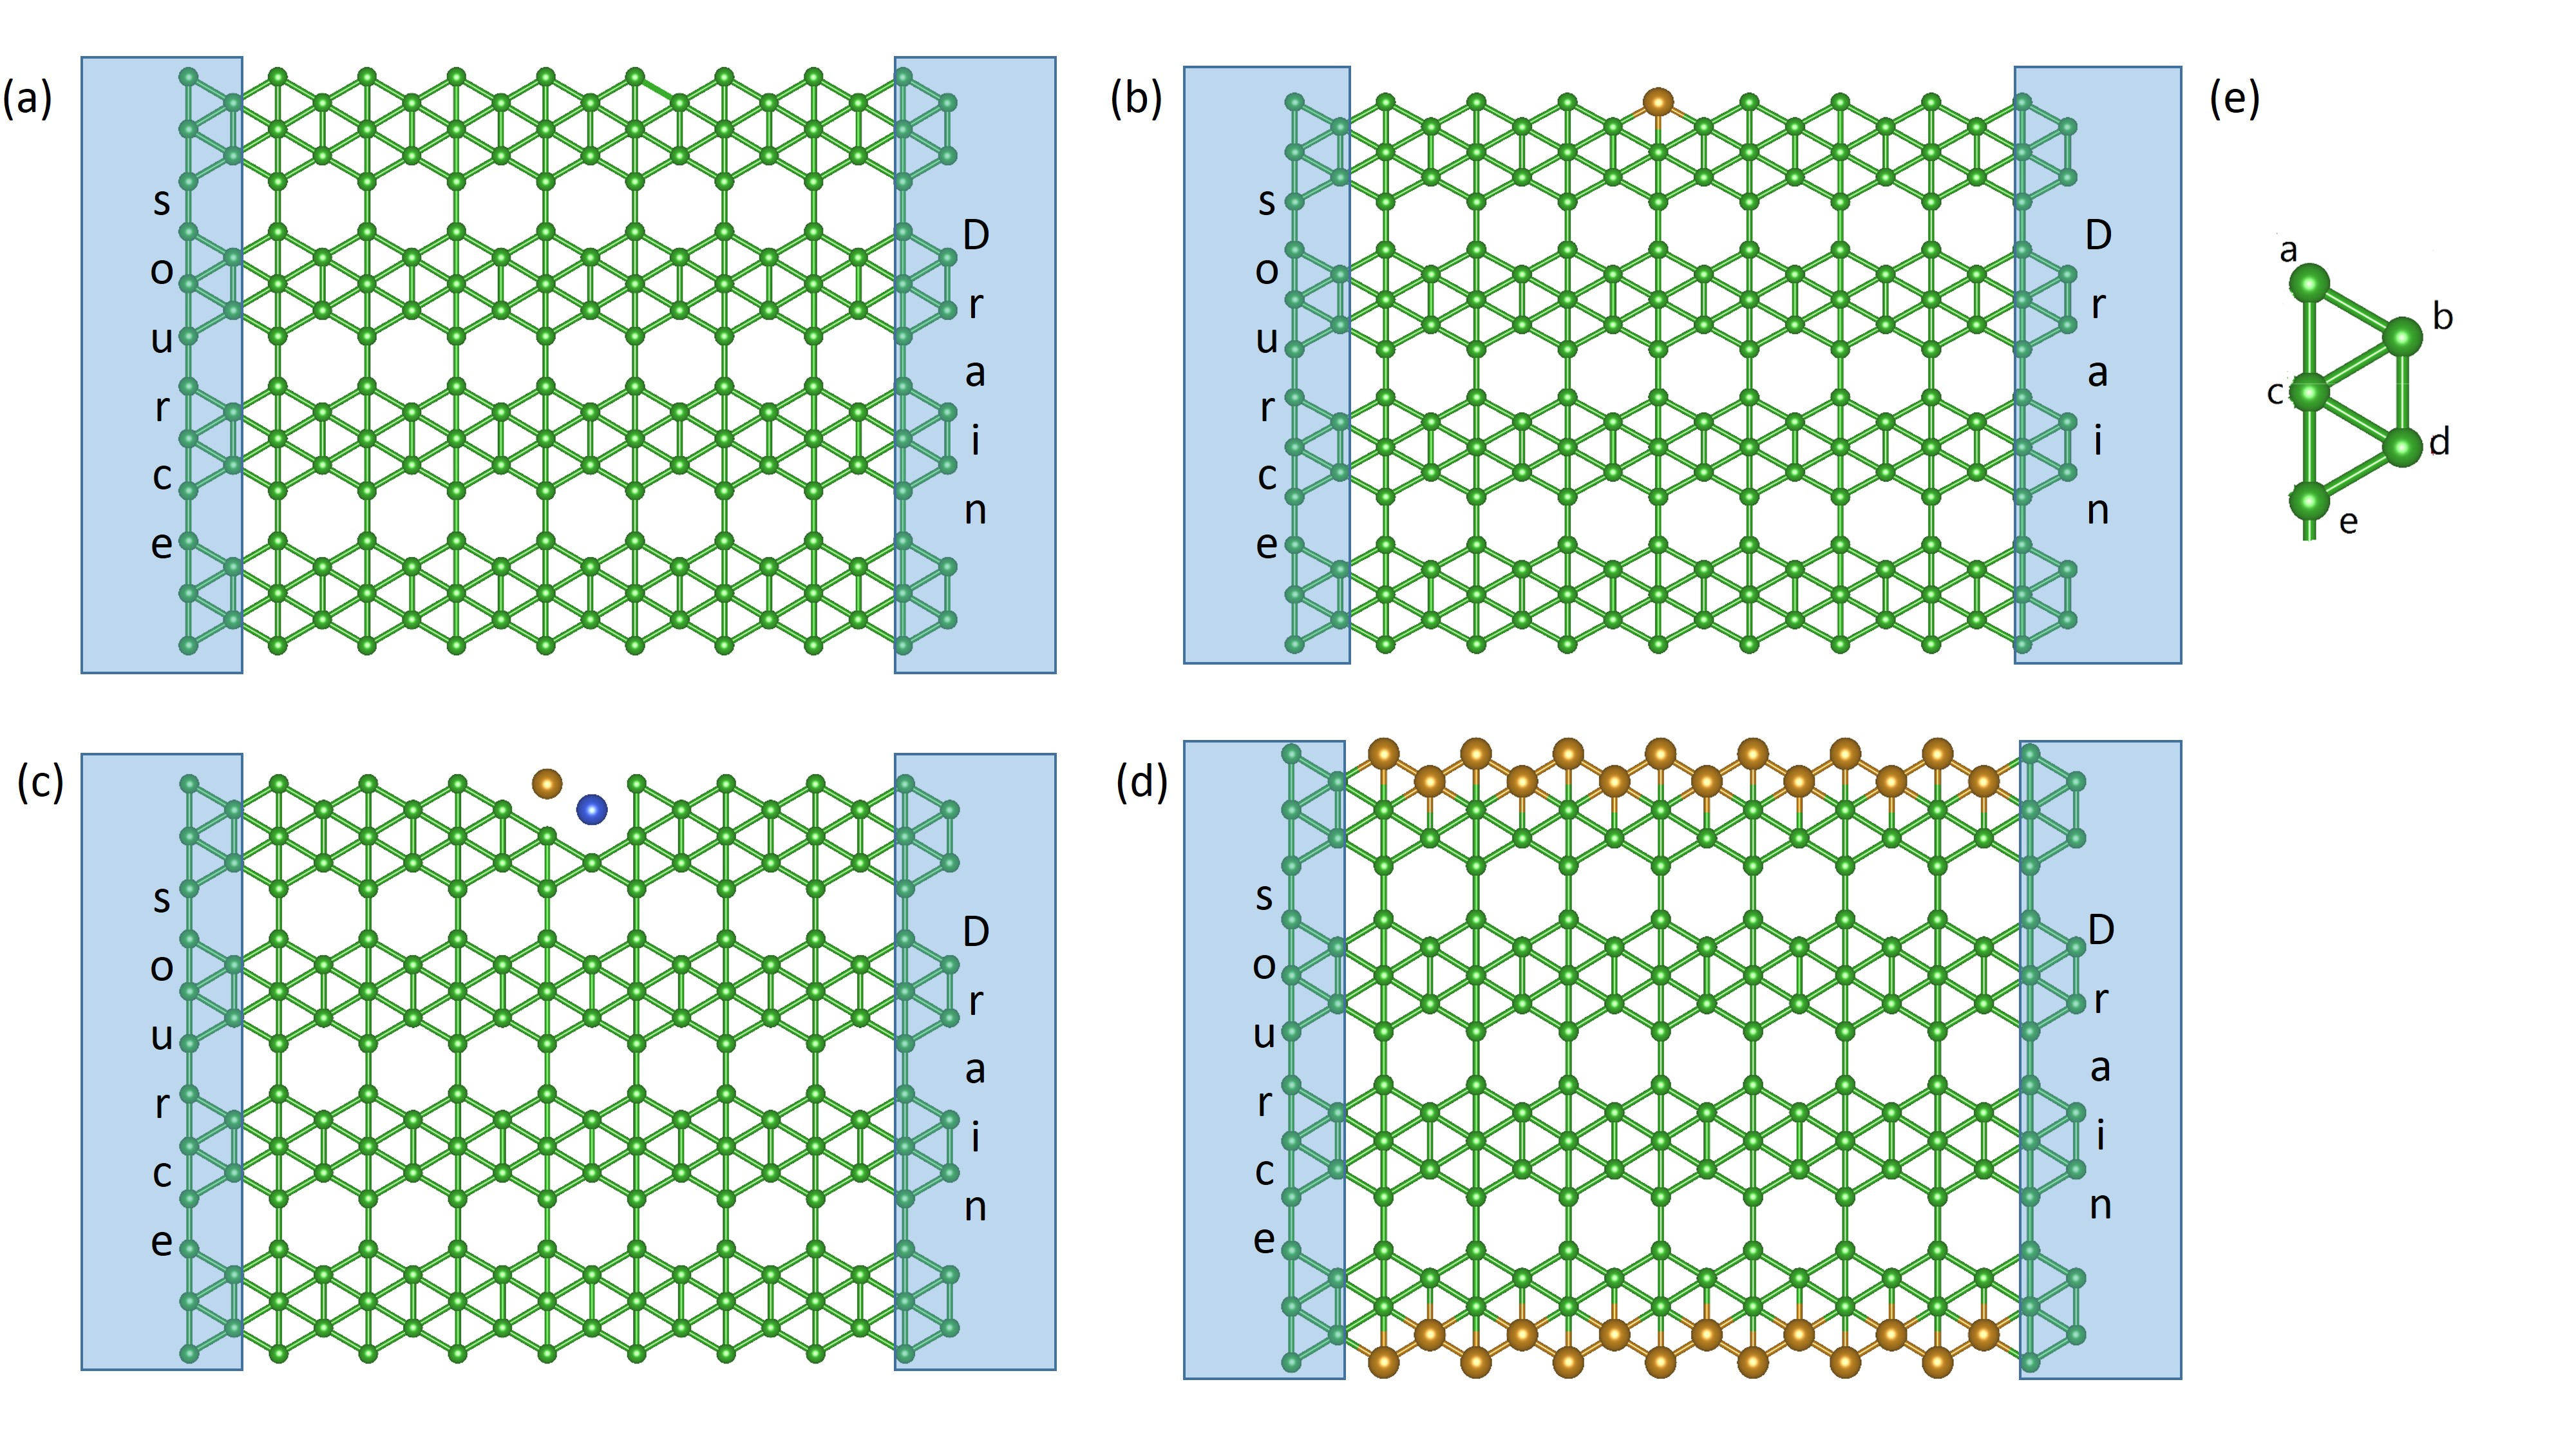
\includegraphics[width=1\linewidth]{./figures/borophene_structure(3).JPG}
    \caption{(الف) شماتیک نانوروبان زیگزاگ $\beta_{12}$-‌بورفین که این ساختار از یک شبکه مربعی با پایه تشکیل شده است.(ب) شماتیک یک نانوروبان زیگزاگ $\beta_{12}$-‌بورفین با ناخالصی لبه پراکنده.(ج) نمودار یک نانوروبان زیگزاگ $\beta_{12}$-‌بورفین با یک و دو جای خالی در لبه.(د) شماتیک نانوروبان زیگزاگ $\beta_{12}$-‌بورفین با اختلال لبه اندرسون.(ه) اساس شامل پنج اتم است که با \lr{a، b، c، d و e} نشان داده ‌‌می‌‌شوند.}
   \label{fig:borophene}
\end{figure*}
  \begin{figure}[!ht]
    \centering
    % GNUPLOT: LaTeX picture with Postscript
\begingroup
  % Encoding inside the plot.  In the header of your document, this encoding
  % should to defined, e.g., by using
  % \usepackage[cp1252,<other encodings>]{inputenc}
  % \inputencoding{cp1252}%
  \makeatletter
  \providecommand\color[2][]{%
    \GenericError{(gnuplot) \space\space\space\@spaces}{%
      Package color not loaded in conjunction with
      terminal option `colourtext'%
    }{See the gnuplot documentation for explanation.%
    }{Either use 'blacktext' in gnuplot or load the package
      color.sty in LaTeX.}%
    \renewcommand\color[2][]{}%
  }%
  \providecommand\includegraphics[2][]{%
    \GenericError{(gnuplot) \space\space\space\@spaces}{%
      Package graphicx or graphics not loaded%
    }{See the gnuplot documentation for explanation.%
    }{The gnuplot epslatex terminal needs graphicx.sty or graphics.sty.}%
    \renewcommand\includegraphics[2][]{}%
  }%
  \providecommand\rotatebox[2]{#2}%
  \@ifundefined{ifGPcolor}{%
    \newif\ifGPcolor
    \GPcolorfalse
  }{}%
  \@ifundefined{ifGPblacktext}{%
    \newif\ifGPblacktext
    \GPblacktexttrue
  }{}%
  % define a \g@addto@macro without @ in the name:
  \let\gplgaddtomacro\g@addto@macro
  % define empty templates for all commands taking text:
  \gdef\gplbacktext{}%
  \gdef\gplfronttext{}%
  \makeatother
  \ifGPblacktext
    % no textcolor at all
    \def\colorrgb#1{}%
    \def\colorgray#1{}%
  \else
    % gray or color?
    \ifGPcolor
      \def\colorrgb#1{\color[rgb]{#1}}%
      \def\colorgray#1{\color[gray]{#1}}%
      \expandafter\def\csname LTw\endcsname{\color{white}}%
      \expandafter\def\csname LTb\endcsname{\color{black}}%
      \expandafter\def\csname LTa\endcsname{\color{black}}%
      \expandafter\def\csname LT0\endcsname{\color[rgb]{1,0,0}}%
      \expandafter\def\csname LT1\endcsname{\color[rgb]{0,1,0}}%
      \expandafter\def\csname LT2\endcsname{\color[rgb]{0,0,1}}%
      \expandafter\def\csname LT3\endcsname{\color[rgb]{1,0,1}}%
      \expandafter\def\csname LT4\endcsname{\color[rgb]{0,1,1}}%
      \expandafter\def\csname LT5\endcsname{\color[rgb]{1,1,0}}%
      \expandafter\def\csname LT6\endcsname{\color[rgb]{0,0,0}}%
      \expandafter\def\csname LT7\endcsname{\color[rgb]{1,0.3,0}}%
      \expandafter\def\csname LT8\endcsname{\color[rgb]{0.5,0.5,0.5}}%
    \else
      % gray
      \def\colorrgb#1{\color{black}}%
      \def\colorgray#1{\color[gray]{#1}}%
      \expandafter\def\csname LTw\endcsname{\color{white}}%
      \expandafter\def\csname LTb\endcsname{\color{black}}%
      \expandafter\def\csname LTa\endcsname{\color{black}}%
      \expandafter\def\csname LT0\endcsname{\color{black}}%
      \expandafter\def\csname LT1\endcsname{\color{black}}%
      \expandafter\def\csname LT2\endcsname{\color{black}}%
      \expandafter\def\csname LT3\endcsname{\color{black}}%
      \expandafter\def\csname LT4\endcsname{\color{black}}%
      \expandafter\def\csname LT5\endcsname{\color{black}}%
      \expandafter\def\csname LT6\endcsname{\color{black}}%
      \expandafter\def\csname LT7\endcsname{\color{black}}%
      \expandafter\def\csname LT8\endcsname{\color{black}}%
    \fi
  \fi
    \setlength{\unitlength}{0.0500bp}%
    \ifx\gptboxheight\undefined%
      \newlength{\gptboxheight}%
      \newlength{\gptboxwidth}%
      \newsavebox{\gptboxtext}%
    \fi%
    \setlength{\fboxrule}{0.5pt}%
    \setlength{\fboxsep}{1pt}%
\begin{picture}(4320.00,5760.00)%
    \gplgaddtomacro\gplbacktext{%
      \csname LTb\endcsname%%
      \put(300,3320){\makebox(0,0)[r]{\strut{}$0$}}%
      \put(300,3567){\makebox(0,0)[r]{\strut{}$1$}}%
      \put(300,3813){\makebox(0,0)[r]{\strut{}$2$}}%
      \put(300,4060){\makebox(0,0)[r]{\strut{}$3$}}%
      \put(300,4306){\makebox(0,0)[r]{\strut{}$4$}}%
      \put(300,4553){\makebox(0,0)[r]{\strut{}$5$}}%
      \put(300,4799){\makebox(0,0)[r]{\strut{}$6$}}%
      \put(300,5046){\makebox(0,0)[r]{\strut{}$7$}}%
      \put(300,5292){\makebox(0,0)[r]{\strut{}$8$}}%
      \put(300,5539){\makebox(0,0)[r]{\strut{}$9$}}%
      \put(432,3100){\makebox(0,0){\strut{}$-2$}}%
      \put(866,3100){\makebox(0,0){\strut{}$-1.5$}}%
      \put(1300,3100){\makebox(0,0){\strut{}$-1$}}%
      \put(1735,3100){\makebox(0,0){\strut{}$-0.5$}}%
      \put(2169,3100){\makebox(0,0){\strut{}$0$}}%
      \put(2603,3100){\makebox(0,0){\strut{}$0.5$}}%
      \put(3037,3100){\makebox(0,0){\strut{}$1$}}%
      \put(3471,3100){\makebox(0,0){\strut{}$1.5$}}%
      \put(3906,3100){\makebox(0,0){\strut{}$2$}}%
      \put(607,5428){\makebox(0,0)[l]{\strut{}(a)}}%
    }%
    \gplgaddtomacro\gplfronttext{%
      \csname LTb\endcsname%%
      \put(-52,4429){\rotatebox{-270}{\makebox(0,0){\strut{}$G/G_0$}}}%
      \csname LTb\endcsname%%
      \put(2936,5366){\makebox(0,0)[r]{\strut{}Pristine-$\beta_{12}$}}%
      \csname LTb\endcsname%%
      \put(2936,5146){\makebox(0,0)[r]{\strut{}V=1 eV}}%
      \csname LTb\endcsname%%
      \put(2936,4926){\makebox(0,0)[r]{\strut{}V=2 eV}}%
      \csname LTb\endcsname%%
      \put(2936,4706){\makebox(0,0)[r]{\strut{}V=5 eV}}%
    }%
    \gplgaddtomacro\gplbacktext{%
      \csname LTb\endcsname%%
      \put(300,704){\makebox(0,0)[r]{\strut{}$0$}}%
      \put(300,1193){\makebox(0,0)[r]{\strut{}$0.05$}}%
      \put(300,1682){\makebox(0,0)[r]{\strut{}$0.1$}}%
      \put(300,2171){\makebox(0,0)[r]{\strut{}$0.15$}}%
      \put(300,2660){\makebox(0,0)[r]{\strut{}$0.2$}}%
      \put(432,484){\makebox(0,0){\strut{}$-2$}}%
      \put(866,484){\makebox(0,0){\strut{}$-1.5$}}%
      \put(1300,484){\makebox(0,0){\strut{}$-1$}}%
      \put(1735,484){\makebox(0,0){\strut{}$-0.5$}}%
      \put(2169,484){\makebox(0,0){\strut{}$0$}}%
      \put(2603,484){\makebox(0,0){\strut{}$0.5$}}%
      \put(3037,484){\makebox(0,0){\strut{}$1$}}%
      \put(3471,484){\makebox(0,0){\strut{}$1.5$}}%
      \put(3906,484){\makebox(0,0){\strut{}$2$}}%
      \put(607,2562){\makebox(0,0)[l]{\strut{}(b)}}%
    }%
    \gplgaddtomacro\gplfronttext{%
      \csname LTb\endcsname%%
      \put(-448,1682){\rotatebox{-270}{\makebox(0,0){\strut{}LDOS}}}%
      \put(2177,154){\makebox(0,0){\strut{}Energy(eV)}}%
    }%
    \gplbacktext
    \put(0,0){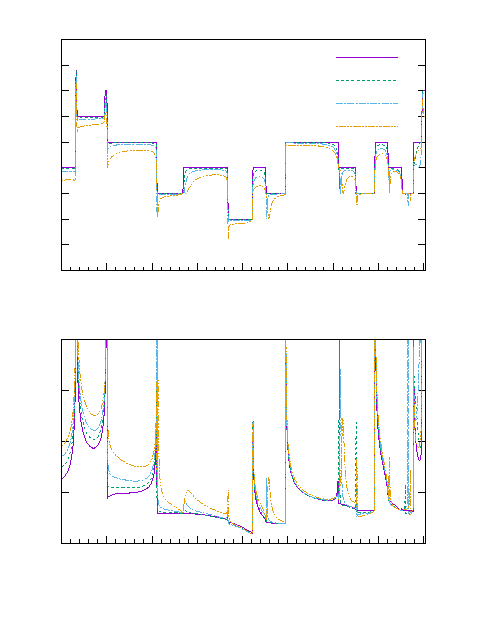
\includegraphics[width={217.00bp},height={289.00bp}]{zigscatter}}%
    \gplfronttext
  \end{picture}%
\endgroup

    \caption{الف) رسانایی نانو نوارهای زیگزاگی با عرض \lr{\AA}18.59 و طول \lr{\AA} 42.34، با ناخالصی واقع در لبه بالایی یک سوپرسل در نانو نوار. (ب) چگالی الکترونی حالات در نزدیکترین محل همسایه ناخالصی که همان الف.}
    \label{zigscatter}
  \end{figure}
  \begin{figure}[ht]
    \centering
    % GNUPLOT: LaTeX picture with Postscript
\begingroup
  % Encoding inside the plot.  In the header of your document, this encoding
  % should to defined, e.g., by using
  % \usepackage[cp1252,<other encodings>]{inputenc}
  % \inputencoding{cp1252}%
  \makeatletter
  \providecommand\color[2][]{%
    \GenericError{(gnuplot) \space\space\space\@spaces}{%
      Package color not loaded in conjunction with
      terminal option `colourtext'%
    }{See the gnuplot documentation for explanation.%
    }{Either use 'blacktext' in gnuplot or load the package
      color.sty in LaTeX.}%
    \renewcommand\color[2][]{}%
  }%
  \providecommand\includegraphics[2][]{%
    \GenericError{(gnuplot) \space\space\space\@spaces}{%
      Package graphicx or graphics not loaded%
    }{See the gnuplot documentation for explanation.%
    }{The gnuplot epslatex terminal needs graphicx.sty or graphics.sty.}%
    \renewcommand\includegraphics[2][]{}%
  }%
  \providecommand\rotatebox[2]{#2}%
  \@ifundefined{ifGPcolor}{%
    \newif\ifGPcolor
    \GPcolorfalse
  }{}%
  \@ifundefined{ifGPblacktext}{%
    \newif\ifGPblacktext
    \GPblacktexttrue
  }{}%
  % define a \g@addto@macro without @ in the name:
  \let\gplgaddtomacro\g@addto@macro
  % define empty templates for all commands taking text:
  \gdef\gplbacktext{}%
  \gdef\gplfronttext{}%
  \makeatother
  \ifGPblacktext
    % no textcolor at all
    \def\colorrgb#1{}%
    \def\colorgray#1{}%
  \else
    % gray or color?
    \ifGPcolor
      \def\colorrgb#1{\color[rgb]{#1}}%
      \def\colorgray#1{\color[gray]{#1}}%
      \expandafter\def\csname LTw\endcsname{\color{white}}%
      \expandafter\def\csname LTb\endcsname{\color{black}}%
      \expandafter\def\csname LTa\endcsname{\color{black}}%
      \expandafter\def\csname LT0\endcsname{\color[rgb]{1,0,0}}%
      \expandafter\def\csname LT1\endcsname{\color[rgb]{0,1,0}}%
      \expandafter\def\csname LT2\endcsname{\color[rgb]{0,0,1}}%
      \expandafter\def\csname LT3\endcsname{\color[rgb]{1,0,1}}%
      \expandafter\def\csname LT4\endcsname{\color[rgb]{0,1,1}}%
      \expandafter\def\csname LT5\endcsname{\color[rgb]{1,1,0}}%
      \expandafter\def\csname LT6\endcsname{\color[rgb]{0,0,0}}%
      \expandafter\def\csname LT7\endcsname{\color[rgb]{1,0.3,0}}%
      \expandafter\def\csname LT8\endcsname{\color[rgb]{0.5,0.5,0.5}}%
    \else
      % gray
      \def\colorrgb#1{\color{black}}%
      \def\colorgray#1{\color[gray]{#1}}%
      \expandafter\def\csname LTw\endcsname{\color{white}}%
      \expandafter\def\csname LTb\endcsname{\color{black}}%
      \expandafter\def\csname LTa\endcsname{\color{black}}%
      \expandafter\def\csname LT0\endcsname{\color{black}}%
      \expandafter\def\csname LT1\endcsname{\color{black}}%
      \expandafter\def\csname LT2\endcsname{\color{black}}%
      \expandafter\def\csname LT3\endcsname{\color{black}}%
      \expandafter\def\csname LT4\endcsname{\color{black}}%
      \expandafter\def\csname LT5\endcsname{\color{black}}%
      \expandafter\def\csname LT6\endcsname{\color{black}}%
      \expandafter\def\csname LT7\endcsname{\color{black}}%
      \expandafter\def\csname LT8\endcsname{\color{black}}%
    \fi
  \fi
    \setlength{\unitlength}{0.0500bp}%
    \ifx\gptboxheight\undefined%
      \newlength{\gptboxheight}%
      \newlength{\gptboxwidth}%
      \newsavebox{\gptboxtext}%
    \fi%
    \setlength{\fboxrule}{0.5pt}%
    \setlength{\fboxsep}{1pt}%
\begin{picture}(4320.00,5760.00)%
    \gplgaddtomacro\gplbacktext{%
      \csname LTb\endcsname%%
      \put(300,3320){\makebox(0,0)[r]{\strut{}$0$}}%
      \put(300,3597){\makebox(0,0)[r]{\strut{}$1$}}%
      \put(300,3875){\makebox(0,0)[r]{\strut{}$2$}}%
      \put(300,4152){\makebox(0,0)[r]{\strut{}$3$}}%
      \put(300,4430){\makebox(0,0)[r]{\strut{}$4$}}%
      \put(300,4707){\makebox(0,0)[r]{\strut{}$5$}}%
      \put(300,4984){\makebox(0,0)[r]{\strut{}$6$}}%
      \put(300,5262){\makebox(0,0)[r]{\strut{}$7$}}%
      \put(300,5539){\makebox(0,0)[r]{\strut{}$8$}}%
      \put(432,3100){\makebox(0,0){\strut{}$-2$}}%
      \put(868,3100){\makebox(0,0){\strut{}$-1.5$}}%
      \put(1305,3100){\makebox(0,0){\strut{}$-1$}}%
      \put(1741,3100){\makebox(0,0){\strut{}$-0.5$}}%
      \put(2178,3100){\makebox(0,0){\strut{}$0$}}%
      \put(2614,3100){\makebox(0,0){\strut{}$0.5$}}%
      \put(3050,3100){\makebox(0,0){\strut{}$1$}}%
      \put(3487,3100){\makebox(0,0){\strut{}$1.5$}}%
      \put(3923,3100){\makebox(0,0){\strut{}$2$}}%
      \put(676,5428){\makebox(0,0)[l]{\strut{}(a)}}%
    }%
    \gplgaddtomacro\gplfronttext{%
      \csname LTb\endcsname%%
      \put(-52,4429){\rotatebox{-270}{\makebox(0,0){\strut{}$G/G_0$}}}%
      \csname LTb\endcsname%%
      \put(2936,5366){\makebox(0,0)[r]{\strut{}Pristine-$\beta_{12}$}}%
      \csname LTb\endcsname%%
      \put(2936,5146){\makebox(0,0)[r]{\strut{}V=1 eV}}%
      \csname LTb\endcsname%%
      \put(2936,4926){\makebox(0,0)[r]{\strut{}V=2 eV}}%
      \csname LTb\endcsname%%
      \put(2936,4706){\makebox(0,0)[r]{\strut{}V=5 eV}}%
    }%
    \gplgaddtomacro\gplbacktext{%
      \csname LTb\endcsname%%
      \put(300,704){\makebox(0,0)[r]{\strut{}$0$}}%
      \put(300,1095){\makebox(0,0)[r]{\strut{}$0.1$}}%
      \put(300,1486){\makebox(0,0)[r]{\strut{}$0.2$}}%
      \put(300,1878){\makebox(0,0)[r]{\strut{}$0.3$}}%
      \put(300,2269){\makebox(0,0)[r]{\strut{}$0.4$}}%
      \put(300,2660){\makebox(0,0)[r]{\strut{}$0.5$}}%
      \put(432,484){\makebox(0,0){\strut{}$-2$}}%
      \put(868,484){\makebox(0,0){\strut{}$-1.5$}}%
      \put(1305,484){\makebox(0,0){\strut{}$-1$}}%
      \put(1741,484){\makebox(0,0){\strut{}$-0.5$}}%
      \put(2178,484){\makebox(0,0){\strut{}$0$}}%
      \put(2614,484){\makebox(0,0){\strut{}$0.5$}}%
      \put(3050,484){\makebox(0,0){\strut{}$1$}}%
      \put(3487,484){\makebox(0,0){\strut{}$1.5$}}%
      \put(3923,484){\makebox(0,0){\strut{}$2$}}%
      \put(676,2562){\makebox(0,0)[l]{\strut{}(b)}}%
    }%
    \gplgaddtomacro\gplfronttext{%
      \csname LTb\endcsname%%
      \put(-316,1682){\rotatebox{-270}{\makebox(0,0){\strut{}LDOS}}}%
      \put(2177,154){\makebox(0,0){\strut{}Energy(eV)}}%
    }%
    \gplbacktext
    \put(0,0){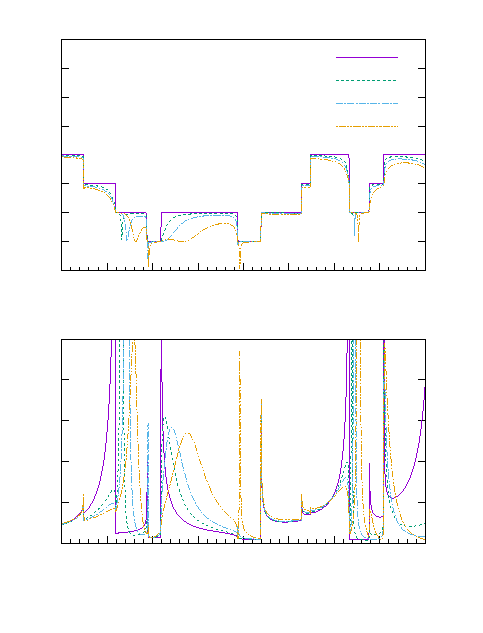
\includegraphics[width={217.00bp},height={289.00bp}]{armscatter}}%
    \gplfronttext
  \end{picture}%
\endgroup

    \caption{(الف) رسانایی نانو نوارهای آرمچیر آرمچیر با عرض \lr{\AA} 10.24 و طول \lr{\AA} 74.36 با ناخالصی واقع در لبه بالایی یک سوپرسل در نانو نوار. (ب) چگالی الکترونی حالات در نزدیکترین محل همسایه ناخالصی که همان a.}
    \label{armscatter}
  \end{figure}

\begin{figure}[ht]
    \centering
    % GNUPLOT: LaTeX picture with Postscript
\begingroup
  % Encoding inside the plot.  In the header of your document, this encoding
  % should to defined, e.g., by using
  % \usepackage[cp1252,<other encodings>]{inputenc}
  % \inputencoding{cp1252}%
  \makeatletter
  \providecommand\color[2][]{%
    \GenericError{(gnuplot) \space\space\space\@spaces}{%
      Package color not loaded in conjunction with
      terminal option `colourtext'%
    }{See the gnuplot documentation for explanation.%
    }{Either use 'blacktext' in gnuplot or load the package
      color.sty in LaTeX.}%
    \renewcommand\color[2][]{}%
  }%
  \providecommand\includegraphics[2][]{%
    \GenericError{(gnuplot) \space\space\space\@spaces}{%
      Package graphicx or graphics not loaded%
    }{See the gnuplot documentation for explanation.%
    }{The gnuplot epslatex terminal needs graphicx.sty or graphics.sty.}%
    \renewcommand\includegraphics[2][]{}%
  }%
  \providecommand\rotatebox[2]{#2}%
  \@ifundefined{ifGPcolor}{%
    \newif\ifGPcolor
    \GPcolorfalse
  }{}%
  \@ifundefined{ifGPblacktext}{%
    \newif\ifGPblacktext
    \GPblacktexttrue
  }{}%
  % define a \g@addto@macro without @ in the name:
  \let\gplgaddtomacro\g@addto@macro
  % define empty templates for all commands taking text:
  \gdef\gplbacktext{}%
  \gdef\gplfronttext{}%
  \makeatother
  \ifGPblacktext
    % no textcolor at all
    \def\colorrgb#1{}%
    \def\colorgray#1{}%
  \else
    % gray or color?
    \ifGPcolor
      \def\colorrgb#1{\color[rgb]{#1}}%
      \def\colorgray#1{\color[gray]{#1}}%
      \expandafter\def\csname LTw\endcsname{\color{white}}%
      \expandafter\def\csname LTb\endcsname{\color{black}}%
      \expandafter\def\csname LTa\endcsname{\color{black}}%
      \expandafter\def\csname LT0\endcsname{\color[rgb]{1,0,0}}%
      \expandafter\def\csname LT1\endcsname{\color[rgb]{0,1,0}}%
      \expandafter\def\csname LT2\endcsname{\color[rgb]{0,0,1}}%
      \expandafter\def\csname LT3\endcsname{\color[rgb]{1,0,1}}%
      \expandafter\def\csname LT4\endcsname{\color[rgb]{0,1,1}}%
      \expandafter\def\csname LT5\endcsname{\color[rgb]{1,1,0}}%
      \expandafter\def\csname LT6\endcsname{\color[rgb]{0,0,0}}%
      \expandafter\def\csname LT7\endcsname{\color[rgb]{1,0.3,0}}%
      \expandafter\def\csname LT8\endcsname{\color[rgb]{0.5,0.5,0.5}}%
    \else
      % gray
      \def\colorrgb#1{\color{black}}%
      \def\colorgray#1{\color[gray]{#1}}%
      \expandafter\def\csname LTw\endcsname{\color{white}}%
      \expandafter\def\csname LTb\endcsname{\color{black}}%
      \expandafter\def\csname LTa\endcsname{\color{black}}%
      \expandafter\def\csname LT0\endcsname{\color{black}}%
      \expandafter\def\csname LT1\endcsname{\color{black}}%
      \expandafter\def\csname LT2\endcsname{\color{black}}%
      \expandafter\def\csname LT3\endcsname{\color{black}}%
      \expandafter\def\csname LT4\endcsname{\color{black}}%
      \expandafter\def\csname LT5\endcsname{\color{black}}%
      \expandafter\def\csname LT6\endcsname{\color{black}}%
      \expandafter\def\csname LT7\endcsname{\color{black}}%
      \expandafter\def\csname LT8\endcsname{\color{black}}%
    \fi
  \fi
    \setlength{\unitlength}{0.0500bp}%
    \ifx\gptboxheight\undefined%
      \newlength{\gptboxheight}%
      \newlength{\gptboxwidth}%
      \newsavebox{\gptboxtext}%
    \fi%
    \setlength{\fboxrule}{0.5pt}%
    \setlength{\fboxsep}{1pt}%
\begin{picture}(4320.00,5760.00)%
    \gplgaddtomacro\gplbacktext{%
      \csname LTb\endcsname%%
      \put(300,3320){\makebox(0,0)[r]{\strut{}$0$}}%
      \put(300,3597){\makebox(0,0)[r]{\strut{}$1$}}%
      \put(300,3875){\makebox(0,0)[r]{\strut{}$2$}}%
      \put(300,4152){\makebox(0,0)[r]{\strut{}$3$}}%
      \put(300,4430){\makebox(0,0)[r]{\strut{}$4$}}%
      \put(300,4707){\makebox(0,0)[r]{\strut{}$5$}}%
      \put(300,4984){\makebox(0,0)[r]{\strut{}$6$}}%
      \put(300,5262){\makebox(0,0)[r]{\strut{}$7$}}%
      \put(300,5539){\makebox(0,0)[r]{\strut{}$8$}}%
      \put(432,3100){\makebox(0,0){\strut{}$-2$}}%
      \put(866,3100){\makebox(0,0){\strut{}$-1.5$}}%
      \put(1300,3100){\makebox(0,0){\strut{}$-1$}}%
      \put(1735,3100){\makebox(0,0){\strut{}$-0.5$}}%
      \put(2169,3100){\makebox(0,0){\strut{}$0$}}%
      \put(2603,3100){\makebox(0,0){\strut{}$0.5$}}%
      \put(3037,3100){\makebox(0,0){\strut{}$1$}}%
      \put(3471,3100){\makebox(0,0){\strut{}$1.5$}}%
      \put(3906,3100){\makebox(0,0){\strut{}$2$}}%
      \put(676,5428){\makebox(0,0)[l]{\strut{}(a)}}%
    }%
    \gplgaddtomacro\gplfronttext{%
      \csname LTb\endcsname%%
      \put(-52,4429){\rotatebox{-270}{\makebox(0,0){\strut{}$G/G_0$}}}%
      \csname LTb\endcsname%%
      \put(2936,5366){\makebox(0,0)[r]{\strut{}Pristine-$\beta_{12}$}}%
      \csname LTb\endcsname%%
      \put(2936,5146){\makebox(0,0)[r]{\strut{}One edge Vacancy}}%
      \csname LTb\endcsname%%
      \put(2936,4926){\makebox(0,0)[r]{\strut{}Two edges Vacancies}}%
    }%
    \gplgaddtomacro\gplbacktext{%
      \csname LTb\endcsname%%
      \put(300,704){\makebox(0,0)[r]{\strut{}$0$}}%
      \put(300,1095){\makebox(0,0)[r]{\strut{}$0.1$}}%
      \put(300,1486){\makebox(0,0)[r]{\strut{}$0.2$}}%
      \put(300,1878){\makebox(0,0)[r]{\strut{}$0.3$}}%
      \put(300,2269){\makebox(0,0)[r]{\strut{}$0.4$}}%
      \put(300,2660){\makebox(0,0)[r]{\strut{}$0.5$}}%
      \put(432,484){\makebox(0,0){\strut{}$-2$}}%
      \put(868,484){\makebox(0,0){\strut{}$-1.5$}}%
      \put(1305,484){\makebox(0,0){\strut{}$-1$}}%
      \put(1741,484){\makebox(0,0){\strut{}$-0.5$}}%
      \put(2178,484){\makebox(0,0){\strut{}$0$}}%
      \put(2614,484){\makebox(0,0){\strut{}$0.5$}}%
      \put(3050,484){\makebox(0,0){\strut{}$1$}}%
      \put(3487,484){\makebox(0,0){\strut{}$1.5$}}%
      \put(3923,484){\makebox(0,0){\strut{}$2$}}%
      \put(676,2562){\makebox(0,0)[l]{\strut{}(b)}}%
    }%
    \gplgaddtomacro\gplfronttext{%
      \csname LTb\endcsname%%
      \put(-316,1682){\rotatebox{-270}{\makebox(0,0){\strut{}LDOS}}}%
      \put(2177,154){\makebox(0,0){\strut{}Energy(eV)}}%
    }%
    \gplbacktext
    \put(0,0){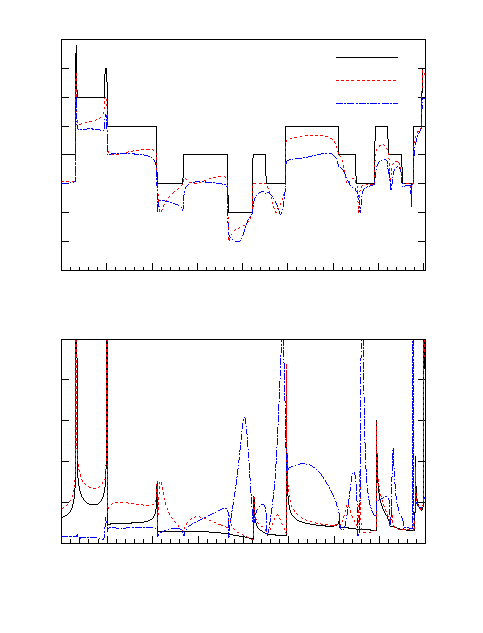
\includegraphics[width={217.00bp},height={289.00bp}]{zigvacancy}}%
    \gplfronttext
  \end{picture}%
\endgroup

    \caption{(الف) رسانایی نانو نوارهای زیگزاگی با
    عرض \lr{\AA} 18.59 و طول \lr{\AA} 42.34، با جاهای خالی در لبه بالایی سوپرسل ‌میانی قرار دارد.(ب) چگالی الکترونی حالات در نزدیکترین محل همسایه جاهای خالی واقع در همان (الف).}
    \label{zigvacancy}
  \end{figure}
  
\begin{figure}[ht]
\centering
% GNUPLOT: LaTeX picture with Postscript
\begin{latin}
\begingroup
  \makeatletter
  \providecommand\color[2][]{%
    \GenericError{(gnuplot) \space\space\space\@spaces}{%
      Package color not loaded in conjunction with
      terminal option `colourtext'%
    }{See the gnuplot documentation for explanation.%
    }{Either use 'blacktext' in gnuplot or load the package
      color.sty in LaTeX.}%
    \renewcommand\color[2][]{}%
  }%
  \providecommand\includegraphics[2][]{%
    \GenericError{(gnuplot) \space\space\space\@spaces}{%
      Package graphicx or graphics not loaded%
    }{See the gnuplot documentation for explanation.%
    }{The gnuplot epslatex terminal needs graphicx.sty or graphics.sty.}%
    \renewcommand\includegraphics[2][]{}%
  }%
  \providecommand\rotatebox[2]{#2}%
  \@ifundefined{ifGPcolor}{%
    \newif\ifGPcolor
    \GPcolorfalse
  }{}%
  \@ifundefined{ifGPblacktext}{%
    \newif\ifGPblacktext
    \GPblacktexttrue
  }{}%
  % define a \g@addto@macro without @ in the name:
  \let\gplgaddtomacro\g@addto@macro
  % define empty templates for all commands taking text:
  \gdef\gplbacktext{}%
  \gdef\gplfronttext{}%
  \makeatother
  \ifGPblacktext
    % no textcolor at all
    \def\colorrgb#1{}%
    \def\colorgray#1{}%
  \else
    % gray or color?
    \ifGPcolor
      \def\colorrgb#1{\color[rgb]{#1}}%
      \def\colorgray#1{\color[gray]{#1}}%
      \expandafter\def\csname LTw\endcsname{\color{white}}%
      \expandafter\def\csname LTb\endcsname{\color{black}}%
      \expandafter\def\csname LTa\endcsname{\color{black}}%
      \expandafter\def\csname LT0\endcsname{\color[rgb]{1,0,0}}%
      \expandafter\def\csname LT1\endcsname{\color[rgb]{0,1,0}}%
      \expandafter\def\csname LT2\endcsname{\color[rgb]{0,0,1}}%
      \expandafter\def\csname LT3\endcsname{\color[rgb]{1,0,1}}%
      \expandafter\def\csname LT4\endcsname{\color[rgb]{0,1,1}}%
      \expandafter\def\csname LT5\endcsname{\color[rgb]{1,1,0}}%
      \expandafter\def\csname LT6\endcsname{\color[rgb]{0,0,0}}%
      \expandafter\def\csname LT7\endcsname{\color[rgb]{1,0.3,0}}%
      \expandafter\def\csname LT8\endcsname{\color[rgb]{0.5,0.5,0.5}}%
    \else
      % gray
      \def\colorrgb#1{\color{black}}%
      \def\colorgray#1{\color[gray]{#1}}%
      \expandafter\def\csname LTw\endcsname{\color{white}}%
      \expandafter\def\csname LTb\endcsname{\color{black}}%
      \expandafter\def\csname LTa\endcsname{\color{black}}%
      \expandafter\def\csname LT0\endcsname{\color{black}}%
      \expandafter\def\csname LT1\endcsname{\color{black}}%
      \expandafter\def\csname LT2\endcsname{\color{black}}%
      \expandafter\def\csname LT3\endcsname{\color{black}}%
      \expandafter\def\csname LT4\endcsname{\color{black}}%
      \expandafter\def\csname LT5\endcsname{\color{black}}%
      \expandafter\def\csname LT6\endcsname{\color{black}}%
      \expandafter\def\csname LT7\endcsname{\color{black}}%
      \expandafter\def\csname LT8\endcsname{\color{black}}%
    \fi
  \fi
    \setlength{\unitlength}{0.0500bp}%
    \ifx\gptboxheight\undefined%
      \newlength{\gptboxheight}%
      \newlength{\gptboxwidth}%
      \newsavebox{\gptboxtext}%
    \fi%
    \setlength{\fboxrule}{0.5pt}%
    \setlength{\fboxsep}{1pt}%
\begin{picture}(4320.00,5760.00)%
    \gplgaddtomacro\gplbacktext{%
      \csname LTb\endcsname%%
      \put(300,3320){\makebox(0,0)[r]{\strut{}$0$}}%
      \put(300,3597){\makebox(0,0)[r]{\strut{}$1$}}%
      \put(300,3875){\makebox(0,0)[r]{\strut{}$2$}}%
      \put(300,4152){\makebox(0,0)[r]{\strut{}$3$}}%
      \put(300,4430){\makebox(0,0)[r]{\strut{}$4$}}%
      \put(300,4707){\makebox(0,0)[r]{\strut{}$5$}}%
      \put(300,4984){\makebox(0,0)[r]{\strut{}$6$}}%
      \put(300,5262){\makebox(0,0)[r]{\strut{}$7$}}%
      \put(300,5539){\makebox(0,0)[r]{\strut{}$8$}}%
      \put(432,3100){\makebox(0,0){\strut{}$-2$}}%
      \put(868,3100){\makebox(0,0){\strut{}$-1.5$}}%
      \put(1305,3100){\makebox(0,0){\strut{}$-1$}}%
      \put(1741,3100){\makebox(0,0){\strut{}$-0.5$}}%
      \put(2178,3100){\makebox(0,0){\strut{}$0$}}%
      \put(2614,3100){\makebox(0,0){\strut{}$0.5$}}%
      \put(3050,3100){\makebox(0,0){\strut{}$1$}}%
      \put(3487,3100){\makebox(0,0){\strut{}$1.5$}}%
      \put(3923,3100){\makebox(0,0){\strut{}$2$}}%
      \put(711,5428){\makebox(0,0)[l]{\strut{}(a)}}%
    }%
    \gplgaddtomacro\gplfronttext{%
      \csname LTb\endcsname%%
      \put(-52,4429){\rotatebox{-270}{\makebox(0,0){\strut{}$G/G_0$}}}%
      \csname LTb\endcsname%%
      \put(2936,5366){\makebox(0,0)[r]{\strut{}Pristine-$\beta_{12}$}}%
      \csname LTb\endcsname%%
      \put(2936,5146){\makebox(0,0)[r]{\strut{}One edge Vacancy}}%
      \csname LTb\endcsname%%
      \put(2936,4926){\makebox(0,0)[r]{\strut{}Two edges Vacancies}}%
    }%
    \gplgaddtomacro\gplbacktext{%
      \csname LTb\endcsname%%
      \put(300,704){\makebox(0,0)[r]{\strut{}$0$}}%
      \put(300,1095){\makebox(0,0)[r]{\strut{}$0.2$}}%
      \put(300,1486){\makebox(0,0)[r]{\strut{}$0.4$}}%
      \put(300,1878){\makebox(0,0)[r]{\strut{}$0.6$}}%
      \put(300,2269){\makebox(0,0)[r]{\strut{}$0.8$}}%
      \put(300,2660){\makebox(0,0)[r]{\strut{}$1$}}%
      \put(432,484){\makebox(0,0){\strut{}$-2$}}%
      \put(868,484){\makebox(0,0){\strut{}$-1.5$}}%
      \put(1305,484){\makebox(0,0){\strut{}$-1$}}%
      \put(1741,484){\makebox(0,0){\strut{}$-0.5$}}%
      \put(2178,484){\makebox(0,0){\strut{}$0$}}%
      \put(2614,484){\makebox(0,0){\strut{}$0.5$}}%
      \put(3050,484){\makebox(0,0){\strut{}$1$}}%
      \put(3487,484){\makebox(0,0){\strut{}$1.5$}}%
      \put(3923,484){\makebox(0,0){\strut{}$2$}}%
      \put(711,2562){\makebox(0,0)[l]{\strut{}(b)}}%
    }%
    \gplgaddtomacro\gplfronttext{%
      \csname LTb\endcsname%%
      \put(-316,1682){\rotatebox{-270}{\makebox(0,0){\strut{}LDOS}}}%
      \put(2177,154){\makebox(0,0){\strut{}Energy(eV)}}%
    }%
    \gplbacktext
    \put(0,0){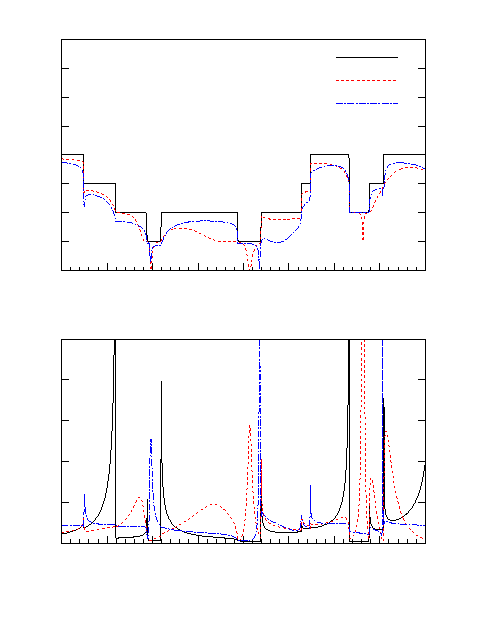
\includegraphics[width={217.00bp},height={289.00bp}]{armvacancy}}%
    \gplfronttext
  \end{picture}%
\endgroup
\end{latin}
\caption{(الف) رسانایی نانو نوارهای آرمچیر آرمچیر با
عرض \lr{\AA} 10.24 و طول \lr{\AA} 74.36، با جاهای خالی واقع در لبه بالایی سوپرسل ‌میانی از نانوروبان. (ب) چگالی الکترونی حالات در نزدیکترین محل همسایه جاهای خالی واقع مشابه (الف).}
\label{armvacancy}
\end{figure}
\subsection{عیوب منفرد:} 
به منظور توصیف اثر عیوب لبه بر الکترونیک و ترابرد نانو نوارهای شبکه لانه زنبوری، اجازه دهید ابتدا مدلی را در مورد مشکل تک نقص مورد بحث قرار دهیم. از آنجایی که تنظیم \gls{شکاف نواری} تأثیر مستقیمی‌‌ بر رسانایی دارد، مطالعه تنظیم رسانایی در حضور انواع عیوب که در طول ساخت وسایل الکترونیکی ممکن است، مفید است. یکی از راه‌های مؤثر برای تنظیم شکاف نوار و در نتیجه رسانایی، ناخالصی‌های \gls{doped} است که با تغییر توزیع فضایی توابع موج در یک سیستم کوانتو‌‌می‌‌ منجر به خواص نوری و الکتریکی جدید ‌می‌شود. وجود نقصهای منفرد در لبه‌های نانوروبان ‌می‌‌تواند تقارن زیرشبکه را بشکند و در نتیجه بر خواص الکترونی و ترابرد مانند رسانایی تأثیر بگذارد. بررسی نقش این عیوب لبه منجر به درک بهتر و عمیق‌تری برای مطالعه سایر عیوب ‌‌می‌‌شود. مشکل تک نقص در نانوروبان‌ها را ‌‌می‌‌توان با اعمال یک پتانسیل به اتم لبه مدل کرد. برای تفسیر نتایج شبیه سازی، ‌‌می‌‌توان از یک مدل ساده بر روی شبکه لانه زنبوری استفاده کرد. همانطور که ‌‌می‌‌دانیم به دلیل تقارن انتقالی در شبکه لانه زنبوری، با حل معادله شرودینگر روی یک سلول ‌‌می‌‌توان تمام خصوصیات شبکه را به دست آورد، زمانی که یک پتانسیل پراکندگی با قدرت \lr{V} به یک سلول وارد شود، این تقارن شکسته ‌‌می‌‌شود. سلول‌های حاوی ناخالصی باید بررسی شوند. بنابراین به طور جداگانه خواص اضافی ناشی از وجود یک نقص را بررسی ‌می‌‌کنیم. سلولهای داخل نانوروبان را بر اساس مکان‌های‌شان برچسبگذاری ‌می‌‌کنیم به طوری که اولین سلول را در لبه بالایی سوپرسل نانوروبان به دست ‌می‌آوریم (همان سلولی که پتانسیل اضافی را روی آن قرار داده‌ایم). در محل مربوط به $r = 0$ معادله شرودینگر نوشته شده است به صورت:
\begin{equation}
  \left(
  \begin{array}{cc}
    V\delta(r)&\epsilon^{*}_{k}\\
    \epsilon_k & 0
  \end{array}
  \right)
  \left(
  \begin{array}{c}
    \phi_{A}(r)\\
    \phi_{B}(r)
  \end{array}
  \right)
  =E
  \left(
  \begin{array}{c}
    \phi_{A}(r)\\
    \phi_{B}(r)
  \end{array}
  \right),
\end{equation}
جایی که $\epsilon_k$ به ساختار توری وابسته است و انرژی جهش از مکان a به مکان b در سلول واحد را تعیین ‌‌می‌‌کند، با استفاده از روش استاندارد \gls{Koster-Slater}\cite{Koster1954Wave}.
% معادله خودسازگاری را که انرژی حالت را تعیین ‌‌می‌‌کند، به دست ‌‌می‌‌آوریم."
\begin{equation}
  \frac{1}{V}=\frac{E}{2\pi^2}\int_{1st BZ}dk\frac{1}{E^2-|\epsilon_k|^2},
  \label{virtual}
\end{equation}

\begin{figure}[!ht]
\centering
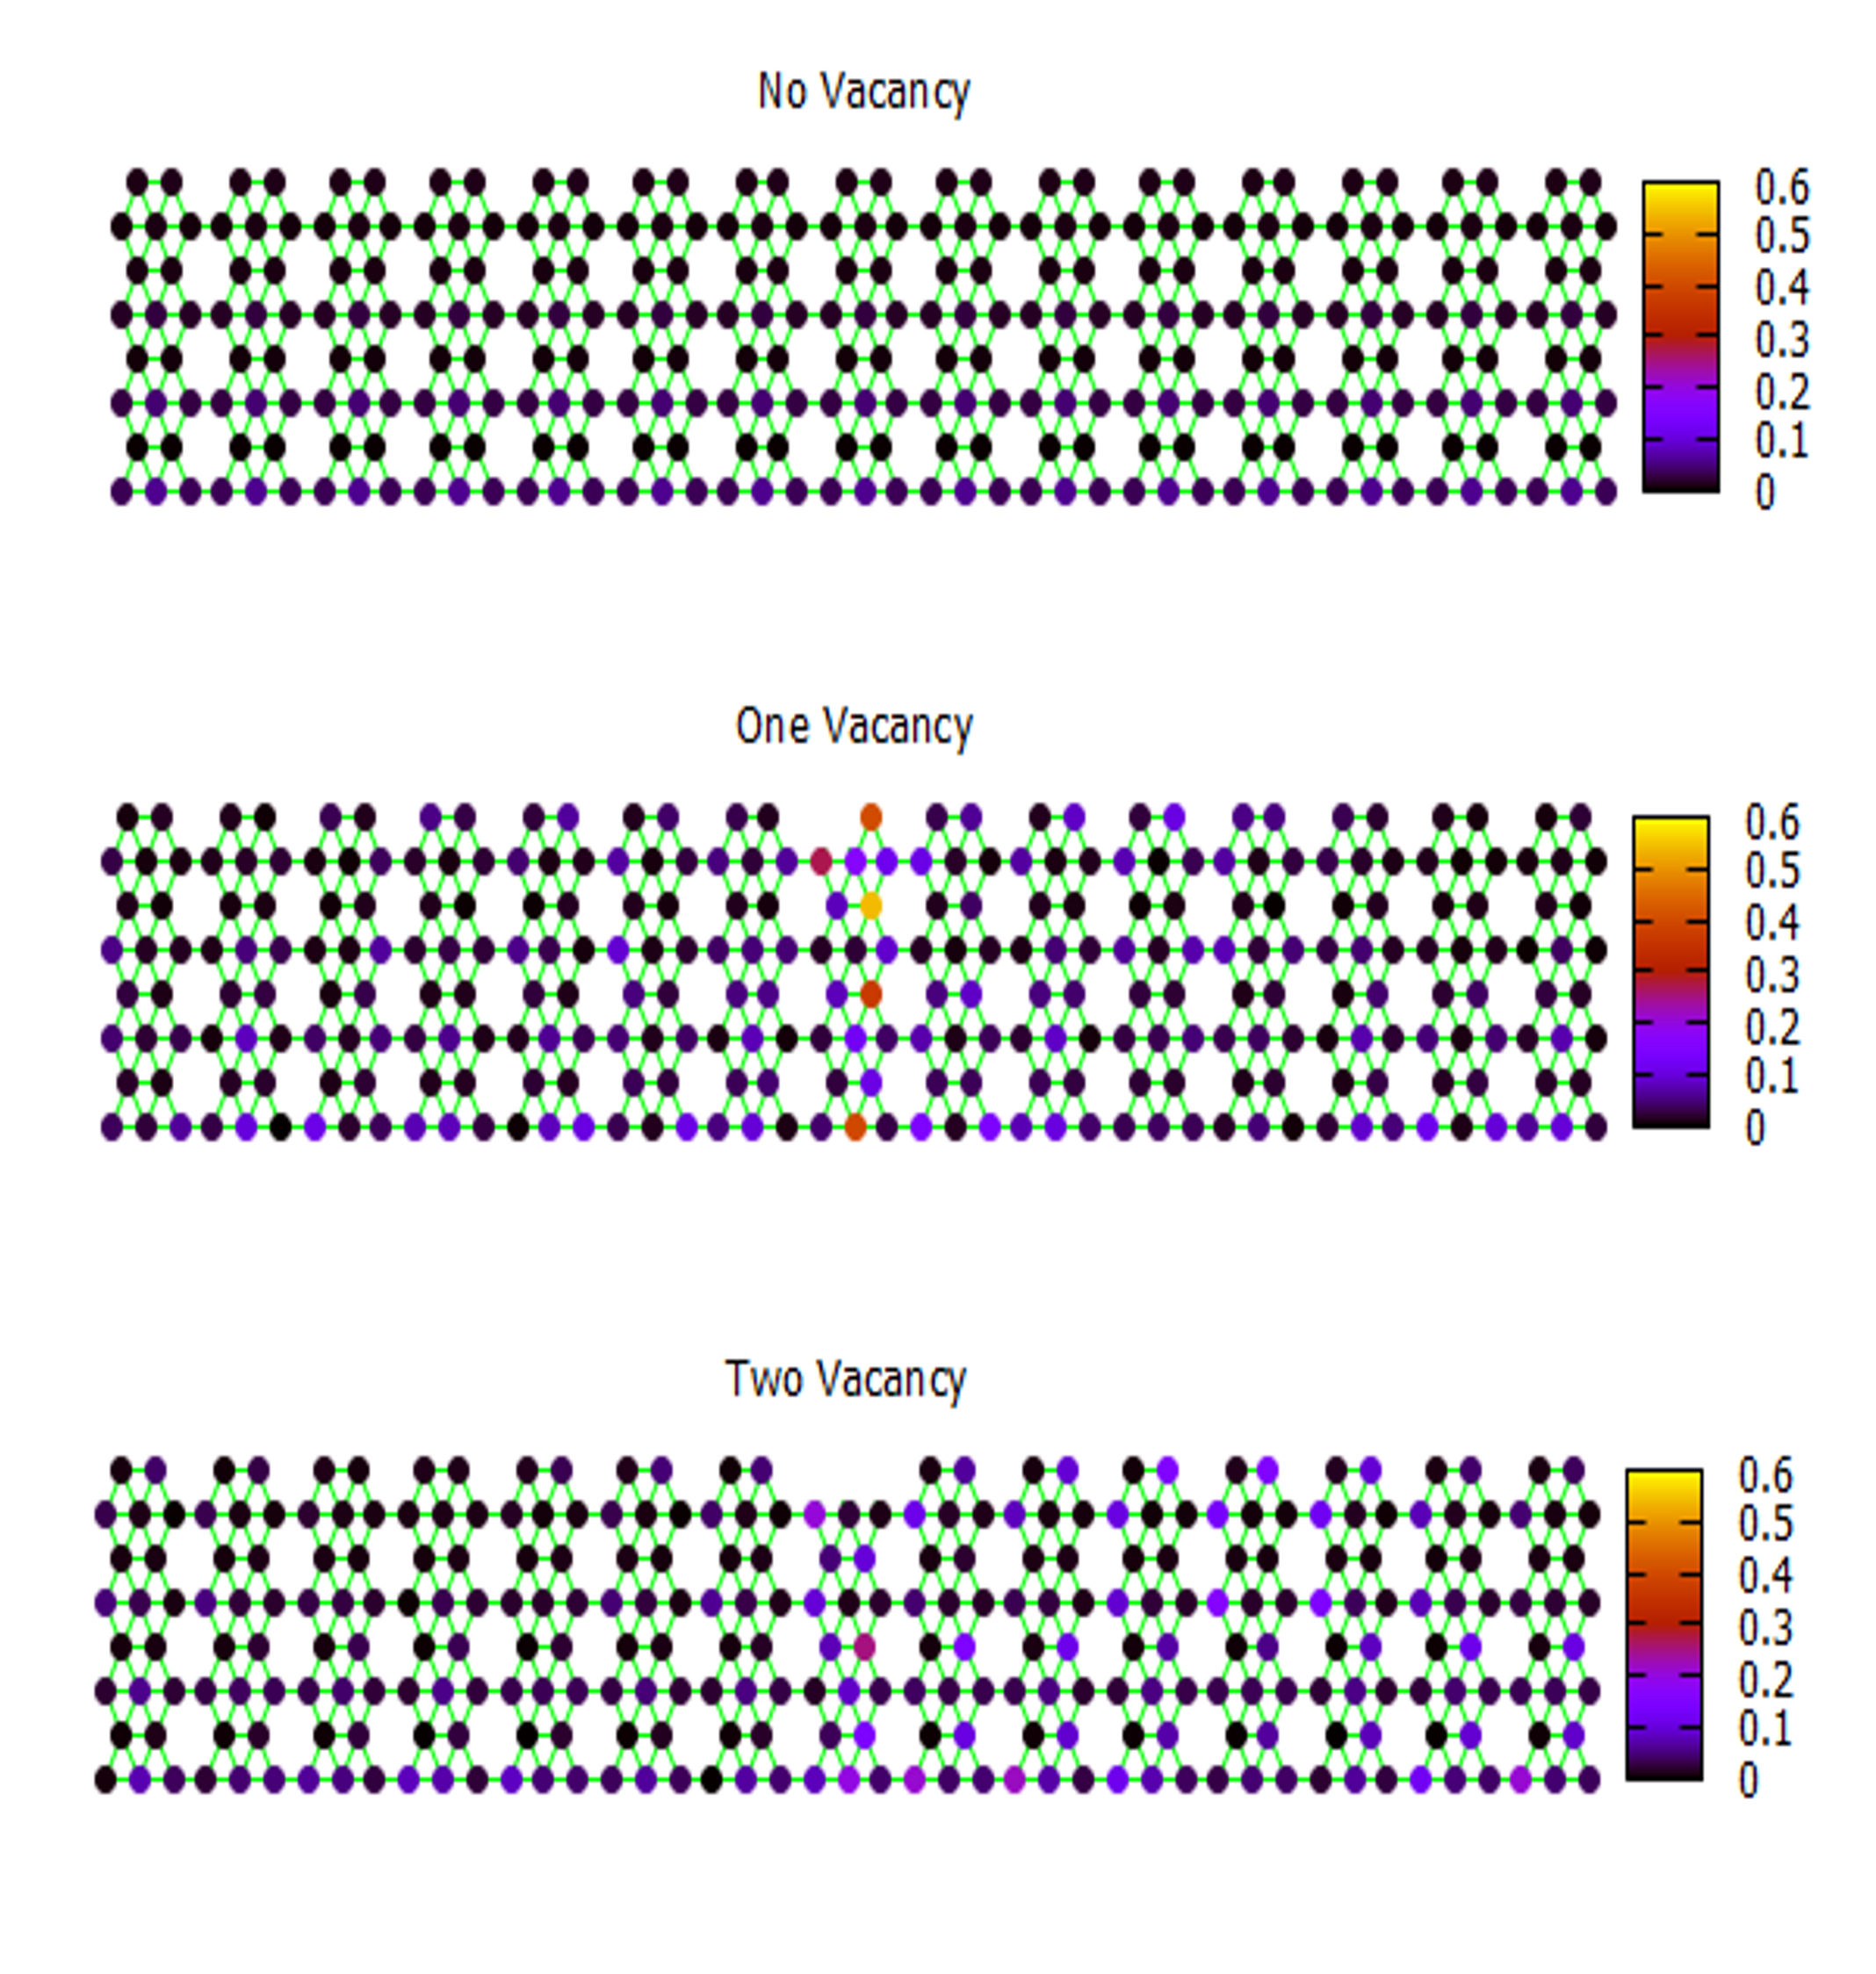
\includegraphics[width=1\linewidth]{./figures/Slide5.PNG}
\caption{در انرژی مربوط به اوج \lr{LDOS} در نزدیکی انرژی فر‌می‌، چگالی الکترونی فضایی حالات در کل محل نانوروبان ‌بورفین آرمچیر با یک محل خالی در لبه بالایی خالی، یک جای خالی، و دو جای خالی در وسط رسم شد. از نانو روبان}
\label{armVSLDOS}
\end{figure}
%%%% بنظر ‌می‌رسد داشتن یک تصویر شماتیک برای این مبحث ضروری است که از مقاله واکی بایاشی بایدگرفت
در اینجا جهت تغییر ناپذیر انتقالی محور زیگزاگ را به عنوان محور \lr{x} و محور \lr{y} را عمود بر محور x در نظر ‌‌می‌‌گیریم. این انتگرال عموماً یک عدد مختلط است، به این معنی که حالت کران تشدید ‌‌می‌‌شود، یا به عبارت دیگر، یک حالت کران مجازی وجود دارد. برای نوارهای آرمچیر با عرض \lr{\AA}18.59 و با بی‌نظ‌‌می‌‌ توزیع شده در هر دو لبه در طول \lr{\AA}758.81 با اختلال نسبتاً ضعیف $V_d = 1 eV$، \gls{BNR}‌های آرمچیر از فلز به نیمه‌هادی تبدیل ‌‌می‌‌شوند. با یک عمر محدود در حد پتانسیل نامتناهی \lr{V} (یعنی یک جای خالی واحد در \gls{BNR}ها)، حالت کران مجازی به یک حالت کران کاملاً تعریف شده تبدیل ‌‌می‌‌شود (با طول عمر نامحدود)، و سطح انرژی ناخالصی در $E = 0$ رخ ‌‌می‌‌دهد. معادله شرودینگر را ‌می‌‌توان برای به دست آوردن حالت ویژه در فضای \lr{k} با استفاده از این واقعیت که چگالی حالات برای یک سیستم دوبعدی با انرژی متناسب است استفاده کرد:
\begin{subequations}
  \begin{eqnarray}
    \phi_{Ak}&=\frac{V}{L^2}G_A^0\frac{E}{E^2-|\epsilon_k|^2},\\
    \phi_{Bk}&=\frac{V}{L^2}G_A^0\frac{\color{yellow}{\epsilon_k}}{E^2-|\epsilon_k|^2},
  \end{eqnarray}
  \label{}
  \end{subequations}
که در آن $G^0_A =\Sigma_k \phi_{Ak}$ با نرمال کردن توابع موج، متوجه ‌‌می‌‌شویم که آنها دارای ویژگی غیرمحدود هستند، به عنوان مثال $\phi_{A}(r) = 0$ و $\phi_{B}(r)\neq 0$. بنابراین، هنگا‌‌می‌‌ که یک جای خالی روی شبکه لانه زنبوری ایجاد ‌‌می‌‌شود، سطح انرژی جای خالی در $E = 0$ با تابع موجی ظاهر ‌‌می‌‌شود که دارای یک کاراکتر غیرمحدود است، یعنی دامنه آن در سایت \lr{a(b)} صفر است. همانطور که با معادله\ref{virtual} مشاهده ‌‌می‌‌شود، وجود جاهای خالی باعث سطح انرژی $E = 0$ ‌‌می‌‌شود. از سوی دیگر، نشان داده شده است که حالت‌های لبه فقط در نانوروبان‌های زیگزاگ وجود دارد و نه در آرمچیر. مشخص شده است که حالت‌های لبه را ‌‌می‌‌توان به ترتیب در شکاف نوار یا شکاف نوار جایگزیده در نیمه‌هادی‌ها و‌هادی‌ها نیز یافت \cite{breyElectronicStatesGraphene2006}. علاوه بر این، در نانوروبان‌های زیگزاگ، دو سطح انرژی در شکاف نوار وجود دارد که ‌می‌توانند با هم جفت شوند و باعث فرورفتگی رسانایی شوند، در حالی که برای نانوروبان‌های آرمچیر، هیچ جفت‌شدگیی وجود ندارد. انرژی این افت‌های رسانایی مطابق با پیکربندی‌های ضد پیوند \cite{wakabayashiELECTRICALCONDUCTANCEZIGZAG2002} است. بر اساس مدل فوق، اکنون ممکن است اثر یک نقص را بر رسانایی یک \gls{BNR} به صورت کمی‌‌ بررسی کنیم. محاسبات عددی ما \gls{LDOS} تقریباً صفر را در محل پراکندگی نشان ‌می‌دهد، که مربوط به کاراکتر نامحدود مدل مورد بررسی است. شکل\ref{zigvacancy}(الف) رسانایی نانوروبان‌های زیگزاگی با عرض \lr{\AA} 18.59 و طول \lr{\AA}42.34 (15 سوپرسل) را نشان ‌‌می‌‌دهد، زمانی که یک ناخالصی با انواع قدرت‌های بالقوه در لبه بالایی سوپرسل واقع در وسط نانو نوار وجود دارد. در شکل\ref{zigvacancy}، \gls{LDOS} در نزدیکترین محل ناخالصی همسایه مانند بالا رسم شده است. همانطور که انتظار داریم، وجود ناخالصی باعث کاهش رسانایی ‌‌می‌‌شود به طوری که در انرژی‌های خاص منجر به افت رسانایی ‌‌می‌‌شود که به طور معادل با پیک در \gls{LDOS} همراه است. همانطور که قبلا ذکر شد، یک شبکه لانه زنبوری پنهان در شبکه ‌بورفین $\beta_{12}$ وجود دارد، بنابراین افت رسانایی، همراه با قله‌های \gls{LDOS}، ‌‌می‌‌تواند به حالت‌های شبه موضعی که در مجاورت ناخالصی رخ ‌‌می‌‌دهد نسبت داد
% \subsection{چگالی حالت‌های فضایی}
در این رساله، رسانایی نانوروبان‌های 
آزمایش‌ها و\gls{محاسبات اصول اولیه} نشان داده‌اند که مخروطهای دیراک از اوربیتال‌های $P_z$ مشتق شده‌اند. از آنجایی که تابع موج در انرژی فر‌‌می‌‌ در محل \lr{c} دامنه ندارد، \cite{fengDiracFermionsBorophene2017} این شش اتم اطراف فاز یکدیگر را خنثی ‌‌می‌‌کنند، بنابراین شکل\ref{zigCSLDOS} در انرژی متناظر تا اوج \gls{LDOS} در نزدیکی انرژی فر‌می‌، چگالی الکترونی فضایی حالتها در کل محل نانوروبان ‌بورفین زیگزاگ با محل پراکندگی در لبه بالایی با \lr{V=0,1,2,5} در وسط نانوروبان ترسیم شده است. 

\begin{figure}[!ht]
  \centering
  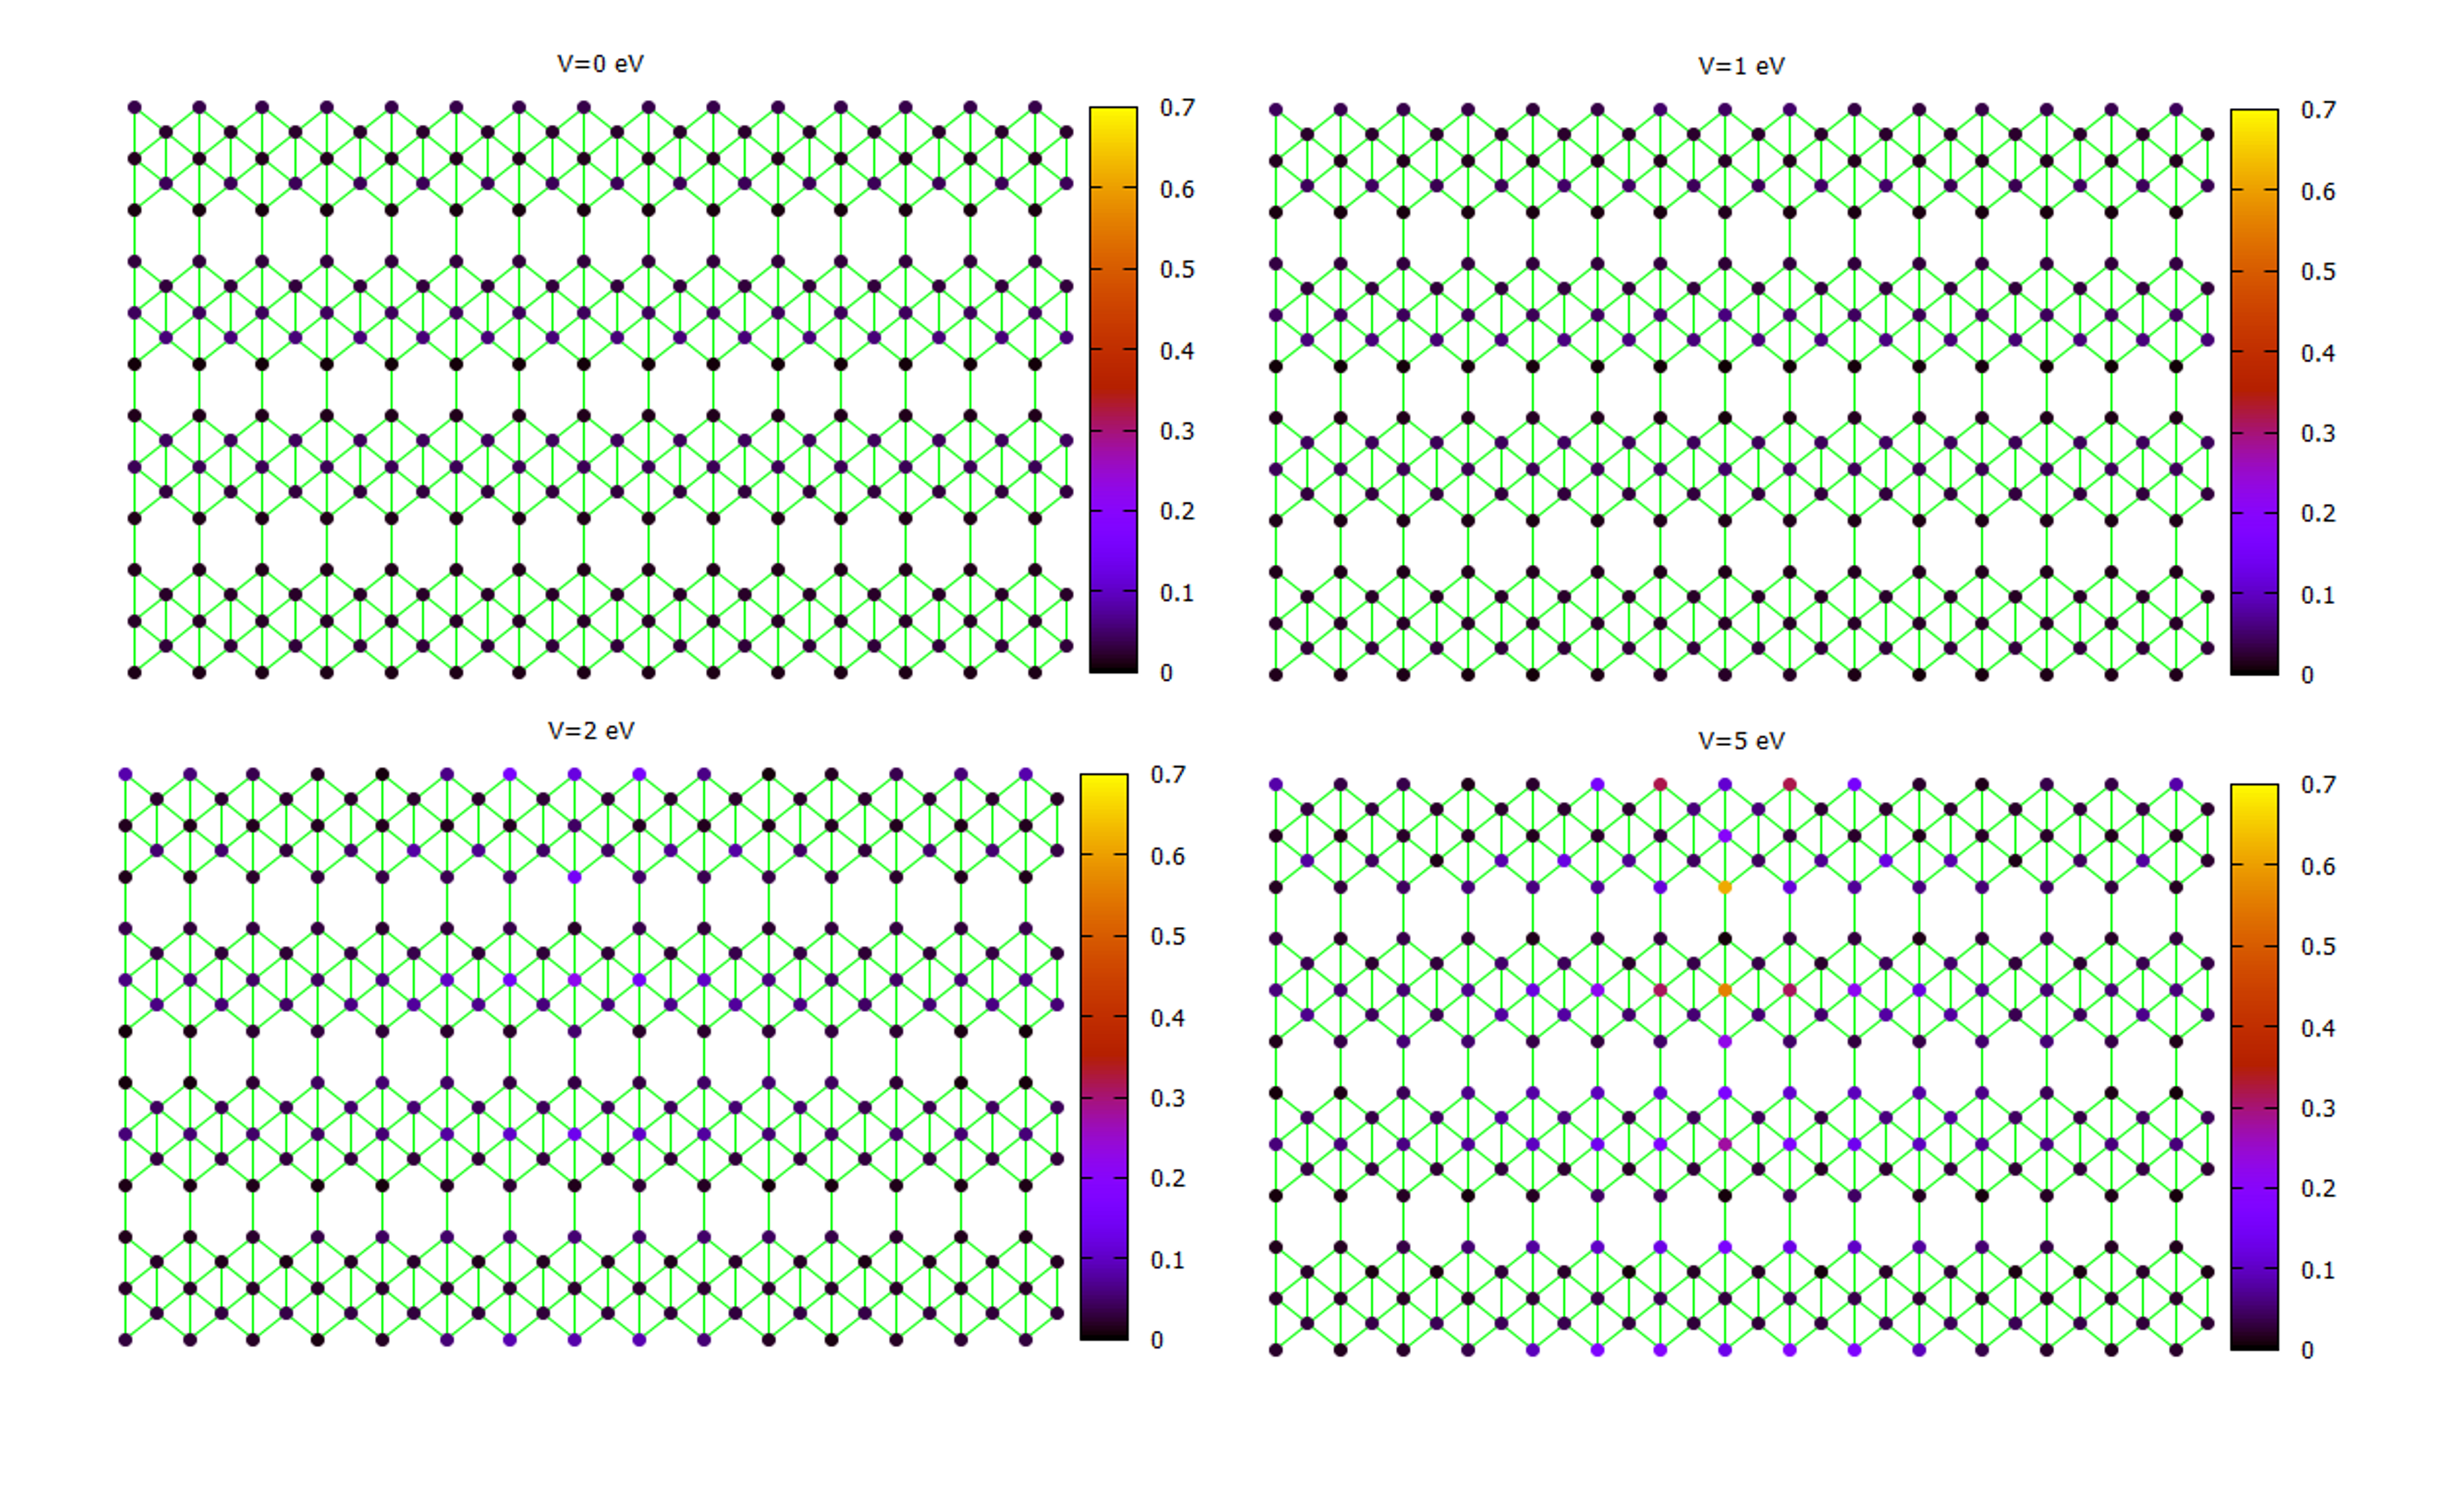
\includegraphics[width=1\linewidth]{./figures/Slide1.PNG}
  \caption{در انرژی مربوط به اوج \gls{LDOS} نزدیک انرژی فر‌می‌، چگالی الکترونی فضایی حالات در کل محل نانوروبان ‌بورفین زیگزاگ با یک محل پراکندگی در لبه بالایی با \lr{V=0،1،2،5} در وسط رسم شد. از نانو روبان}
  \label{zigCSLDOS}
\end{figure}

\begin{figure}[!ht]
  \centering
  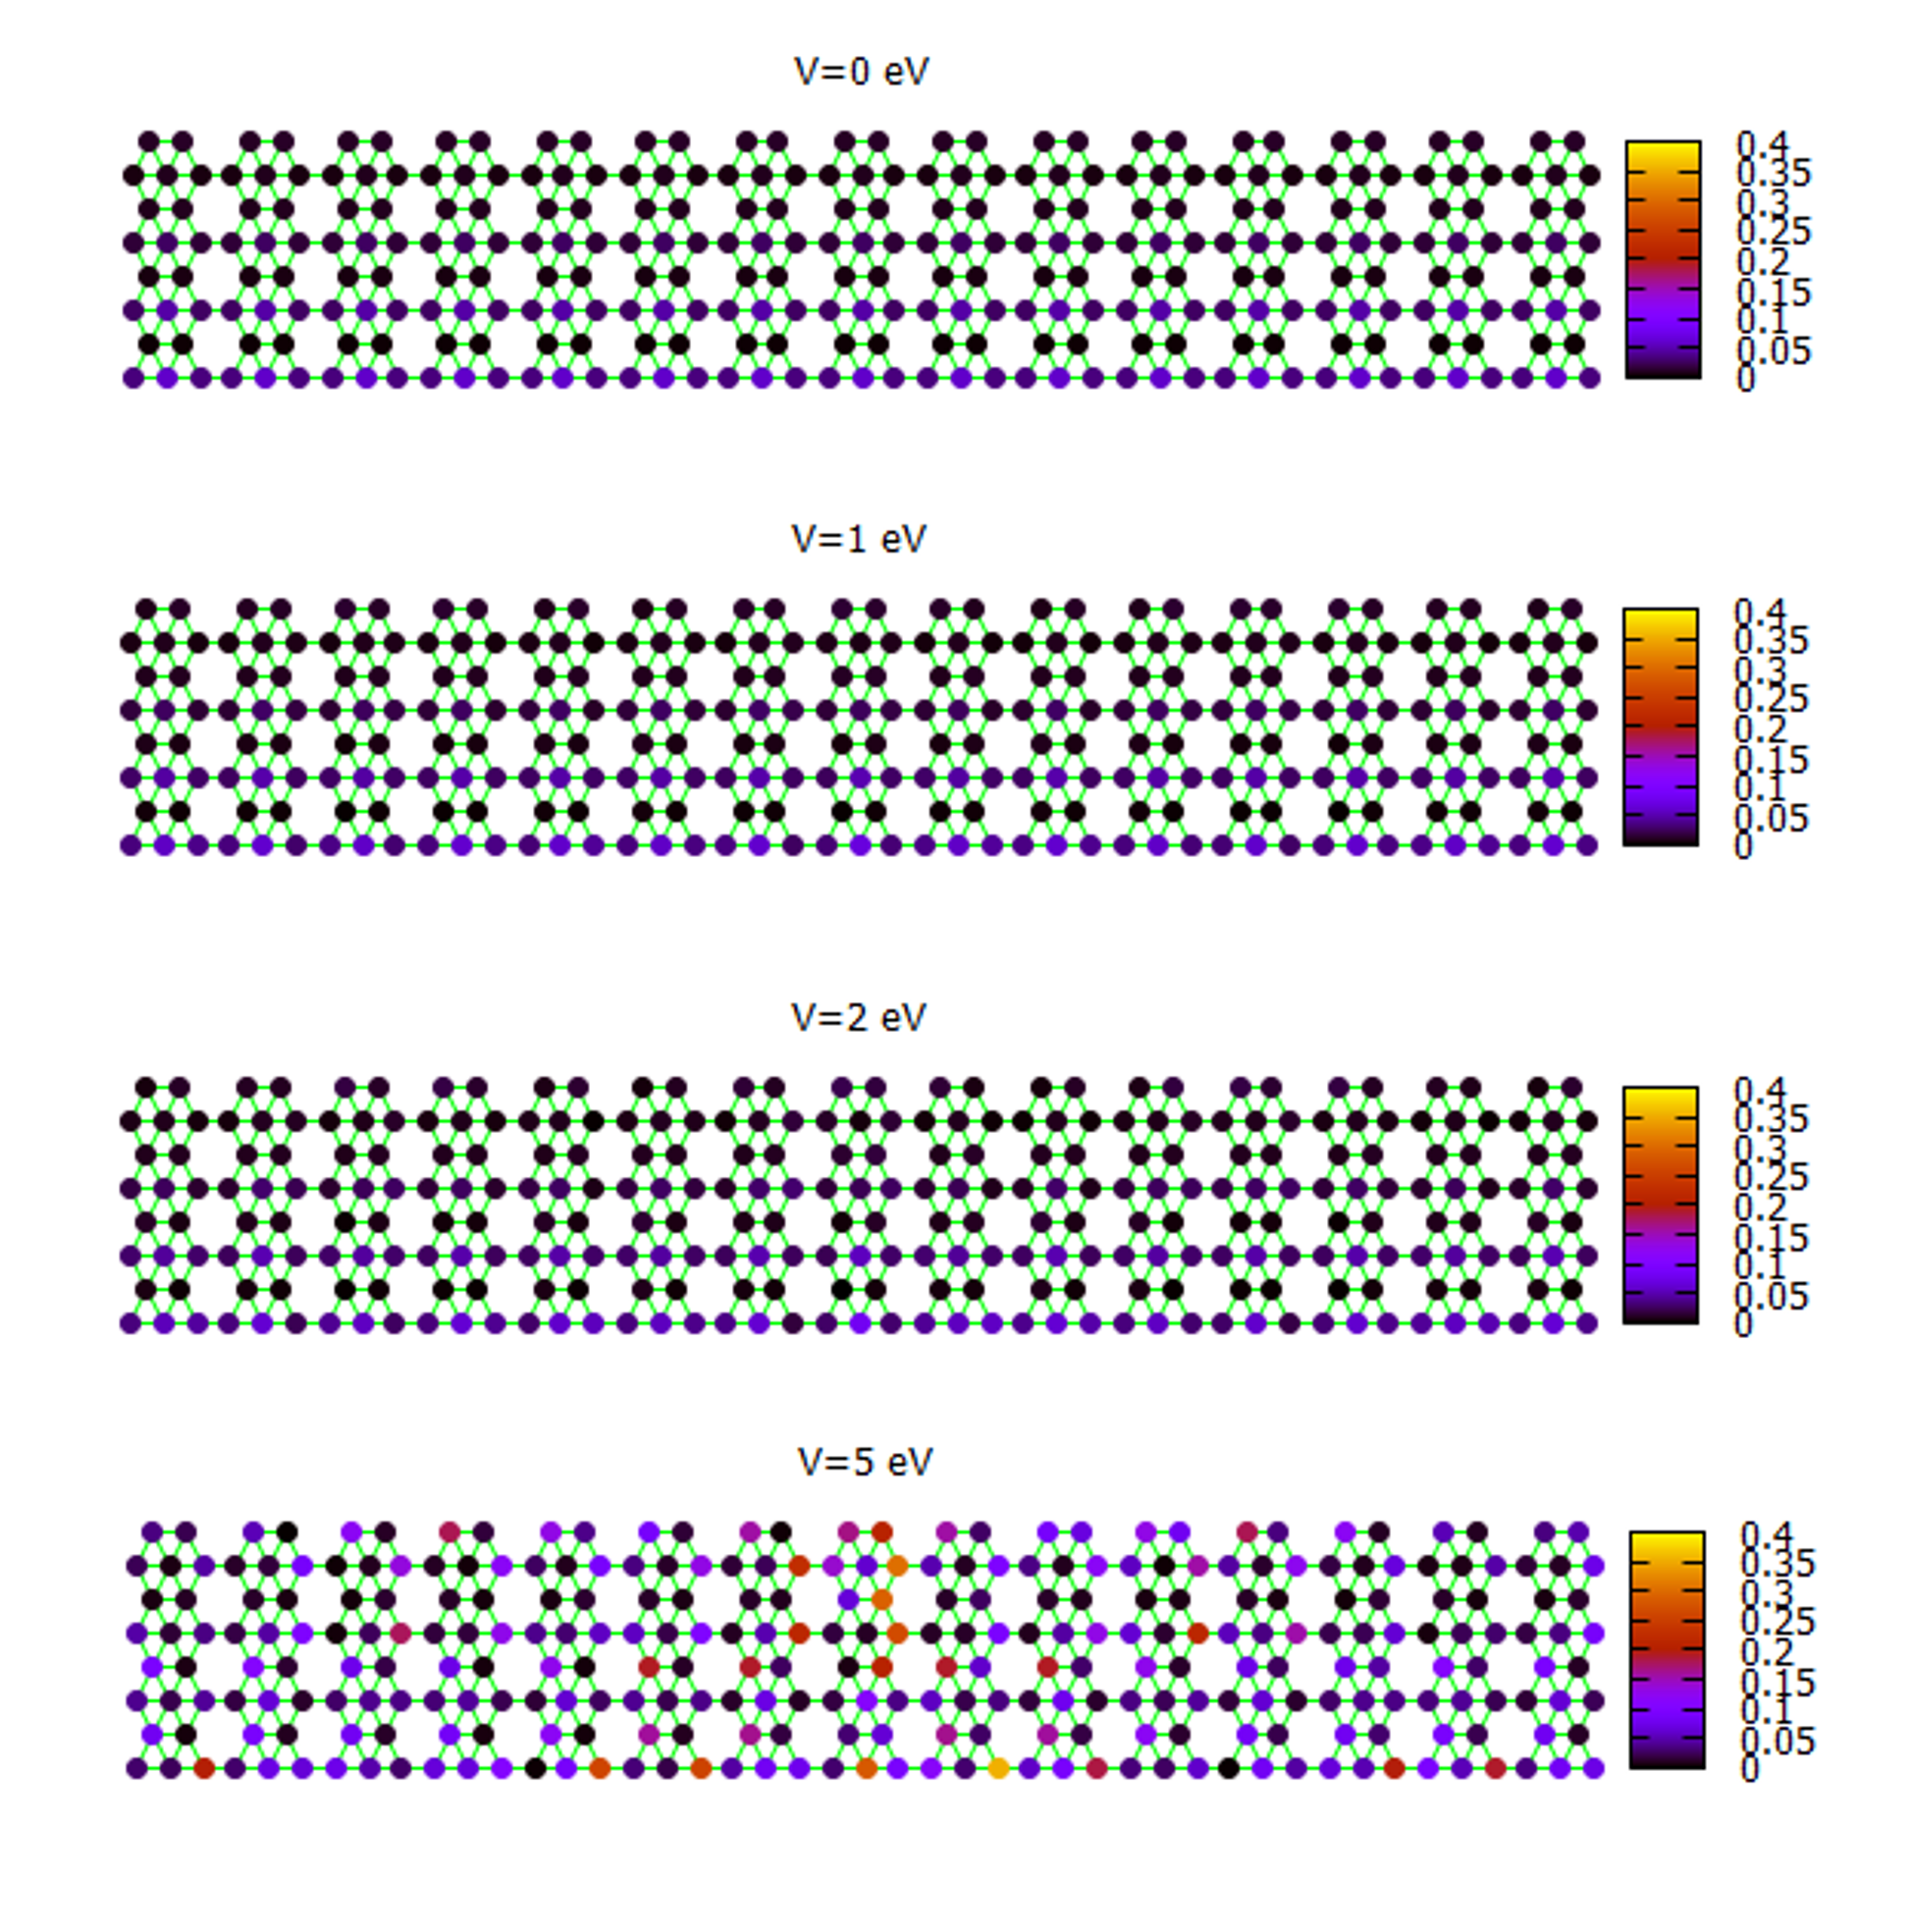
\includegraphics[width=1\linewidth]{./figures/Slide3.PNG}
  \caption{در انرژی مربوط به اوج \gls{LDOS} نزدیک انرژی فر‌می‌، چگالی الکترونی فضایی حالات در کل محل نانوروبان ‌بورفین آرمچیر با یک محل پراکندگی در لبه بالایی با \lr{V=0،1،2،5} در وسط رسم شد. از نانو روبان}
  \label{armCSLDOS}
\end{figure}
\begin{figure}[!ht]
    \centering
    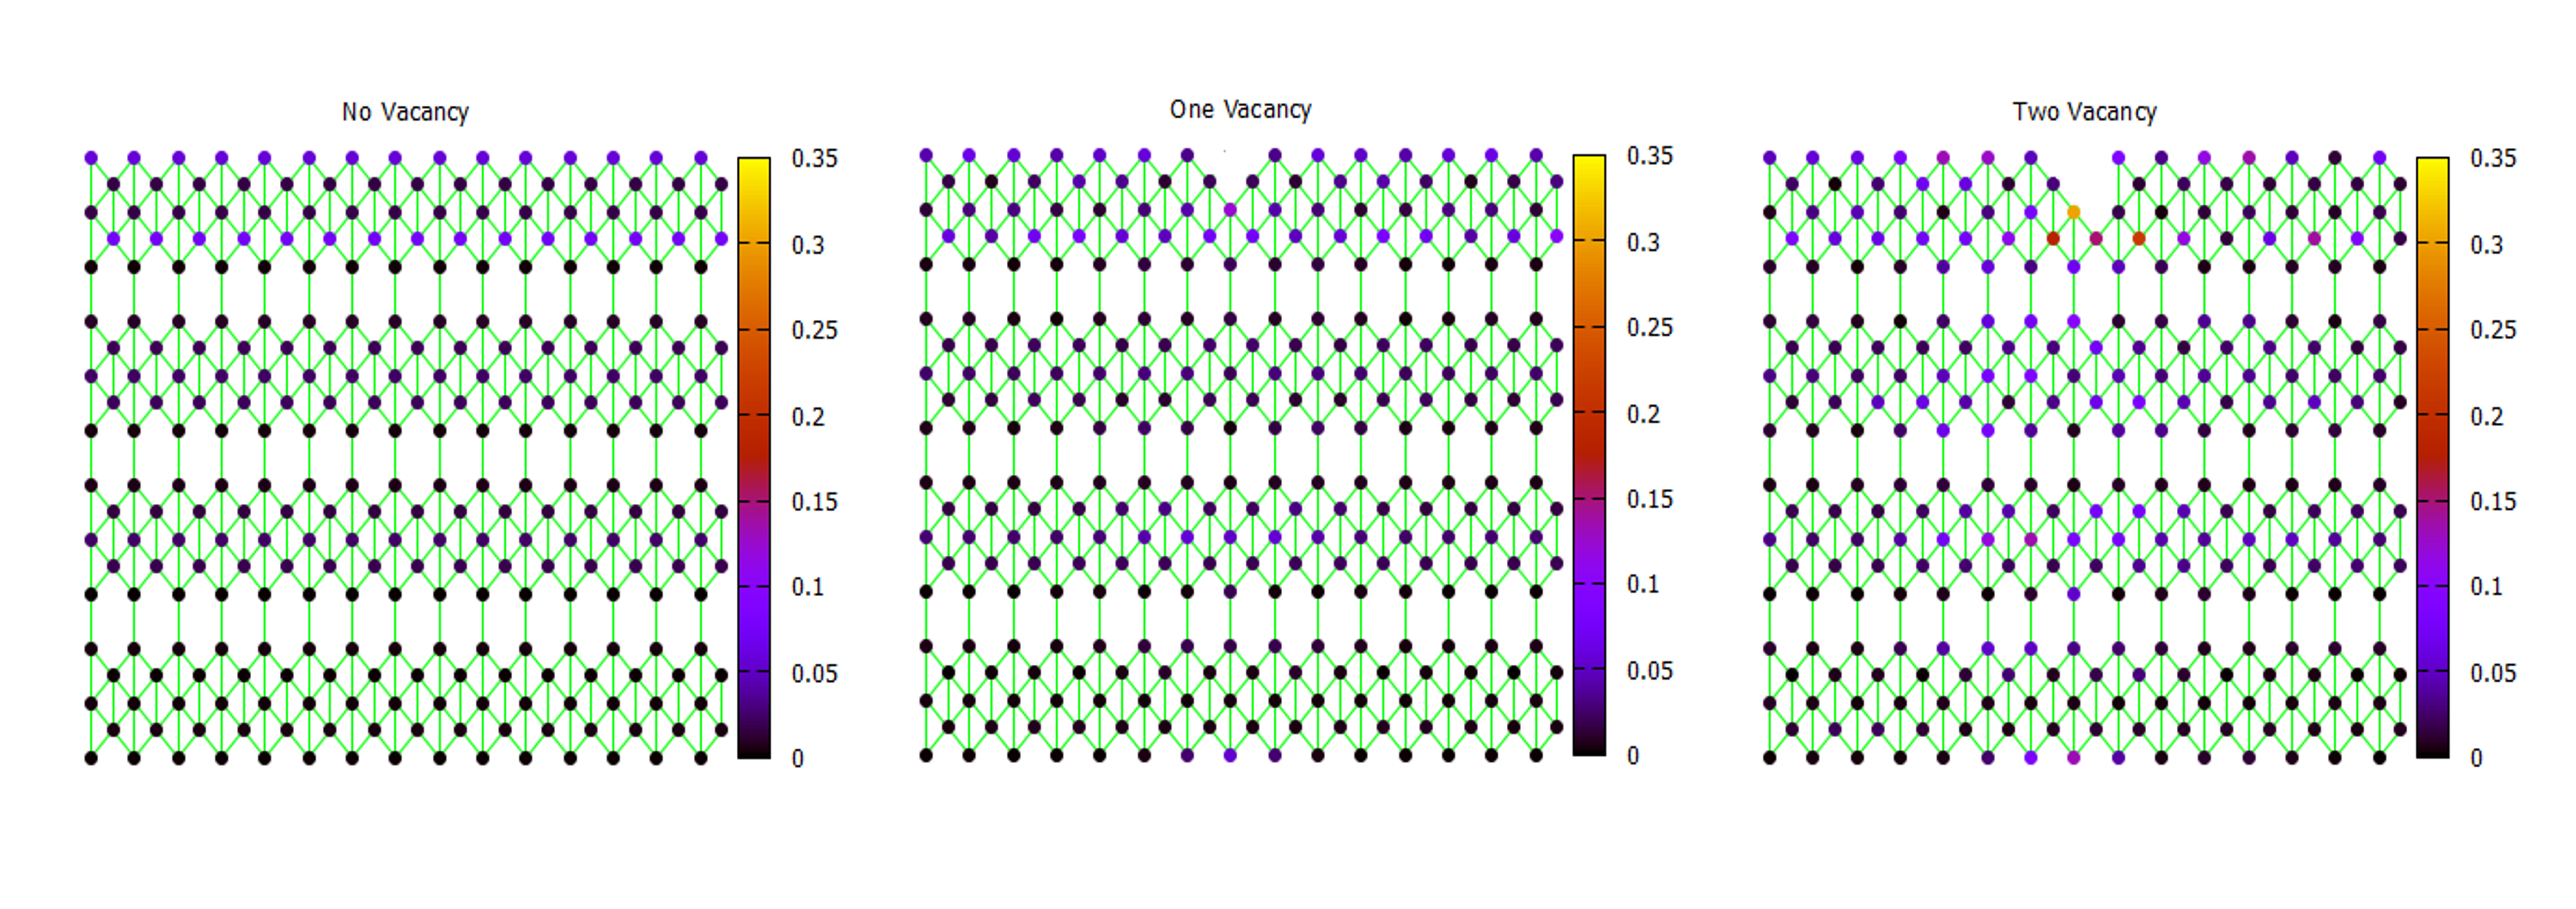
\includegraphics[width=1\linewidth]{./figures/Slide4.PNG}
    \caption{در انرژی مربوط به اوج \gls{LDOS} در نزدیکی انرژی فر‌می‌، چگالی الکترونی فضایی حالت‌ها در کل محل نانوروبان ‌بورفین زیگزاگ با یک محل خالی در لبه بالایی خالی، یک جای خالی و دو جای خالی در وسط رسم شد. از نانو روبان}
    \label{zigVSLDOS}
\end{figure}
\begin{figure}[!ht]
\centering
% GNUPLOT: LaTeX picture with Postscript
\begingroup
  % Encoding inside the plot.  In the header of your document, this encoding
  % should to defined, e.g., by using
  % \usepackage[cp1252,<other encodings>]{inputenc}
  % \inputencoding{cp1252}%
  \makeatletter
  \providecommand\color[2][]{%
    \GenericError{(gnuplot) \space\space\space\@spaces}{%
      Package color not loaded in conjunction with
      terminal option `colourtext'%
    }{See the gnuplot documentation for explanation.%
    }{Either use 'blacktext' in gnuplot or load the package
      color.sty in LaTeX.}%
    \renewcommand\color[2][]{}%
  }%
  \providecommand\includegraphics[2][]{%
    \GenericError{(gnuplot) \space\space\space\@spaces}{%
      Package graphicx or graphics not loaded%
    }{See the gnuplot documentation for explanation.%
    }{The gnuplot epslatex terminal needs graphicx.sty or graphics.sty.}%
    \renewcommand\includegraphics[2][]{}%
  }%
  \providecommand\rotatebox[2]{#2}%
  \@ifundefined{ifGPcolor}{%
    \newif\ifGPcolor
    \GPcolorfalse
  }{}%
  \@ifundefined{ifGPblacktext}{%
    \newif\ifGPblacktext
    \GPblacktexttrue
  }{}%
  % define a \g@addto@macro without @ in the name:
  \let\gplgaddtomacro\g@addto@macro
  % define empty templates for all commands taking text:
  \gdef\gplbacktext{}%
  \gdef\gplfronttext{}%
  \makeatother
  \ifGPblacktext
    % no textcolor at all
    \def\colorrgb#1{}%
    \def\colorgray#1{}%
  \else
    % gray or color?
    \ifGPcolor
      \def\colorrgb#1{\color[rgb]{#1}}%
      \def\colorgray#1{\color[gray]{#1}}%
      \expandafter\def\csname LTw\endcsname{\color{white}}%
      \expandafter\def\csname LTb\endcsname{\color{black}}%
      \expandafter\def\csname LTa\endcsname{\color{black}}%
      \expandafter\def\csname LT0\endcsname{\color[rgb]{1,0,0}}%
      \expandafter\def\csname LT1\endcsname{\color[rgb]{0,1,0}}%
      \expandafter\def\csname LT2\endcsname{\color[rgb]{0,0,1}}%
      \expandafter\def\csname LT3\endcsname{\color[rgb]{1,0,1}}%
      \expandafter\def\csname LT4\endcsname{\color[rgb]{0,1,1}}%
      \expandafter\def\csname LT5\endcsname{\color[rgb]{1,1,0}}%
      \expandafter\def\csname LT6\endcsname{\color[rgb]{0,0,0}}%
      \expandafter\def\csname LT7\endcsname{\color[rgb]{1,0.3,0}}%
      \expandafter\def\csname LT8\endcsname{\color[rgb]{0.5,0.5,0.5}}%
    \else
      % gray
      \def\colorrgb#1{\color{black}}%
      \def\colorgray#1{\color[gray]{#1}}%
      \expandafter\def\csname LTw\endcsname{\color{white}}%
      \expandafter\def\csname LTb\endcsname{\color{black}}%
      \expandafter\def\csname LTa\endcsname{\color{black}}%
      \expandafter\def\csname LT0\endcsname{\color{black}}%
      \expandafter\def\csname LT1\endcsname{\color{black}}%
      \expandafter\def\csname LT2\endcsname{\color{black}}%
      \expandafter\def\csname LT3\endcsname{\color{black}}%
      \expandafter\def\csname LT4\endcsname{\color{black}}%
      \expandafter\def\csname LT5\endcsname{\color{black}}%
      \expandafter\def\csname LT6\endcsname{\color{black}}%
      \expandafter\def\csname LT7\endcsname{\color{black}}%
      \expandafter\def\csname LT8\endcsname{\color{black}}%
    \fi
  \fi
    \setlength{\unitlength}{0.0500bp}%
    \ifx\gptboxheight\undefined%
      \newlength{\gptboxheight}%
      \newlength{\gptboxwidth}%
      \newsavebox{\gptboxtext}%
    \fi%
    \setlength{\fboxrule}{0.5pt}%
    \setlength{\fboxsep}{1pt}%
\begin{picture}(5040.00,4320.00)%
    \gplgaddtomacro\gplbacktext{%
      \csname LTb\endcsname%%
      \put(550,704){\makebox(0,0)[r]{\strut{}$0$}}%
      \put(550,1128){\makebox(0,0)[r]{\strut{}$1$}}%
      \put(550,1553){\makebox(0,0)[r]{\strut{}$2$}}%
      \put(550,1977){\makebox(0,0)[r]{\strut{}$3$}}%
      \put(550,2402){\makebox(0,0)[r]{\strut{}$4$}}%
      \put(550,2826){\makebox(0,0)[r]{\strut{}$5$}}%
      \put(550,3250){\makebox(0,0)[r]{\strut{}$6$}}%
      \put(550,3675){\makebox(0,0)[r]{\strut{}$7$}}%
      \put(550,4099){\makebox(0,0)[r]{\strut{}$8$}}%
      \put(682,484){\makebox(0,0){\strut{}$-2$}}%
      \put(1177,484){\makebox(0,0){\strut{}$-1.5$}}%
      \put(1672,484){\makebox(0,0){\strut{}$-1$}}%
      \put(2167,484){\makebox(0,0){\strut{}$-0.5$}}%
      \put(2663,484){\makebox(0,0){\strut{}$0$}}%
      \put(3158,484){\makebox(0,0){\strut{}$0.5$}}%
      \put(3653,484){\makebox(0,0){\strut{}$1$}}%
      \put(4148,484){\makebox(0,0){\strut{}$1.5$}}%
      \put(4643,484){\makebox(0,0){\strut{}$2$}}%
    }%
    \gplgaddtomacro\gplfronttext{%
      \csname LTb\endcsname%%
      \put(198,2401){\rotatebox{-270}{\makebox(0,0){\strut{}$G/G_0$}}}%
      \put(2662,154){\makebox(0,0){\strut{}Energy(eV)}}%
      \csname LTb\endcsname%%
      \put(3656,3926){\makebox(0,0)[r]{\strut{}pristine ZBNR}}%
      \csname LTb\endcsname%%
      \put(3656,3706){\makebox(0,0)[r]{\strut{}V=0.25 eV}}%
      \csname LTb\endcsname%%
      \put(3656,3486){\makebox(0,0)[r]{\strut{}V=0.5 eV}}%
      \csname LTb\endcsname%%
      \put(3656,3266){\makebox(0,0)[r]{\strut{}V=2 eV}}%
    }%
    \gplbacktext
    \put(0,0){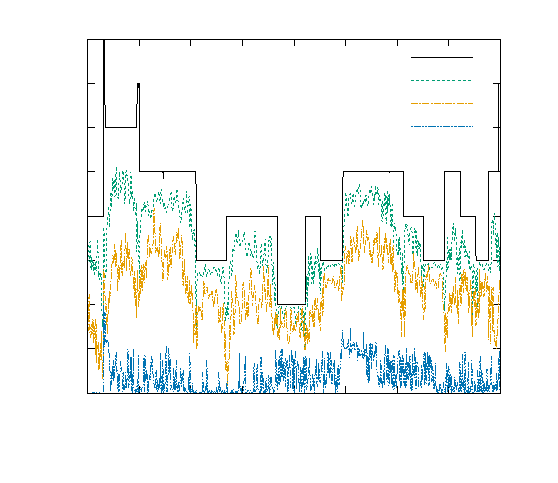
\includegraphics[width={253.00bp},height={217.00bp}]{zigzagdisorder}}%
    \gplfronttext
  \end{picture}%
\endgroup

\caption{رسانایی در مقابل انرژی برای نوارهای زیگزاگی با عرض \lr{\AA} 10.24 و با بی نظ‌‌می‌‌ در هر دو لبه به طول \lr{\AA} 876.68 توزیع شده است
با یک اختلال نسبتا ضعیف $V_d=2\;eV$، \gls{BNR}‌های زیگزاگی از فلز به نیمه‌هادی تبدیل ‌‌می‌‌شوند.}
\label{zigzagdisorder}
\end{figure}
توزیع چگالی حالت‌ها در همه مکان‌های نانوروبان به انرژی بستگی دارد. توزیع چگالی حالت‌ها حول $E=-0.034$ ترسیم شده است در شکل\ref{zigCSLDOS}. شکل\ref{zigCSLDOS} نشان ‌‌می‌‌دهد که در حالی که هیچ پراکنده‌ای روی نانوروبان وجود ندارد، توزیع چگالی حالت‌ها تقریباً در همه مکان‌ها برابر است. با قرار دادن پراکنده در لبه بالایی سوپرسل ‌میانی نانوروبان معادل شکل\ref{fig:borophene}، توزیع چگالی حالت‌ها در اطراف ابرسلول ‌میانی افزایش ‌‌می‌‌یابد. با افزایش قدرت پراکندگی، چگالی حالات در اطراف ابرسلول مرکزی افزایش ‌‌می‌‌یابد. با افزایش قدرت پراکنده، توزیع چگالی حالت‌ها به سمت نزدیکترین محل به پراکنده مشهود است. در شکل\ref{armscatter}(الف) و شکل \ref{armscatter}(ب)،رسانایی و \gls{LDOS} به ترتیب برای \gls{ABNR}ها با عرض \lr{\AA} 10.24 رسم شده است. ناخالصی در لبه بالایی سوپرسل ‌میانی نانوروبان قرار دارد. در هر دو \gls{BNR} آرمچیر و زیگزاگ، ناخالصی‌های ضعیف ن‌‌می‌‌توانند بر رسانایی تأثیر بگذارند. با این حال، با افزایش قدرت پتانسیل ناخالصی‌ها، شیب رسانایی در اطراف انرژی فر‌‌می‌‌ همزمان با پیک \gls{LDOS} در محل مجاور ناخالصی ایجاد ‌‌می‌‌شود. بنابراین حالت‌های شبه موضعی را ‌‌می‌‌توان در ناخالصی‌های قوی مشاهده کرد. در \gls{ZBNR}ها، فرورفتگی‌های رسانایی، در نتیجه ناخالصی لبه، به وضوح در لبه نوار مشاهده ‌‌می‌‌شود، و عرض شیب‌ها زمانی که قدرت پتانسیل نقص مشاهده ‌‌می‌‌شود، قابل توجه ‌‌می‌‌شود. بیشتر از $2 eV$ با این حال، در \gls{ABNR} ها، یک شیب رسانایی در اطراف انرژی فر‌‌می‌‌ ظاهر ‌‌می‌‌شود، جایی که یک پیک معادل، مرتبط با حالت‌های شبه موضعی را ‌‌می‌‌توان در LDOS مشاهده کرد، زمانی که نقص قدرت بالقوه $5 eV$ باشد. شکل \ref{armCSLDOS} افزایش چگالی حالت‌ها را در اطراف سوپرسل ‌میانی نانوروبان با لبه‌های آرمچیر با انرژی $0.19\; eV$ نشان ‌‌می‌‌دهد. علاوه بر این، نشان ‌‌می‌‌دهد که یک پراکنده روی لبه ‌بورفین با لبه آرمچیر دارای تأثیر بیشتری نسبت به یک پراکنده روی لبه ‌بورفین با لبه زیگزاگ است. بنابراین این موضوع مقایسه رسانایی و \gls{LDOS} در شکل \ref{zigscatter} و \ref{armscatter} را تایید ‌‌می‌‌کند که اثر پراکندگی بر روی رسانایی و نمودار \gls{LDOS} ‌بورفین با لبه آرمچیر قابل توجه‌تر است. در شکل \ref{armvacancy}، رسانایی و \gls{LDOS} مربوطه برای \gls{ABNR}ها با عرض \lr{\AA} 10.24 (4 سلول واحد در سوپرسل) در دو حالت خالی، یک یا دو اتم خالی ترسیم شده است. تأثیر جای خالی لبه تک  اتمی‌‌ و جای خالی لبه دواتمی‌‌ بر رسانایی \gls{ABNR}ها کاملاً متفاوت است. در حالت اول، فرورفتگی‌های رسانایی در لبه‌های نوارها ظاهر ‌می‌شوند، که متفاوت از تکینگی‌های \gls{Van-Hoff} سیستم خالص است، بنابراین شواهدی مبنی بر وجود شبه ذرات در آن انرژی وجود دارد. قبلاً دیده شده است که یک شبکه لانه زنبوری پنهان در ساختار شبکه $\beta_{12}$ وجود دارد و متعاقباً مشابه گرافین، ممکن است دو زیرشبکه تعریف شود. در نتیجه، شیب رسانایی برجسته در دو‌می‌، که با یک قله بزرگ در \gls{LDOS} در انرژی فر‌‌می‌‌ همراه است، از شکستن تقارن زیرشبکه نشات ‌می‌گیرد. همانطور که قبلا ذکر کردیم، در حالی که قدرت پراکندگی را تا بی نهایت افزایش ‌‌می‌‌دهیم، به نانوروبان با یک جای خالی در لبه ‌‌می‌‌رسیم. بنابراین، چگالی حالت‌ها در اطراف سوپرسل ‌میانی دارای بیشترین غلظت و تقریباً مقدار قابل توجهی \gls{LDOS} است که در نزدیکترین مکان به جای خالی قرار ‌می‌گیرد. شکست تقارن انتقالی در حضور یک جای خالی در نانوروبان با لبه آرمچیر در شکل \ref{zigVSLDOS} مشاهده شده است و نتایج قبلی ذکر شده در شکل \ref{zigvacancy} را تایید ‌‌می‌‌کند. \gls{ZBNR}های با جای خالی لبه‌های رفتاری مشابه با جای خالی لبه‌های نانوروبان‌های گرافین آرمچیر راحتی دارند، زیرا فرورفتگی‌های رسانایی در لبه‌های نوارهای مربوط به قله‌های \gls{LDOS} رخ ‌می‌دهد تا حالت‌های شبه موضعی ممکن است نتیجه‌گیری شود. با این حال، در مورد جاهای خالی لبه دواتمی‌‌ در \gls{ZBNR}، یک شیب رسانایی بزرگ با یک \gls{LDOS} بزرگ معادل در انرژی فر‌‌می‌‌ دیده ‌می‌شود، مانند مورد \gls{ABNR}، که کاملاً با \gls{GNR}ها متناقض است. این را ‌‌می‌‌توان با شکستن تقارن توضیح داد. زیرشبکه به دلیل وجود اتم ‌میانی در سلول واحد در لبه. همچنین، در ‌بورفین با لبه زیگزاگ (شکل\ref{zigVSLDOS})، مانند \gls{ABNR}ها، حد نهایی \lr{LDOS} در نزدیکترین محل پراکنده نشان داده شده است و ‌‌می‌‌توان مشاهده کرد که نتایج قبلی به دست آمده از شکل \ref{zigvacancy} را تایید ‌‌می‌‌کند.
% چگالی الکترونی فضایی حالتها در کل محل نانوروبان ‌بورفین آرمچیر با یک مکان پراکندگی در لبه بالایی با \lr{V=0،1،2،5} در وسط نانوروبان ترسیم شده است. شکل\ref{zigvacancy}.

بورفین زیگزاگ و آرمچیر با نقص‌های منفرد و اختلالات ضعیف در لبه‌ها را در چارچوب مدل اتصال محکم با استفاده از تکنیک تابع گرین بررسی کرده‌ایم. رسانایی نانوروبان‌های ‌بورفین خالص رفتار گام به گام را نشان ‌می‌دهد و تعداد کانال‌های رسانایی در انرژی فر‌‌می‌‌ به عرض ‌بورفین بستگی دارد، به دلیل وجود اتم مرکزی در سلول واحد ‌بورفین، در تضاد واضح با مورد گرافین. ابتدا دو نوع نقص لبه را معرفی ‌می‌کنیم، یعنی نقص‌های منفرد شامل تک پراکندگی و تک خالی و اختلال ضعیف. نانوروبان‌های ‌بورفین زیگزاگ همگی رفتار فلزی از خود نشان ‌می‌دهند، در حالی که \gls{BNR}های آرمچیر راحتی بسته به عرض، رفتار فلزی یا نیمرسانا را نشان ‌می‌دهند. مشخص شده است که عیوب منفرد لبهای باعث حالت‌های شبه موضعی ‌می‌شوند و بنابراین افت رسانایی ظاهر ‌می‌شوند. بنابراین، این نتایج ممکن است وجود شبکه لانه زنبوری پنهان را در داخل یک $\beta_{12}$-‌بورفین با وجود ساختار شبکه مستطیلی آن تأیید کند. علاوه بر این، جای خالی یک  اتمی‌‌ و دو  اتمی‌‌ بر ترابرد الکترون‌ها به طور قابل توجهی نسبت به مورد قبلی از طریق تشکیل حالت‌های شبه موضعی و افت رسانایی تأثیر ‌‌می‌‌گذارد. در \gls{BNR}‌های آرمچیر، جای خالی یک  اتمی‌‌ باعث شکسته شدن تقارن زیرشبکه ‌‌می‌‌شود و بنابراین رسانایی را بیشتر از جای خالی دو  اتمی‌‌ تحت تاثیر قرار ‌‌می‌‌دهد، در حالی که در \gls{BNR}‌های زیگزاگ، جای خالی دو  اتمی‌‌ تقارن زیرشبکه را شکسته و ترابرد را بیش از جای خالی یک  اتمی‌‌ تحت تاثیر قرار ‌‌می‌‌دهد. توزیع تصادفی پراکندگی ضعیف روی لبه‌های \gls{BNR} باعث ‌می‌شود که جایگزیده‌سازی اندرسون اتفاق بیفتد، که منجر به ترابرد فلز به نیمرسانا ‌می‌شود. در \gls{BNR}‌ها، طول جایگزیده سازی اندرسون برای استحکام پتانسیل پایین بسیار طولانی است که با افزایش قدرت پتانسیل کاهش ‌‌می‌‌یابد. با افزایش طول نانوروبان، رسانایی تا حد زیادی کاهش ‌‌می‌‌یابد. در \gls{BNR}‌های آرمچیر راحتی، پتانسیل‌های استحکام ضعیف باعث طول کوتاه تری نسبت به جایگزیده سازی اندرسون در مقایسه با \gls{BNR}‌های زیگزاگ ‌‌می‌‌شود. علاوه بر این، طول جایگزیده سازی به عرض \gls{BNR}‌ها بستگی دارد به طوری که با افزایش عرض \gls{BNR}‌ها، طول جایگزیده‌سازی نیز افزایش ‌‌می‌‌یابد.

\subsection{پراکندگی اندرسون:}
جایگزیدگی اندرسون پدیده ای است که از تداخل امواج منتشر شده از مسیرهای متعدد ناشی می شود و در انواع سیستم های موجی دیده می شود. درک کامل جایگزیدگی اندرسون امکان پذیر نخواهد بود مگر اینکه همه عوامل مؤثر بر آن را کنترل کنیم، از جمله برهمکنش های بین ذره ای، بعد، تقارن معکوس زمانی، و ماهیت میکروسکوپی اختلال. یکی از تمیزترین و قابل کنترل‌ترین این سیستم‌های کوانتومی، اتم‌های فوق سرد هستند که راه را برای آزمایش‌های جدید برای محلی‌سازی اندرسون هموار کردند.

جایگزیدگی اندرسون در فیزیک حالت جامد بسیار جالب است زیرا پیش بینی می کند که یک الکترون ممکن است در یک شبکه بی نظم بی حرکت شود. از قضیه بلوخ، می دانیم که در یک سیستم مکانیک کوانتومی با یک همیلتونی تناوبی فضایی، حالت های ویژه تک ذره ای در سرتاسر فضا گسترش می یابند. وجود اختلال ایستا تقارن انتقالی کریستالی و هامیلتونی را می شکند و در نتیجه احتمال وجود حالت های ویژه را افزایش می دهد که به صورت نمایی موضعی هستند. جایگزیدگی در کریستال های اتمی تنها زمانی اتفاق می افتد که پتانسیل (شبکه تناوبی و نوسانات روی آن قرار گرفته است) مستقل از زمان باشد، و این شرایط ایستا توضیح می دهد که چرا هرگز جایگزیدگی قوی اندرسون در شبکه‌ها دیده نشده است.

ما چندین مدل برای شبیه سازی جایگزیدگی اندرسون در شبکه داریم. در حالی که انرژی سایت یکسان است و موقعیت سایت روی شبکه است، سیستم کاملا منظم و کریستالی است، بنابراین با تغییر هر یک می توانیم بی نظمی ایجاد کنیم که منجر به مدل های مختلف می شود. ساده‌ترین مدل، موقعیت‌های مکان‌ها را برای قرار گرفتن بر روی شبکه معمولی می‌گیرد و انرژی هر محل ناخالصی را با یک متغیر تصادفی ناهمبسته مرتبط می‌کند. حد $\Sigma= 0$ مربوط به همیلتونی کاملاً مرتب است و افزایش $\Sigma$ اختلال را افزایش می‌دهد. در اینجا چون با یک سیستم شبه یک بعدی سروکار داریم، ناخالصی‌ها را فقط در لبه های بالایی و پایینی نانوروبان‌ها قرار می دهیم و به هر یک از آنها یک متغیر تصادفی ناهمبسته اختصاص می دهیم. ناخالصی‌ها در طول کانال در امتداد لبه‌ها توزیع می شوند و قدرت بالقوه آنها به طور تصادفی از محدوده $[-V_d,V_d]$ انتخاب می‌شود.

\begin{figure}[!ht]
    \centering
      % GNUPLOT: LaTeX picture with Postscript
\begingroup
  % Encoding inside the plot.  In the header of your document, this encoding
  % should to defined, e.g., by using
  % \usepackage[cp1252,<other encodings>]{inputenc}
  % \inputencoding{cp1252}%
  \makeatletter
  \providecommand\color[2][]{%
    \GenericError{(gnuplot) \space\space\space\@spaces}{%
      Package color not loaded in conjunction with
      terminal option `colourtext'%
    }{See the gnuplot documentation for explanation.%
    }{Either use 'blacktext' in gnuplot or load the package
      color.sty in LaTeX.}%
    \renewcommand\color[2][]{}%
  }%
  \providecommand\includegraphics[2][]{%
    \GenericError{(gnuplot) \space\space\space\@spaces}{%
      Package graphicx or graphics not loaded%
    }{See the gnuplot documentation for explanation.%
    }{The gnuplot epslatex terminal needs graphicx.sty or graphics.sty.}%
    \renewcommand\includegraphics[2][]{}%
  }%
  \providecommand\rotatebox[2]{#2}%
  \@ifundefined{ifGPcolor}{%
    \newif\ifGPcolor
    \GPcolorfalse
  }{}%
  \@ifundefined{ifGPblacktext}{%
    \newif\ifGPblacktext
    \GPblacktexttrue
  }{}%
  % define a \g@addto@macro without @ in the name:
  \let\gplgaddtomacro\g@addto@macro
  % define empty templates for all commands taking text:
  \gdef\gplbacktext{}%
  \gdef\gplfronttext{}%
  \makeatother
  \ifGPblacktext
    % no textcolor at all
    \def\colorrgb#1{}%
    \def\colorgray#1{}%
  \else
    % gray or color?
    \ifGPcolor
      \def\colorrgb#1{\color[rgb]{#1}}%
      \def\colorgray#1{\color[gray]{#1}}%
      \expandafter\def\csname LTw\endcsname{\color{white}}%
      \expandafter\def\csname LTb\endcsname{\color{black}}%
      \expandafter\def\csname LTa\endcsname{\color{black}}%
      \expandafter\def\csname LT0\endcsname{\color[rgb]{1,0,0}}%
      \expandafter\def\csname LT1\endcsname{\color[rgb]{0,1,0}}%
      \expandafter\def\csname LT2\endcsname{\color[rgb]{0,0,1}}%
      \expandafter\def\csname LT3\endcsname{\color[rgb]{1,0,1}}%
      \expandafter\def\csname LT4\endcsname{\color[rgb]{0,1,1}}%
      \expandafter\def\csname LT5\endcsname{\color[rgb]{1,1,0}}%
      \expandafter\def\csname LT6\endcsname{\color[rgb]{0,0,0}}%
      \expandafter\def\csname LT7\endcsname{\color[rgb]{1,0.3,0}}%
      \expandafter\def\csname LT8\endcsname{\color[rgb]{0.5,0.5,0.5}}%
    \else
      % gray
      \def\colorrgb#1{\color{black}}%
      \def\colorgray#1{\color[gray]{#1}}%
      \expandafter\def\csname LTw\endcsname{\color{white}}%
      \expandafter\def\csname LTb\endcsname{\color{black}}%
      \expandafter\def\csname LTa\endcsname{\color{black}}%
      \expandafter\def\csname LT0\endcsname{\color{black}}%
      \expandafter\def\csname LT1\endcsname{\color{black}}%
      \expandafter\def\csname LT2\endcsname{\color{black}}%
      \expandafter\def\csname LT3\endcsname{\color{black}}%
      \expandafter\def\csname LT4\endcsname{\color{black}}%
      \expandafter\def\csname LT5\endcsname{\color{black}}%
      \expandafter\def\csname LT6\endcsname{\color{black}}%
      \expandafter\def\csname LT7\endcsname{\color{black}}%
      \expandafter\def\csname LT8\endcsname{\color{black}}%
    \fi
  \fi
    \setlength{\unitlength}{0.0500bp}%
    \ifx\gptboxheight\undefined%
      \newlength{\gptboxheight}%
      \newlength{\gptboxwidth}%
      \newsavebox{\gptboxtext}%
    \fi%
    \setlength{\fboxrule}{0.5pt}%
    \setlength{\fboxsep}{1pt}%
\begin{picture}(5040.00,4320.00)%
    \gplgaddtomacro\gplbacktext{%
      \csname LTb\endcsname%%
      \put(550,704){\makebox(0,0)[r]{\strut{}$0$}}%
      \put(550,1270){\makebox(0,0)[r]{\strut{}$1$}}%
      \put(550,1836){\makebox(0,0)[r]{\strut{}$2$}}%
      \put(550,2402){\makebox(0,0)[r]{\strut{}$3$}}%
      \put(550,2967){\makebox(0,0)[r]{\strut{}$4$}}%
      \put(550,3533){\makebox(0,0)[r]{\strut{}$5$}}%
      \put(550,4099){\makebox(0,0)[r]{\strut{}$6$}}%
      \put(682,484){\makebox(0,0){\strut{}$-2$}}%
      \put(1342,484){\makebox(0,0){\strut{}$-1.5$}}%
      \put(2002,484){\makebox(0,0){\strut{}$-1$}}%
      \put(2662,484){\makebox(0,0){\strut{}$-0.5$}}%
      \put(3323,484){\makebox(0,0){\strut{}$0$}}%
      \put(3983,484){\makebox(0,0){\strut{}$0.5$}}%
      \put(4643,484){\makebox(0,0){\strut{}$1$}}%
    }%
    \gplgaddtomacro\gplfronttext{%
      \csname LTb\endcsname%%
      \put(198,2401){\rotatebox{-270}{\makebox(0,0){\strut{}$G/G_0$}}}%
      \put(2662,154){\makebox(0,0){\strut{}Energy(eV)}}%
      \csname LTb\endcsname%%
      \put(3656,3926){\makebox(0,0)[r]{\strut{}pristine ABNR}}%
      \csname LTb\endcsname%%
      \put(3656,3706){\makebox(0,0)[r]{\strut{}V=0.25 eV}}%
      \csname LTb\endcsname%%
      \put(3656,3486){\makebox(0,0)[r]{\strut{}V=0.5 eV}}%
      \csname LTb\endcsname%%
      \put(3656,3266){\makebox(0,0)[r]{\strut{}V=1 eV}}%
    }%
    \gplbacktext
    \put(0,0){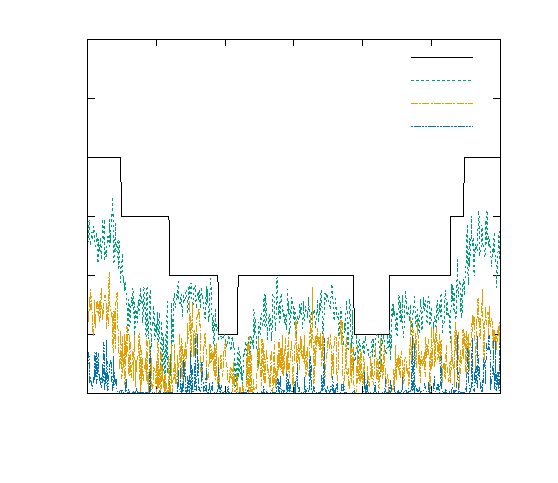
\includegraphics[width={253.00bp},height={217.00bp}]{armdisorder}}%
    \gplfronttext
  \end{picture}%
\endgroup

      \caption{رسانایی در مقابل انرژی برای نوارهای آرمچیر با عرض $18.59$\AA و با بی نظ‌‌می‌‌ توزیع شده در هر دو لبه در طول $758.81$\AA با اختلال نسبتا ضعیف $V_d=1\;eV$، \lr{BNR} های آرمچیر از فلز به نیمه‌هادی تبدیل ‌‌می‌‌شوند.}
      \label{armdisorder}
    \end{figure}
    
    \begin{figure*}[!ht]
      \centering
      % GNUPLOT: LaTeX picture with Postscript
\begingroup
  % Encoding inside the plot.  In the header of your document, this encoding
  % should to defined, e.g., by using
  % \usepackage[cp1252,<other encodings>]{inputenc}
  % \inputencoding{cp1252}%
  \makeatletter
  \providecommand\color[2][]{%
    \GenericError{(gnuplot) \space\space\space\@spaces}{%
      Package color not loaded in conjunction with
      terminal option `colourtext'%
    }{See the gnuplot documentation for explanation.%
    }{Either use 'blacktext' in gnuplot or load the package
      color.sty in LaTeX.}%
    \renewcommand\color[2][]{}%
  }%
  \providecommand\includegraphics[2][]{%
    \GenericError{(gnuplot) \space\space\space\@spaces}{%
      Package graphicx or graphics not loaded%
    }{See the gnuplot documentation for explanation.%
    }{The gnuplot epslatex terminal needs graphicx.sty or graphics.sty.}%
    \renewcommand\includegraphics[2][]{}%
  }%
  \providecommand\rotatebox[2]{#2}%
  \@ifundefined{ifGPcolor}{%
    \newif\ifGPcolor
    \GPcolorfalse
  }{}%
  \@ifundefined{ifGPblacktext}{%
    \newif\ifGPblacktext
    \GPblacktexttrue
  }{}%
  % define a \g@addto@macro without @ in the name:
  \let\gplgaddtomacro\g@addto@macro
  % define empty templates for all commands taking text:
  \gdef\gplbacktext{}%
  \gdef\gplfronttext{}%
  \makeatother
  \ifGPblacktext
    % no textcolor at all
    \def\colorrgb#1{}%
    \def\colorgray#1{}%
  \else
    % gray or color?
    \ifGPcolor
      \def\colorrgb#1{\color[rgb]{#1}}%
      \def\colorgray#1{\color[gray]{#1}}%
      \expandafter\def\csname LTw\endcsname{\color{white}}%
      \expandafter\def\csname LTb\endcsname{\color{black}}%
      \expandafter\def\csname LTa\endcsname{\color{black}}%
      \expandafter\def\csname LT0\endcsname{\color[rgb]{1,0,0}}%
      \expandafter\def\csname LT1\endcsname{\color[rgb]{0,1,0}}%
      \expandafter\def\csname LT2\endcsname{\color[rgb]{0,0,1}}%
      \expandafter\def\csname LT3\endcsname{\color[rgb]{1,0,1}}%
      \expandafter\def\csname LT4\endcsname{\color[rgb]{0,1,1}}%
      \expandafter\def\csname LT5\endcsname{\color[rgb]{1,1,0}}%
      \expandafter\def\csname LT6\endcsname{\color[rgb]{0,0,0}}%
      \expandafter\def\csname LT7\endcsname{\color[rgb]{1,0.3,0}}%
      \expandafter\def\csname LT8\endcsname{\color[rgb]{0.5,0.5,0.5}}%
    \else
      % gray
      \def\colorrgb#1{\color{black}}%
      \def\colorgray#1{\color[gray]{#1}}%
      \expandafter\def\csname LTw\endcsname{\color{white}}%
      \expandafter\def\csname LTb\endcsname{\color{black}}%
      \expandafter\def\csname LTa\endcsname{\color{black}}%
      \expandafter\def\csname LT0\endcsname{\color{black}}%
      \expandafter\def\csname LT1\endcsname{\color{black}}%
      \expandafter\def\csname LT2\endcsname{\color{black}}%
      \expandafter\def\csname LT3\endcsname{\color{black}}%
      \expandafter\def\csname LT4\endcsname{\color{black}}%
      \expandafter\def\csname LT5\endcsname{\color{black}}%
      \expandafter\def\csname LT6\endcsname{\color{black}}%
      \expandafter\def\csname LT7\endcsname{\color{black}}%
      \expandafter\def\csname LT8\endcsname{\color{black}}%
    \fi
  \fi
    \setlength{\unitlength}{0.0500bp}%
    \ifx\gptboxheight\undefined%
      \newlength{\gptboxheight}%
      \newlength{\gptboxwidth}%
      \newsavebox{\gptboxtext}%
    \fi%
    \setlength{\fboxrule}{0.5pt}%
    \setlength{\fboxsep}{1pt}%
\begin{picture}(7200.00,5040.00)%
    \gplgaddtomacro\gplbacktext{%
      \csname LTb\endcsname%%
      \put(814,704){\makebox(0,0)[r]{\strut{}$0$}}%
      \put(814,1161){\makebox(0,0)[r]{\strut{}$0.5$}}%
      \put(814,1618){\makebox(0,0)[r]{\strut{}$1$}}%
      \put(814,2076){\makebox(0,0)[r]{\strut{}$1.5$}}%
      \put(814,2533){\makebox(0,0)[r]{\strut{}$2$}}%
      \put(814,2990){\makebox(0,0)[r]{\strut{}$2.5$}}%
      \put(814,3447){\makebox(0,0)[r]{\strut{}$3$}}%
      \put(814,3905){\makebox(0,0)[r]{\strut{}$3.5$}}%
      \put(814,4362){\makebox(0,0)[r]{\strut{}$4$}}%
      \put(814,4819){\makebox(0,0)[r]{\strut{}$4.5$}}%
      \put(946,484){\makebox(0,0){\strut{}$0$}}%
      \put(1197,484){\makebox(0,0){\strut{}$2$}}%
      \put(1448,484){\makebox(0,0){\strut{}$4$}}%
      \put(1698,484){\makebox(0,0){\strut{}$6$}}%
      \put(1949,484){\makebox(0,0){\strut{}$8$}}%
      \put(2200,484){\makebox(0,0){\strut{}$10$}}%
      \put(2451,484){\makebox(0,0){\strut{}$12$}}%
      \put(2701,484){\makebox(0,0){\strut{}$14$}}%
      \put(2952,484){\makebox(0,0){\strut{}$16$}}%
      \put(3203,484){\makebox(0,0){\strut{}$18$}}%
      \put(1172,4613){\makebox(0,0)[l]{\strut{}(a)}}%
    }%
    \gplgaddtomacro\gplfronttext{%
      \csname LTb\endcsname%%
      \put(198,2761){\rotatebox{-270}{\makebox(0,0){\strut{}$G/G_0$}}}%
      \put(2074,154){\makebox(0,0){\strut{}Length(nm)$*10^{1}$}}%
      \csname LTb\endcsname%%
      \put(2216,4646){\makebox(0,0)[r]{\strut{}W=4}}%
      \csname LTb\endcsname%%
      \put(2216,4426){\makebox(0,0)[r]{\strut{}W=6}}%
      \csname LTb\endcsname%%
      \put(2216,4206){\makebox(0,0)[r]{\strut{}W=8}}%
    }%
    \gplgaddtomacro\gplbacktext{%
      \csname LTb\endcsname%%
      \put(4414,704){\makebox(0,0)[r]{\strut{}$0$}}%
      \put(4414,1078){\makebox(0,0)[r]{\strut{}$0.5$}}%
      \put(4414,1452){\makebox(0,0)[r]{\strut{}$1$}}%
      \put(4414,1826){\makebox(0,0)[r]{\strut{}$1.5$}}%
      \put(4414,2200){\makebox(0,0)[r]{\strut{}$2$}}%
      \put(4414,2574){\makebox(0,0)[r]{\strut{}$2.5$}}%
      \put(4414,2949){\makebox(0,0)[r]{\strut{}$3$}}%
      \put(4414,3323){\makebox(0,0)[r]{\strut{}$3.5$}}%
      \put(4414,3697){\makebox(0,0)[r]{\strut{}$4$}}%
      \put(4414,4071){\makebox(0,0)[r]{\strut{}$4.5$}}%
      \put(4414,4445){\makebox(0,0)[r]{\strut{}$5$}}%
      \put(4414,4819){\makebox(0,0)[r]{\strut{}$5.5$}}%
      \put(4546,484){\makebox(0,0){\strut{}$0$}}%
      \put(4997,484){\makebox(0,0){\strut{}$1$}}%
      \put(5449,484){\makebox(0,0){\strut{}$2$}}%
      \put(5900,484){\makebox(0,0){\strut{}$3$}}%
      \put(6352,484){\makebox(0,0){\strut{}$4$}}%
      \put(6803,484){\makebox(0,0){\strut{}$5$}}%
      \put(4772,4613){\makebox(0,0)[l]{\strut{}(b)}}%
    }%
    \gplgaddtomacro\gplfronttext{%
      \csname LTb\endcsname%%
      \put(3798,2761){\rotatebox{-270}{\makebox(0,0){\strut{}$G/G_0$}}}%
      \put(5674,154){\makebox(0,0){\strut{}$V_d(eV)$}}%
      \csname LTb\endcsname%%
      \put(5816,4646){\makebox(0,0)[r]{\strut{}W=4}}%
      \csname LTb\endcsname%%
      \put(5816,4426){\makebox(0,0)[r]{\strut{}W=6}}%
      \csname LTb\endcsname%%
      \put(5816,4206){\makebox(0,0)[r]{\strut{}W=8}}%
    }%
    \gplbacktext
    \put(0,0){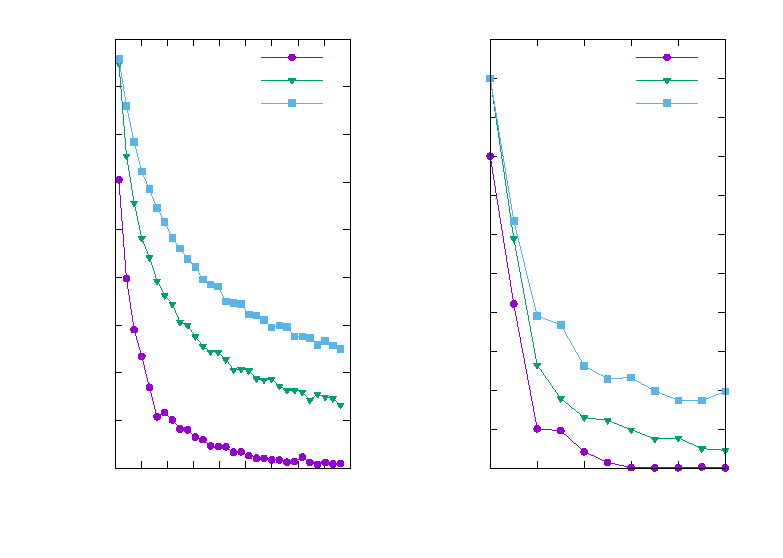
\includegraphics[width={361.00bp},height={253.00bp}]{zigzag-width-strangth}}%
    \gplfronttext
  \end{picture}%
\endgroup

      \caption{(الف) رسانایی در مقابل طول نوار با عرض‌های مختلف (از نظر تعداد سلول‌های واحد در یک ابرسلول) و قدرت بی نظ‌‌می‌‌ ثابت $V_d=2\;eV$. (ب) رسانایی در برابر استحکام بی نظ‌‌می‌‌ برای نوارهای زیگزاگ با بی نظ‌‌می‌‌ که در هر دو لبه به طول $876.68$\AA توزیع شده است.}
      \label{zigzag-width-strangth}
    \end{figure*}  

\begin{figure*}[!ht]
    \centering
    % GNUPLOT: LaTeX picture with Postscript
\begingroup
  % Encoding inside the plot.  In the header of your document, this encoding
  % should to defined, e.g., by using
  % \usepackage[cp1252,<other encodings>]{inputenc}
  % \inputencoding{cp1252}%
  \makeatletter
  \providecommand\color[2][]{%
    \GenericError{(gnuplot) \space\space\space\@spaces}{%
      Package color not loaded in conjunction with
      terminal option `colourtext'%
    }{See the gnuplot documentation for explanation.%
    }{Either use 'blacktext' in gnuplot or load the package
      color.sty in LaTeX.}%
    \renewcommand\color[2][]{}%
  }%
  \providecommand\includegraphics[2][]{%
    \GenericError{(gnuplot) \space\space\space\@spaces}{%
      Package graphicx or graphics not loaded%
    }{See the gnuplot documentation for explanation.%
    }{The gnuplot epslatex terminal needs graphicx.sty or graphics.sty.}%
    \renewcommand\includegraphics[2][]{}%
  }%
  \providecommand\rotatebox[2]{#2}%
  \@ifundefined{ifGPcolor}{%
    \newif\ifGPcolor
    \GPcolorfalse
  }{}%
  \@ifundefined{ifGPblacktext}{%
    \newif\ifGPblacktext
    \GPblacktexttrue
  }{}%
  % define a \g@addto@macro without @ in the name:
  \let\gplgaddtomacro\g@addto@macro
  % define empty templates for all commands taking text:
  \gdef\gplbacktext{}%
  \gdef\gplfronttext{}%
  \makeatother
  \ifGPblacktext
    % no textcolor at all
    \def\colorrgb#1{}%
    \def\colorgray#1{}%
  \else
    % gray or color?
    \ifGPcolor
      \def\colorrgb#1{\color[rgb]{#1}}%
      \def\colorgray#1{\color[gray]{#1}}%
      \expandafter\def\csname LTw\endcsname{\color{white}}%
      \expandafter\def\csname LTb\endcsname{\color{black}}%
      \expandafter\def\csname LTa\endcsname{\color{black}}%
      \expandafter\def\csname LT0\endcsname{\color[rgb]{1,0,0}}%
      \expandafter\def\csname LT1\endcsname{\color[rgb]{0,1,0}}%
      \expandafter\def\csname LT2\endcsname{\color[rgb]{0,0,1}}%
      \expandafter\def\csname LT3\endcsname{\color[rgb]{1,0,1}}%
      \expandafter\def\csname LT4\endcsname{\color[rgb]{0,1,1}}%
      \expandafter\def\csname LT5\endcsname{\color[rgb]{1,1,0}}%
      \expandafter\def\csname LT6\endcsname{\color[rgb]{0,0,0}}%
      \expandafter\def\csname LT7\endcsname{\color[rgb]{1,0.3,0}}%
      \expandafter\def\csname LT8\endcsname{\color[rgb]{0.5,0.5,0.5}}%
    \else
      % gray
      \def\colorrgb#1{\color{black}}%
      \def\colorgray#1{\color[gray]{#1}}%
      \expandafter\def\csname LTw\endcsname{\color{white}}%
      \expandafter\def\csname LTb\endcsname{\color{black}}%
      \expandafter\def\csname LTa\endcsname{\color{black}}%
      \expandafter\def\csname LT0\endcsname{\color{black}}%
      \expandafter\def\csname LT1\endcsname{\color{black}}%
      \expandafter\def\csname LT2\endcsname{\color{black}}%
      \expandafter\def\csname LT3\endcsname{\color{black}}%
      \expandafter\def\csname LT4\endcsname{\color{black}}%
      \expandafter\def\csname LT5\endcsname{\color{black}}%
      \expandafter\def\csname LT6\endcsname{\color{black}}%
      \expandafter\def\csname LT7\endcsname{\color{black}}%
      \expandafter\def\csname LT8\endcsname{\color{black}}%
    \fi
  \fi
    \setlength{\unitlength}{0.0500bp}%
    \ifx\gptboxheight\undefined%
      \newlength{\gptboxheight}%
      \newlength{\gptboxwidth}%
      \newsavebox{\gptboxtext}%
    \fi%
    \setlength{\fboxrule}{0.5pt}%
    \setlength{\fboxsep}{1pt}%
\begin{picture}(7200.00,5040.00)%
    \gplgaddtomacro\gplbacktext{%
      \csname LTb\endcsname%%
      \put(814,704){\makebox(0,0)[r]{\strut{}$0$}}%
      \put(814,1390){\makebox(0,0)[r]{\strut{}$0.5$}}%
      \put(814,2076){\makebox(0,0)[r]{\strut{}$1$}}%
      \put(814,2762){\makebox(0,0)[r]{\strut{}$1.5$}}%
      \put(814,3447){\makebox(0,0)[r]{\strut{}$2$}}%
      \put(814,4133){\makebox(0,0)[r]{\strut{}$2.5$}}%
      \put(814,4819){\makebox(0,0)[r]{\strut{}$3$}}%
      \put(946,484){\makebox(0,0){\strut{}$0$}}%
      \put(1322,484){\makebox(0,0){\strut{}$5$}}%
      \put(1698,484){\makebox(0,0){\strut{}$10$}}%
      \put(2075,484){\makebox(0,0){\strut{}$15$}}%
      \put(2451,484){\makebox(0,0){\strut{}$20$}}%
      \put(2827,484){\makebox(0,0){\strut{}$25$}}%
      \put(3203,484){\makebox(0,0){\strut{}$30$}}%
      \put(1172,4613){\makebox(0,0)[l]{\strut{}(a)}}%
    }%
    \gplgaddtomacro\gplfronttext{%
      \csname LTb\endcsname%%
      \put(209,2761){\rotatebox{-270}{\makebox(0,0){\strut{}$G/G_0$}}}%
      \put(2074,154){\makebox(0,0){\strut{}Lenght(nm)$*10^{1}$}}%
      \csname LTb\endcsname%%
      \put(2216,4646){\makebox(0,0)[r]{\strut{}W=4}}%
      \csname LTb\endcsname%%
      \put(2216,4426){\makebox(0,0)[r]{\strut{}W=6}}%
      \csname LTb\endcsname%%
      \put(2216,4206){\makebox(0,0)[r]{\strut{}W=8}}%
    }%
    \gplgaddtomacro\gplbacktext{%
      \csname LTb\endcsname%%
      \put(4414,704){\makebox(0,0)[r]{\strut{}$0$}}%
      \put(4414,1390){\makebox(0,0)[r]{\strut{}$0.5$}}%
      \put(4414,2076){\makebox(0,0)[r]{\strut{}$1$}}%
      \put(4414,2762){\makebox(0,0)[r]{\strut{}$1.5$}}%
      \put(4414,3447){\makebox(0,0)[r]{\strut{}$2$}}%
      \put(4414,4133){\makebox(0,0)[r]{\strut{}$2.5$}}%
      \put(4414,4819){\makebox(0,0)[r]{\strut{}$3$}}%
      \put(4546,484){\makebox(0,0){\strut{}$0$}}%
      \put(4922,484){\makebox(0,0){\strut{}$0.5$}}%
      \put(5298,484){\makebox(0,0){\strut{}$1$}}%
      \put(5675,484){\makebox(0,0){\strut{}$1.5$}}%
      \put(6051,484){\makebox(0,0){\strut{}$2$}}%
      \put(6427,484){\makebox(0,0){\strut{}$2.5$}}%
      \put(6803,484){\makebox(0,0){\strut{}$3$}}%
      \put(4772,4613){\makebox(0,0)[l]{\strut{}(b)}}%
    }%
    \gplgaddtomacro\gplfronttext{%
      \csname LTb\endcsname%%
      \put(3809,2761){\rotatebox{-270}{\makebox(0,0){\strut{}$G/G_0$}}}%
      \put(5674,154){\makebox(0,0){\strut{}$V_d(eV)$}}%
      \csname LTb\endcsname%%
      \put(5816,4646){\makebox(0,0)[r]{\strut{}W=4}}%
      \csname LTb\endcsname%%
      \put(5816,4426){\makebox(0,0)[r]{\strut{}W=6}}%
      \csname LTb\endcsname%%
      \put(5816,4206){\makebox(0,0)[r]{\strut{}W=8}}%
    }%
    \gplbacktext
    \put(0,0){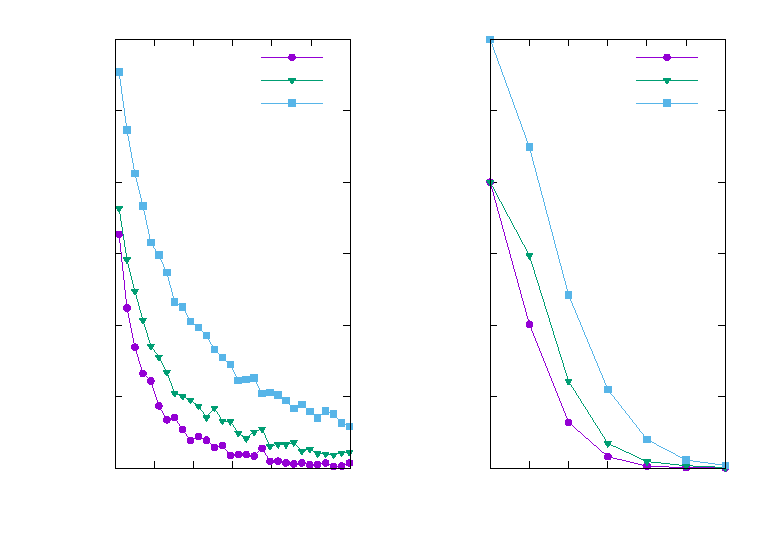
\includegraphics[width={360.00bp},height={252.00bp}]{armchair-width-strangth}}%
    \gplfronttext
  \end{picture}%
\endgroup

    \caption{(الف) رسانایی در مقابل طول روبان آرمچیر با عرض‌های مختلف (از نظر تعداد سلول‌های واحد در یک سوپرسل) و قدرت بی نظ‌‌می‌‌ ثابت $V_d=1\;eV$. (ب) رسانایی در مقابل استحکام بی نظ‌‌می‌‌ برای روبان‌های آرمچیر با بی نظ‌‌می‌‌ که در هر دو لبه به طول \lr{\AA}$758.81$ توزیع شده است.}
    \label{armchair-width-strangth}
  \end{figure*}

\subsection{اختلال ضعیف جایگزیده سازی اندرسون در نانونوارهای بورفین:}
پدیده‌ای است که ناشی از تداخل امواج منتشر شده از مسیرهای متعدد است که در انواع سیستم‌های موجی قابل مشاهده است \cite{Strybulevych2008,Chabe2008,Ying2016,Manai2015}. درک کامل جایگزیده‌سازی اندرسون امکانپذیر نخواهد بود مگر اینکه عواملی را کنترل کنیم که بر آن تأثیر ‌می‌گذارند، از جمله برهمکنش‌های بین ذرهای، بعد، تقارن معکوس زمانی، و ماهیت ‌میکروسکوپی اختلال. یکی از مناسب‌ترین و قابل کنترل‌ترین نمونه‌های این امر ‌می‌تواند سیستم‌های کوانتو‌‌می اتم‌های فوق سرد باشد که منجر به درک عمیق جایگزیده‌سازی اندرسون ‌می‌شود \cite{Georgescu2014}. جایگزیدگی اندرسون در فیزیک حالت جامد بسیار جالب است زیرا پیش بینی ‌‌می‌‌کند که یک الکترون ممکن است در یک شبکه بی نظم بی حرکت شود \cite{Georgescu2014}. از قضیه بلوخ، ‌می‌‌دانیم که در یک سیستم مکانیکی کوانتو‌‌می‌‌ با یک همیلتونی تناوبی فضایی، ویژه حالت‌های تک ذره‌ای در سراسر فضا گسترش یافته‌اند. وجود اختلال ایستا تقارن انتقالی کریستالی و‌ها‌میلتونی را ‌‌می‌‌شکند و در نتیجه احتمال ویژه حالت‌های را افزایش ‌‌می‌‌دهد که به صورت تصاعدی موضعی ‌‌می‌‌شوند. به طور کلی، هر چه ‌میزان اختلال بیشتر باشد، تعداد ویژه حالت‌های موضعی بیشتر  ‌می‌شود و در برخی موارد، زمانی که اختلال به اندازه کافی بزرگ است، همه حالت‌های گسترش یافته را به حالت‌های موضعی تبدیل ‌می‌کند و باعث ترابرد اندرسون ‌می‌‌شود. ویژه حالت‌های گسترده یا موضعی مربوط به حضور یا عدم وجود ذرات برای ترابرد در مقیاس طول ماکروسکوپی است. (حالت‌های گسترش یافته منجر به جابجایی مربع ‌میانگین ‌می‌شود که با گذشت زمان برای مدت طولانی رشد ‌می‌کند، در حالی که حالت‌های موضعی رشد ‌می‌‌کنند.) بنابراین، جایگزیده سازی اندرسون ‌می‌‌تواند پدیده‌های ترابرد، از جمله ترابرد عایق فلزی در نیمرساناها را توضیح دهد.

در اینجا، از آنجایی که با یک سیستم شبه یک بعدی سروکار داریم، ناخالصی‌ها تنها در لبه‌های بالایی و پایینی نانوروبان‌ها با اختصاص یک متغیر تصادفی نامرتبط به هر یک از آنها توزیع ‌‌می‌‌شوند. ناخالصی‌ها در امتداد لبه‌های نانوروبان توزیع ‌‌می‌‌شوند و قدرت بالقوه آنها به طور تصادفی از محدوده $[-V_d, V_d]$ انتخاب ‌‌می‌‌شود. همانطور که در شکل\ref{zigzagdisorder} مشاهده ‌‌می‌‌شود، اگرچه پتانسیل‌های بسیار ضعیف رسانایی را کاهش ‌‌می‌‌دهند، اما نمی‌‌توانند باعث جایگزیده سازی اندرسون شوند. همانطور که قدرت پتانسیل افزایش ‌‌می‌‌یابد، واضح است که جایگزیده سازی در انرژی‌هایی در حدود $-0.5\;eV$ زمانی که $V_d = 2\;eV$ رخ ‌‌می‌‌دهد. به عبارت دیگر، برای قدرت پتانسیل بسیار ضعیف، طول جایگزیده سازی بسیار طولانی است. این را ‌‌می‌‌توان با این واقعیت توضیح داد که در یک سیستم یک بعدی بی نهایت، حتی یک اختلال بسیار ضعیف ‌‌می‌‌تواند تداخل سازنده را مختل کند و باعث رسانایی صفر شود. طول جایگزیده‌سازی به عنوان طولی تعریف ‌می‌شود که در آن همه ویژه حالت‌های بلوخ به صورت فضایی گسترش یافته به حالت‌های موضعی تغییر ‌می‌کنند و در نتیجه رسانایی صفر ‌می‌شود. همانطور که انتظار ‌‌می‌‌رود، با افزایش طول نوار با قدرت پتانسیل $2 \;eV$ در لبه‌ها، رسانایی احتمالاً به طور تصاعدی کاهش ‌می‌‌یابد. شکل\ref{zigzag-width-strangth}(الف) یک رسانایی در انرژی فر‌‌می‌‌ را با ‌میانگین بیش از 1000 پیکربندی مختلف از انتخاب‌های تصادفی پتانسیل در لبه‌ها برای عرض‌های مختلف \gls{ZBNR} نشان ‌‌می‌‌دهد، که نشان دهنده کاهش نمایی در رسانایی است. در \gls{ZBNR}ها، تعداد کانالهای رسانایی در اطراف انرژی فر‌‌می‌‌ به عرض نانوروبانها بستگی دارد، که تفاوت بین رسانایی نانوروبان‌ها‌یی با طول‌های کوچک با عرض‌های مختلف را در تضاد واضح با مورد گرافین توضیح ‌می‌دهد. علاوه بر این، طول طول جایگزیده سازی اندرسون در \gls{ZBNR}ها (تقریباً 180-1800 نانومتر برای عرض سلول‌های 4-8 واحد) بسیار بیشتر از \lr{ZGNR}ها است (تقریباً 200-800 آنگستروم که با آنچه توسط \gls{Li} و همکاران گزارش شده مطابقت دارد).\cite{Lee1985} در گرافین). همانطور که مشاهده ‌‌می‌‌شود، هر چه قدرت اختلال بیشتر باشد، طول جایگزیده سازی کوتاه‌تر به دست ‌‌می‌‌آید. رسانایی \gls{ABNR}ها با عرض \lr{\AA} 10.24 و طول نانوروبان \lr{\AA} 758.81 در شکل\ref{armdisorder} نشان داده شده است. برخلاف \gls{ZBNR}ها، حتی قدرت بی نظ‌‌می‌‌ بسیار ضعیف نیز ممکن است اثرات قابل توجهی بر رسانایی داشته باشد، با طول جایگزیده سازی بسیار کوتاه تر از طول جایگزیده سازی مشاهده شده در \gls{ZBNR}ها شکل\ref{armchair-width-strangth}، تغییر رسانایی در \gls{ABNR}ها را به عنوان تابعی از طول شکل\ref{armchair-width-strangth}(الف) و قدرت بالقوه شکل\ref{armchair-width-strangth}(ب) در انرژی انرژی فر‌می‌، که از طریق ‌میانگین بیش از 1000 پیکربندی مختلف اختلال لبه محاسبه شده است، نشان ‌‌می‌‌دهد. هر دو شکل نشان دهنده کاهش نمایی رسانایی زمانی است که طول (یا قدرت پتانسیل) در \gls{ABNR}‌ هاافزایش ‌‌می‌‌یابد. همانطور که انتظار ‌‌می‌‌رود، افزایش در تعداد کانال‌های رسانایی زمانی مشاهده ‌‌می‌‌شود که عرض \gls{ABNR}‌ ها افزایش ‌‌می‌‌یابد، که از نظر کیفی مشابه آنچه برای \gls{ZBNR} به دست آمده است. دلیل فیزیکی پشت تاثیر بیشتر اختلال ضعیف بر هدایت \gls{ABNR}ها در مقایسه با \gls{ZBNR}‌ها را ‌‌می‌‌توان با سرعت بالاتر سرعت گروه الکترونی در \gls{ZBNR}‌ها در مقایسه با \gls{ABNR}‌ها در محدوده انرژی فر‌‌می‌‌ درک کرد.

\begin{figure*}
  \centering
  \includegraphics[width=0.8\linewidth]{./figures/Shematic3.png}
\caption{به صورت شماتیک ساختار یک دریچه اسپینی مبتنی بر $\beta$-بوروفین را با الکترودهای مغناطیسی نشان ‌‌می‌‌دهد، که در آن بردارهای مغناطیسی دو الکترود ‌‌می‌‌توانند زاویه نسبی $\theta$ داشته باشند. مغناطیسی شدن الکترودها ناشی از زیرلایه مغناطیسی است که روی آن قرار ‌‌می‌‌گیرند که ‌‌می‌‌توان آن را به صورت تجربی کنترل کرد. در قسمت بالای شکل، ‌بورفین نانوروبان با لبه‌های آرمچیر و در قسمت پایین شکل، نانوروبان ‌بورفین زیگزاگ به تصویر کشیده شده است. سلول واحد ‌بورفین با اتم‌های بور که در یک بورفین لبه زیگزاگ برچسب‌گذاری شده‌اند در جدول \ref{tbl:hoppingtable} نشان داده شده است، جایی که انرژی‌های موجود در محل و پارامترهای جهش اتم‌ها آورده شده است.}
  \label{fig:model}
\end{figure*}
    
\begin{figure*}[!ht]
  \begin{latin}
  \centering
  \resizebox{0.45\textwidth}{!}{\input{./figures/Armchair-Antiparallel-conductance-revise.tex}}
  \resizebox{0.45\textwidth}{!}{% GNUPLOT: LaTeX picture with Postscript
\begin{latin}
\begingroup
  % Encoding inside the plot.  In the header of your document, this encoding
  % should to defined, e.g., by using
  % \usepackage[cp1252,<other encodings>]{inputenc}
  % \inputencoding{cp1252}%
  \makeatletter
  \providecommand\color[2][]{%
    \GenericError{(gnuplot) \space\space\space\@spaces}{%
      Package color not loaded in conjunction with
      terminal option `colourtext'%
    }{See the gnuplot documentation for explanation.%
    }{Either use 'blacktext' in gnuplot or load the package
      color.sty in LaTeX.}%
    \renewcommand\color[2][]{}%
  }%
  \providecommand\includegraphics[2][]{%
    \GenericError{(gnuplot) \space\space\space\@spaces}{%
      Package graphicx or graphics not loaded%
    }{See the gnuplot documentation for explanation.%
    }{The gnuplot epslatex terminal needs graphicx.sty or graphics.sty.}%
    \renewcommand\includegraphics[2][]{}%
  }%
  \providecommand\rotatebox[2]{#2}%
  \@ifundefined{ifGPcolor}{%
    \newif\ifGPcolor
    \GPcolorfalse
  }{}%
  \@ifundefined{ifGPblacktext}{%
    \newif\ifGPblacktext
    \GPblacktexttrue
  }{}%
  % define a \g@addto@macro without @ in the name:
  \let\gplgaddtomacro\g@addto@macro
  % define empty templates for all commands taking text:
  \gdef\gplbacktext{}%
  \gdef\gplfronttext{}%
  \makeatother
  \ifGPblacktext
    % no textcolor at all
    \def\colorrgb#1{}%
    \def\colorgray#1{}%
  \else
    % gray or color?
    \ifGPcolor
      \def\colorrgb#1{\color[rgb]{#1}}%
      \def\colorgray#1{\color[gray]{#1}}%
      \expandafter\def\csname LTw\endcsname{\color{white}}%
      \expandafter\def\csname LTb\endcsname{\color{black}}%
      \expandafter\def\csname LTa\endcsname{\color{black}}%
      \expandafter\def\csname LT0\endcsname{\color[rgb]{1,0,0}}%
      \expandafter\def\csname LT1\endcsname{\color[rgb]{0,1,0}}%
      \expandafter\def\csname LT2\endcsname{\color[rgb]{0,0,1}}%
      \expandafter\def\csname LT3\endcsname{\color[rgb]{1,0,1}}%
      \expandafter\def\csname LT4\endcsname{\color[rgb]{0,1,1}}%
      \expandafter\def\csname LT5\endcsname{\color[rgb]{1,1,0}}%
      \expandafter\def\csname LT6\endcsname{\color[rgb]{0,0,0}}%
      \expandafter\def\csname LT7\endcsname{\color[rgb]{1,0.3,0}}%
      \expandafter\def\csname LT8\endcsname{\color[rgb]{0.5,0.5,0.5}}%
    \else
      % gray
      \def\colorrgb#1{\color{black}}%
      \def\colorgray#1{\color[gray]{#1}}%
      \expandafter\def\csname LTw\endcsname{\color{white}}%
      \expandafter\def\csname LTb\endcsname{\color{black}}%
      \expandafter\def\csname LTa\endcsname{\color{black}}%
      \expandafter\def\csname LT0\endcsname{\color{black}}%
      \expandafter\def\csname LT1\endcsname{\color{black}}%
      \expandafter\def\csname LT2\endcsname{\color{black}}%
      \expandafter\def\csname LT3\endcsname{\color{black}}%
      \expandafter\def\csname LT4\endcsname{\color{black}}%
      \expandafter\def\csname LT5\endcsname{\color{black}}%
      \expandafter\def\csname LT6\endcsname{\color{black}}%
      \expandafter\def\csname LT7\endcsname{\color{black}}%
      \expandafter\def\csname LT8\endcsname{\color{black}}%
    \fi
  \fi
    \setlength{\unitlength}{0.0500bp}%
    \ifx\gptboxheight\undefined%
      \newlength{\gptboxheight}%
      \newlength{\gptboxwidth}%
      \newsavebox{\gptboxtext}%
    \fi%
    \setlength{\fboxrule}{0.5pt}%
    \setlength{\fboxsep}{1pt}%
\begin{picture}(7200.00,5040.00)%
    \gplgaddtomacro\gplbacktext{%
      \csname LTb\endcsname%%
      \put(900,4200){\makebox(0,0)[r]{\strut{}$B$}}%
      \put(550,704){\makebox(0,0)[r]{\strut{}$0$}}%
      \put(550,1112){\makebox(0,0)[r]{\strut{}$1$}}%
      \put(550,1521){\makebox(0,0)[r]{\strut{}$2$}}%
      \put(550,1929){\makebox(0,0)[r]{\strut{}$3$}}%
      \put(550,2337){\makebox(0,0)[r]{\strut{}$4$}}%
      \put(550,2746){\makebox(0,0)[r]{\strut{}$5$}}%
      \put(550,3154){\makebox(0,0)[r]{\strut{}$6$}}%
      \put(550,3562){\makebox(0,0)[r]{\strut{}$7$}}%
      \put(550,3971){\makebox(0,0)[r]{\strut{}$8$}}%
      \put(550,4379){\makebox(0,0)[r]{\strut{}$9$}}%
      \put(682,484){\makebox(0,0){\strut{}$-4$}}%
      \put(1447,484){\makebox(0,0){\strut{}$-3$}}%
      \put(2212,484){\makebox(0,0){\strut{}$-2$}}%
      \put(2977,484){\makebox(0,0){\strut{}$-1$}}%
      \put(3743,484){\makebox(0,0){\strut{}$0$}}%
      \put(4508,484){\makebox(0,0){\strut{}$1$}}%
      \put(5273,484){\makebox(0,0){\strut{}$2$}}%
      \put(6038,484){\makebox(0,0){\strut{}$3$}}%
      \put(6803,484){\makebox(0,0){\strut{}$4$}}%
    }%
    \gplgaddtomacro\gplfronttext{%
      \csname LTb\endcsname%%
      \put(209,2541){\rotatebox{-270}{\makebox(0,0){\strut{}$G(e^2/h)$}}}%
      \put(3742,154){\makebox(0,0){\strut{}$E(eV)$}}%
      \csname LTb\endcsname%%
      \put(2522,4206){\makebox(0,0)[r]{\strut{}$M=0$}}%
      \csname LTb\endcsname%%
      \put(2522,3986){\makebox(0,0)[r]{\strut{}$M=0.05$}}%
      \csname LTb\endcsname%%
      \put(4169,4206){\makebox(0,0)[r]{\strut{}$M=0.1$}}%
      \csname LTb\endcsname%%
      \put(4169,3986){\makebox(0,0)[r]{\strut{}$M=0.2$}}%
      \csname LTb\endcsname%%
      \put(5816,4206){\makebox(0,0)[r]{\strut{}$M=0.3$}}%
      \csname LTb\endcsname%%
      \put(3742,4709){\makebox(0,0){\strut{}Parallel}}%
    }%
    \gplbacktext
    \put(0,0){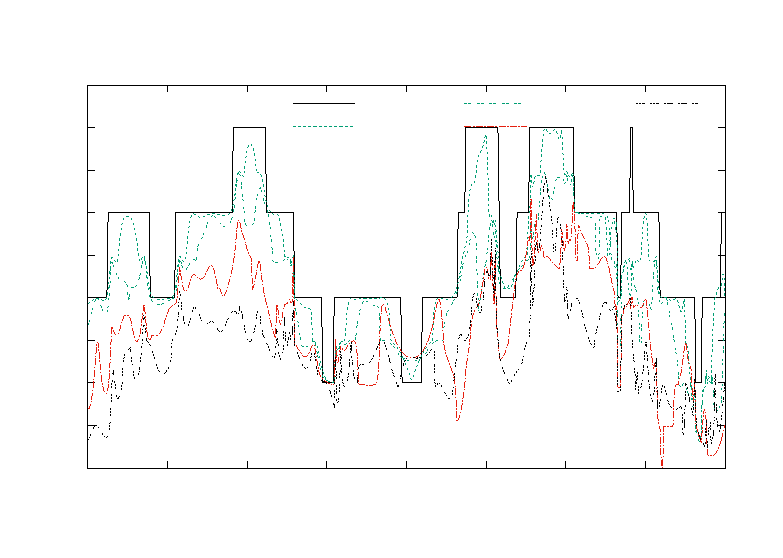
\includegraphics[width={360.00bp},height={252.00bp}]{armchair-parallel-conductance-revise}}%
    \gplfronttext
  \end{picture}%
\endgroup
\end{latin}}
  \resizebox{0.45\textwidth}{!}{% GNUPLOT: LaTeX picture with Postscript
\begingroup
  % Encoding inside the plot.  In the header of your document, this encoding
  % should to defined, e.g., by using
  % \usepackage[cp1252,<other encodings>]{inputenc}
  % \inputencoding{cp1252}%
  \makeatletter
  \providecommand\color[2][]{%
    \GenericError{(gnuplot) \space\space\space\@spaces}{%
      Package color not loaded in conjunction with
      terminal option `colourtext'%
    }{See the gnuplot documentation for explanation.%
    }{Either use 'blacktext' in gnuplot or load the package
      color.sty in LaTeX.}%
    \renewcommand\color[2][]{}%
  }%
  \providecommand\includegraphics[2][]{%
    \GenericError{(gnuplot) \space\space\space\@spaces}{%
      Package graphicx or graphics not loaded%
    }{See the gnuplot documentation for explanation.%
    }{The gnuplot epslatex terminal needs graphicx.sty or graphics.sty.}%
    \renewcommand\includegraphics[2][]{}%
  }%
  \providecommand\rotatebox[2]{#2}%
  \@ifundefined{ifGPcolor}{%
    \newif\ifGPcolor
    \GPcolorfalse
  }{}%
  \@ifundefined{ifGPblacktext}{%
    \newif\ifGPblacktext
    \GPblacktexttrue
  }{}%
  % define a \g@addto@macro without @ in the name:
  \let\gplgaddtomacro\g@addto@macro
  % define empty templates for all commands taking text:
  \gdef\gplbacktext{}%
  \gdef\gplfronttext{}%
  \makeatother
  \ifGPblacktext
    % no textcolor at all
    \def\colorrgb#1{}%
    \def\colorgray#1{}%
  \else
    % gray or color?
    \ifGPcolor
      \def\colorrgb#1{\color[rgb]{#1}}%
      \def\colorgray#1{\color[gray]{#1}}%
      \expandafter\def\csname LTw\endcsname{\color{white}}%
      \expandafter\def\csname LTb\endcsname{\color{black}}%
      \expandafter\def\csname LTa\endcsname{\color{black}}%
      \expandafter\def\csname LT0\endcsname{\color[rgb]{1,0,0}}%
      \expandafter\def\csname LT1\endcsname{\color[rgb]{0,1,0}}%
      \expandafter\def\csname LT2\endcsname{\color[rgb]{0,0,1}}%
      \expandafter\def\csname LT3\endcsname{\color[rgb]{1,0,1}}%
      \expandafter\def\csname LT4\endcsname{\color[rgb]{0,1,1}}%
      \expandafter\def\csname LT5\endcsname{\color[rgb]{1,1,0}}%
      \expandafter\def\csname LT6\endcsname{\color[rgb]{0,0,0}}%
      \expandafter\def\csname LT7\endcsname{\color[rgb]{1,0.3,0}}%
      \expandafter\def\csname LT8\endcsname{\color[rgb]{0.5,0.5,0.5}}%
    \else
      % gray
      \def\colorrgb#1{\color{black}}%
      \def\colorgray#1{\color[gray]{#1}}%
      \expandafter\def\csname LTw\endcsname{\color{white}}%
      \expandafter\def\csname LTb\endcsname{\color{black}}%
      \expandafter\def\csname LTa\endcsname{\color{black}}%
      \expandafter\def\csname LT0\endcsname{\color{black}}%
      \expandafter\def\csname LT1\endcsname{\color{black}}%
      \expandafter\def\csname LT2\endcsname{\color{black}}%
      \expandafter\def\csname LT3\endcsname{\color{black}}%
      \expandafter\def\csname LT4\endcsname{\color{black}}%
      \expandafter\def\csname LT5\endcsname{\color{black}}%
      \expandafter\def\csname LT6\endcsname{\color{black}}%
      \expandafter\def\csname LT7\endcsname{\color{black}}%
      \expandafter\def\csname LT8\endcsname{\color{black}}%
    \fi
  \fi
    \setlength{\unitlength}{0.0500bp}%
    \ifx\gptboxheight\undefined%
      \newlength{\gptboxheight}%
      \newlength{\gptboxwidth}%
      \newsavebox{\gptboxtext}%
    \fi%
    \setlength{\fboxrule}{0.5pt}%
    \setlength{\fboxsep}{1pt}%
\begin{picture}(7200.00,5040.00)%
    \gplgaddtomacro\gplbacktext{%
      \csname LTb\endcsname%%
      \put(1000,4200){\makebox(0,0)[r]{\strut{}$C$}}%
      \put(682,704){\makebox(0,0)[r]{\strut{}$2$}}%
      \put(682,1163){\makebox(0,0)[r]{\strut{}$4$}}%
      \put(682,1623){\makebox(0,0)[r]{\strut{}$6$}}%
      \put(682,2082){\makebox(0,0)[r]{\strut{}$8$}}%
      \put(682,2542){\makebox(0,0)[r]{\strut{}$10$}}%
      \put(682,3001){\makebox(0,0)[r]{\strut{}$12$}}%
      \put(682,3460){\makebox(0,0)[r]{\strut{}$14$}}%
      \put(682,3920){\makebox(0,0)[r]{\strut{}$16$}}%
      \put(682,4379){\makebox(0,0)[r]{\strut{}$18$}}%
      \put(814,484){\makebox(0,0){\strut{}$-4$}}%
      \put(1563,484){\makebox(0,0){\strut{}$-3$}}%
      \put(2311,484){\makebox(0,0){\strut{}$-2$}}%
      \put(3060,484){\makebox(0,0){\strut{}$-1$}}%
      \put(3809,484){\makebox(0,0){\strut{}$0$}}%
      \put(4557,484){\makebox(0,0){\strut{}$1$}}%
      \put(5306,484){\makebox(0,0){\strut{}$2$}}%
      \put(6054,484){\makebox(0,0){\strut{}$3$}}%
      \put(6803,484){\makebox(0,0){\strut{}$4$}}%
    }%
    \gplgaddtomacro\gplfronttext{%
      \csname LTb\endcsname%%
      \put(209,2541){\rotatebox{-270}{\makebox(0,0){\strut{}$G(e^2/h)$}}}%
      \put(3808,154){\makebox(0,0){\strut{}$E(eV)$}}%
      \csname LTb\endcsname%%
      \put(2522,4206){\makebox(0,0)[r]{\strut{}$M=0$}}%
      \csname LTb\endcsname%%
      \put(2522,3986){\makebox(0,0)[r]{\strut{}$M=0.05$}}%
      \csname LTb\endcsname%%
      \put(4169,4206){\makebox(0,0)[r]{\strut{}$M=0.1$}}%
      \csname LTb\endcsname%%
      \put(4169,3986){\makebox(0,0)[r]{\strut{}$M=0.2$}}%
      \csname LTb\endcsname%%
      \put(5816,4206){\makebox(0,0)[r]{\strut{}$M=0.3$}}%
      \csname LTb\endcsname%%
      \put(3808,4709){\makebox(0,0){\strut{}AntiParallel}}%
    }%
    \gplbacktext
    \put(0,0){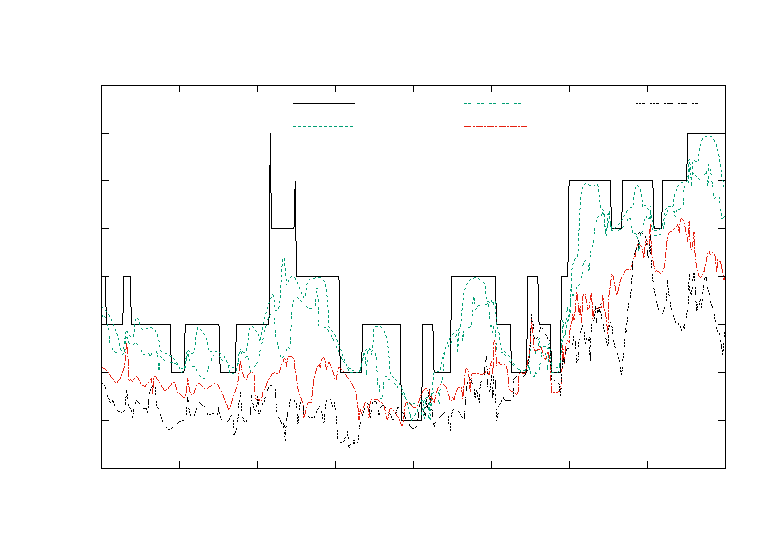
\includegraphics[width={360.00bp},height={252.00bp}]{zigzag-antiparallel-conductance-revise}}%
    \gplfronttext
  \end{picture}%
\endgroup
}
  \resizebox{0.45\textwidth}{!}{% GNUPLOT: LaTeX picture with Postscript
\begingroup
  % Encoding inside the plot.  In the header of your document, this encoding
  % should to defined, e.g., by using
  % \usepackage[cp1252,<other encodings>]{inputenc}
  % \inputencoding{cp1252}%
  \makeatletter
  \providecommand\color[2][]{%
    \GenericError{(gnuplot) \space\space\space\@spaces}{%
      Package color not loaded in conjunction with
      terminal option `colourtext'%
    }{See the gnuplot documentation for explanation.%
    }{Either use 'blacktext' in gnuplot or load the package
      color.sty in LaTeX.}%
    \renewcommand\color[2][]{}%
  }%
  \providecommand\includegraphics[2][]{%
    \GenericError{(gnuplot) \space\space\space\@spaces}{%
      Package graphicx or graphics not loaded%
    }{See the gnuplot documentation for explanation.%
    }{The gnuplot epslatex terminal needs graphicx.sty or graphics.sty.}%
    \renewcommand\includegraphics[2][]{}%
  }%
  \providecommand\rotatebox[2]{#2}%
  \@ifundefined{ifGPcolor}{%
    \newif\ifGPcolor
    \GPcolorfalse
  }{}%
  \@ifundefined{ifGPblacktext}{%
    \newif\ifGPblacktext
    \GPblacktexttrue
  }{}%
  % define a \g@addto@macro without @ in the name:
  \let\gplgaddtomacro\g@addto@macro
  % define empty templates for all commands taking text:
  \gdef\gplbacktext{}%
  \gdef\gplfronttext{}%
  \makeatother
  \ifGPblacktext
    % no textcolor at all
    \def\colorrgb#1{}%
    \def\colorgray#1{}%
  \else
    % gray or color?
    \ifGPcolor
      \def\colorrgb#1{\color[rgb]{#1}}%
      \def\colorgray#1{\color[gray]{#1}}%
      \expandafter\def\csname LTw\endcsname{\color{white}}%
      \expandafter\def\csname LTb\endcsname{\color{black}}%
      \expandafter\def\csname LTa\endcsname{\color{black}}%
      \expandafter\def\csname LT0\endcsname{\color[rgb]{1,0,0}}%
      \expandafter\def\csname LT1\endcsname{\color[rgb]{0,1,0}}%
      \expandafter\def\csname LT2\endcsname{\color[rgb]{0,0,1}}%
      \expandafter\def\csname LT3\endcsname{\color[rgb]{1,0,1}}%
      \expandafter\def\csname LT4\endcsname{\color[rgb]{0,1,1}}%
      \expandafter\def\csname LT5\endcsname{\color[rgb]{1,1,0}}%
      \expandafter\def\csname LT6\endcsname{\color[rgb]{0,0,0}}%
      \expandafter\def\csname LT7\endcsname{\color[rgb]{1,0.3,0}}%
      \expandafter\def\csname LT8\endcsname{\color[rgb]{0.5,0.5,0.5}}%
    \else
      % gray
      \def\colorrgb#1{\color{black}}%
      \def\colorgray#1{\color[gray]{#1}}%
      \expandafter\def\csname LTw\endcsname{\color{white}}%
      \expandafter\def\csname LTb\endcsname{\color{black}}%
      \expandafter\def\csname LTa\endcsname{\color{black}}%
      \expandafter\def\csname LT0\endcsname{\color{black}}%
      \expandafter\def\csname LT1\endcsname{\color{black}}%
      \expandafter\def\csname LT2\endcsname{\color{black}}%
      \expandafter\def\csname LT3\endcsname{\color{black}}%
      \expandafter\def\csname LT4\endcsname{\color{black}}%
      \expandafter\def\csname LT5\endcsname{\color{black}}%
      \expandafter\def\csname LT6\endcsname{\color{black}}%
      \expandafter\def\csname LT7\endcsname{\color{black}}%
      \expandafter\def\csname LT8\endcsname{\color{black}}%
    \fi
  \fi
    \setlength{\unitlength}{0.0500bp}%
    \ifx\gptboxheight\undefined%
      \newlength{\gptboxheight}%
      \newlength{\gptboxwidth}%
      \newsavebox{\gptboxtext}%
    \fi%
    \setlength{\fboxrule}{0.5pt}%
    \setlength{\fboxsep}{1pt}%
\begin{picture}(7200.00,5040.00)%
    \gplgaddtomacro\gplbacktext{%
      \csname LTb\endcsname%%
      \put(1000,4200){\makebox(0,0)[r]{\strut{}$D$}}%
      \put(682,704){\makebox(0,0)[r]{\strut{}$0$}}%
      \put(682,1112){\makebox(0,0)[r]{\strut{}$2$}}%
      \put(682,1521){\makebox(0,0)[r]{\strut{}$4$}}%
      \put(682,1929){\makebox(0,0)[r]{\strut{}$6$}}%
      \put(682,2337){\makebox(0,0)[r]{\strut{}$8$}}%
      \put(682,2746){\makebox(0,0)[r]{\strut{}$10$}}%
      \put(682,3154){\makebox(0,0)[r]{\strut{}$12$}}%
      \put(682,3562){\makebox(0,0)[r]{\strut{}$14$}}%
      \put(682,3971){\makebox(0,0)[r]{\strut{}$16$}}%
      \put(682,4379){\makebox(0,0)[r]{\strut{}$18$}}%
      \put(814,484){\makebox(0,0){\strut{}$-4$}}%
      \put(1563,484){\makebox(0,0){\strut{}$-3$}}%
      \put(2311,484){\makebox(0,0){\strut{}$-2$}}%
      \put(3060,484){\makebox(0,0){\strut{}$-1$}}%
      \put(3809,484){\makebox(0,0){\strut{}$0$}}%
      \put(4557,484){\makebox(0,0){\strut{}$1$}}%
      \put(5306,484){\makebox(0,0){\strut{}$2$}}%
      \put(6054,484){\makebox(0,0){\strut{}$3$}}%
      \put(6803,484){\makebox(0,0){\strut{}$4$}}%
    }%
    \gplgaddtomacro\gplfronttext{%
      \csname LTb\endcsname%%
      \put(209,2541){\rotatebox{-270}{\makebox(0,0){\strut{}$G(e^2/h)$}}}%
      \put(3808,154){\makebox(0,0){\strut{}$E(eV)$}}%
      \csname LTb\endcsname%%
      \put(2522,4206){\makebox(0,0)[r]{\strut{}$M=0$}}%
      \csname LTb\endcsname%%
      \put(2522,3986){\makebox(0,0)[r]{\strut{}$M=0.05$}}%
      \csname LTb\endcsname%%
      \put(4169,4206){\makebox(0,0)[r]{\strut{}$M=0.1$}}%
      \csname LTb\endcsname%%
      \put(4169,3986){\makebox(0,0)[r]{\strut{}$M=0.2$}}%
      \csname LTb\endcsname%%
      \put(5816,4206){\makebox(0,0)[r]{\strut{}$M=0.3$}}%
      \csname LTb\endcsname%%
      \put(3808,4709){\makebox(0,0){\strut{}Parallel}}%
    }%
    \gplbacktext
    \put(0,0){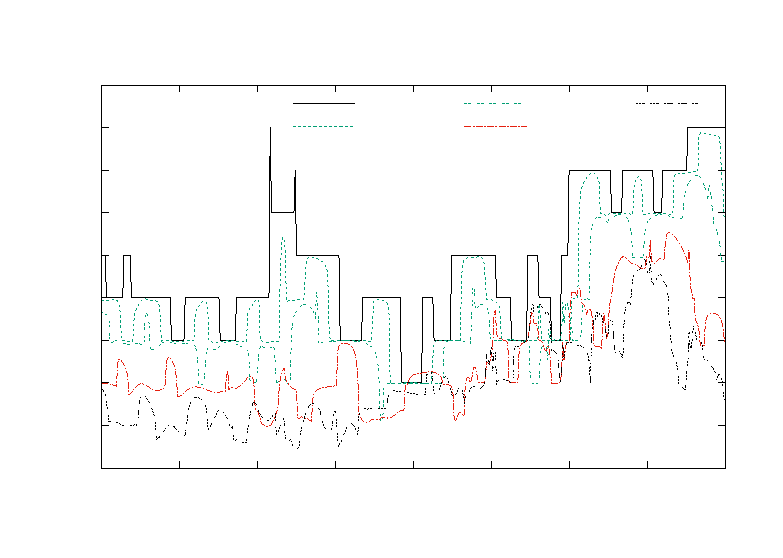
\includegraphics[width={360.00bp},height={252.00bp}]{zigzag-parallel-conductance-revise}}%
    \gplfronttext
  \end{picture}%
\endgroup
}  
  \end{latin}
\caption{الف) نمودار ‌بورفین با لبه آرمچیر با عرض 4 سلول برای مغناطش متفاوت الکترودها در پیکربندی AP. ب) رسم ‌بورفین با لبه آرمچیر، و عرض سلول 4 واحد، برای مغناطش متفاوت الکترودها در پیکربندی P. ج) نمودار ‌بورفین با لبه زیگزاگ، با عرض سلول 4 واحد، برای مغناطش متفاوت الکترودها در پیکربندی P. د) رسم ‌بورفین با لبه زیگزاگ و عرض سلول 4 واحد، برای مغناطش متفاوت الکترودها در پیکربندی AP.}
\label{fig:conductance}
\end{figure*}
\begin{figure*}[!ht]
  \begin{latin}
    \centering
    \resizebox{0.32\textwidth}{!}{% GNUPLOT: LaTeX picture with Postscript
\begin{latin}
\begingroup
  \makeatletter
  \providecommand\color[2][]{%
    \GenericError{(gnuplot) \space\space\space\@spaces}{%
      Package color not loaded in conjunction with
      terminal option `colourtext'%
    }{See the gnuplot documentation for explanation.%
    }{Either use 'blacktext' in gnuplot or load the package
      color.sty in LaTeX.}%
    \renewcommand\color[2][]{}%
  }%
  \providecommand\includegraphics[2][]{%
    \GenericError{(gnuplot) \space\space\space\@spaces}{%
      Package graphicx or graphics not loaded%
    }{See the gnuplot documentation for explanation.%
    }{The gnuplot epslatex terminal needs graphicx.sty or graphics.sty.}%
    \renewcommand\includegraphics[2][]{}%
  }%
  \providecommand\rotatebox[2]{#2}%
  \@ifundefined{ifGPcolor}{%
    \newif\ifGPcolor
    \GPcolorfalse
  }{}%
  \@ifundefined{ifGPblacktext}{%
    \newif\ifGPblacktext
    \GPblacktexttrue
  }{}%
  % define a \g@addto@macro without @ in the name:
  \let\gplgaddtomacro\g@addto@macro
  % define empty templates for all commands taking text:
  \gdef\gplbacktext{}%
  \gdef\gplfronttext{}%
  \makeatother
  \ifGPblacktext
    % no textcolor at all
    \def\colorrgb#1{}%
    \def\colorgray#1{}%
  \else
    % gray or color?
    \ifGPcolor
      \def\colorrgb#1{\color[rgb]{#1}}%
      \def\colorgray#1{\color[gray]{#1}}%
      \expandafter\def\csname LTw\endcsname{\color{white}}%
      \expandafter\def\csname LTb\endcsname{\color{black}}%
      \expandafter\def\csname LTa\endcsname{\color{black}}%
      \expandafter\def\csname LT0\endcsname{\color[rgb]{1,0,0}}%
      \expandafter\def\csname LT1\endcsname{\color[rgb]{0,1,0}}%
      \expandafter\def\csname LT2\endcsname{\color[rgb]{0,0,1}}%
      \expandafter\def\csname LT3\endcsname{\color[rgb]{1,0,1}}%
      \expandafter\def\csname LT4\endcsname{\color[rgb]{0,1,1}}%
      \expandafter\def\csname LT5\endcsname{\color[rgb]{1,1,0}}%
      \expandafter\def\csname LT6\endcsname{\color[rgb]{0,0,0}}%
      \expandafter\def\csname LT7\endcsname{\color[rgb]{1,0.3,0}}%
      \expandafter\def\csname LT8\endcsname{\color[rgb]{0.5,0.5,0.5}}%
    \else
      % gray
      \def\colorrgb#1{\color{black}}%
      \def\colorgray#1{\color[gray]{#1}}%
      \expandafter\def\csname LTw\endcsname{\color{white}}%
      \expandafter\def\csname LTb\endcsname{\color{black}}%
      \expandafter\def\csname LTa\endcsname{\color{black}}%
      \expandafter\def\csname LT0\endcsname{\color{black}}%
      \expandafter\def\csname LT1\endcsname{\color{black}}%
      \expandafter\def\csname LT2\endcsname{\color{black}}%
      \expandafter\def\csname LT3\endcsname{\color{black}}%
      \expandafter\def\csname LT4\endcsname{\color{black}}%
      \expandafter\def\csname LT5\endcsname{\color{black}}%
      \expandafter\def\csname LT6\endcsname{\color{black}}%
      \expandafter\def\csname LT7\endcsname{\color{black}}%
      \expandafter\def\csname LT8\endcsname{\color{black}}%
    \fi
  \fi
    \setlength{\unitlength}{0.0500bp}%
    \ifx\gptboxheight\undefined%
      \newlength{\gptboxheight}%
      \newlength{\gptboxwidth}%
      \newsavebox{\gptboxtext}%
    \fi%
    \setlength{\fboxrule}{0.5pt}%
    \setlength{\fboxsep}{1pt}%
\begin{picture}(3600.00,5040.00)%
    \gplgaddtomacro\gplbacktext{%
      \csname LTb\endcsname%%
      \put(1450,4200){\makebox(0,0)[r]{\strut{}$A$}}%
      \put(946,704){\makebox(0,0)[r]{\strut{}$-0.8$}}%
      \put(946,1439){\makebox(0,0)[r]{\strut{}$-0.7$}}%
      \put(946,2174){\makebox(0,0)[r]{\strut{}$-0.6$}}%
      \put(946,2909){\makebox(0,0)[r]{\strut{}$-0.5$}}%
      \put(946,3644){\makebox(0,0)[r]{\strut{}$-0.4$}}%
      \put(946,4379){\makebox(0,0)[r]{\strut{}$-0.3$}}%
      \put(1078,484){\makebox(0,0){\strut{}$0$}}%
      \put(1609,484){\makebox(0,0){\strut{}$0.5$}}%
      \put(2141,484){\makebox(0,0){\strut{}$1$}}%
      \put(2672,484){\makebox(0,0){\strut{}$1.5$}}%
      \put(3203,484){\makebox(0,0){\strut{}$2$}}%
      \put(1089,2909){\makebox(0,0)[l]{\strut{}$8\uparrow$}}%
      \put(1344,1439){\makebox(0,0)[l]{\strut{}$8\downarrow$}}%
      \put(1482,2909){\makebox(0,0)[l]{\strut{}$9\uparrow$}}%
      \put(1981,2174){\makebox(0,0)[l]{\strut{}$9\downarrow$}}%
    }%
    \gplgaddtomacro\gplfronttext{%
      \csname LTb\endcsname%%
      \put(209,2541){\rotatebox{-270}{\makebox(0,0){\strut{}$E(eV)$}}}%
      \put(2140,154){\makebox(0,0){\strut{}$k_x$}}%
      \csname LTb\endcsname%%
      \put(2140,4709){\makebox(0,0){\strut{}Left}}%
    }%
    \gplbacktext
    \put(0,0){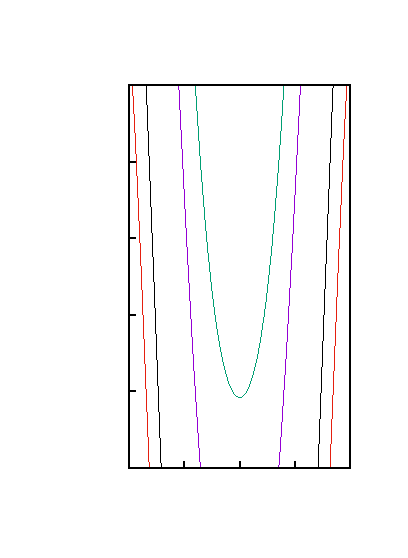
\includegraphics[width={180.00bp},height={252.00bp}]{Lborophene_band-revised}}%
    \gplfronttext
  \end{picture}%
\endgroup
\end{latin}}
    \resizebox{0.32\textwidth}{!}{% GNUPLOT: LaTeX picture with Postscript
\begin{latin}
\begingroup
  \makeatletter
  \providecommand\color[2][]{%
    \GenericError{(gnuplot) \space\space\space\@spaces}{%
      Package color not loaded in conjunction with
      terminal option `colourtext'%
    }{See the gnuplot documentation for explanation.%
    }{Either use 'blacktext' in gnuplot or load the package
      color.sty in LaTeX.}%
    \renewcommand\color[2][]{}%
  }%
  \providecommand\includegraphics[2][]{%
    \GenericError{(gnuplot) \space\space\space\@spaces}{%
      Package graphicx or graphics not loaded%
    }{See the gnuplot documentation for explanation.%
    }{The gnuplot epslatex terminal needs graphicx.sty or graphics.sty.}%
    \renewcommand\includegraphics[2][]{}%
  }%
  \providecommand\rotatebox[2]{#2}%
  \@ifundefined{ifGPcolor}{%
    \newif\ifGPcolor
    \GPcolorfalse
  }{}%
  \@ifundefined{ifGPblacktext}{%
    \newif\ifGPblacktext
    \GPblacktexttrue
  }{}%
  % define a \g@addto@macro without @ in the name:
  \let\gplgaddtomacro\g@addto@macro
  % define empty templates for all commands taking text:
  \gdef\gplbacktext{}%
  \gdef\gplfronttext{}%
  \makeatother
  \ifGPblacktext
    % no textcolor at all
    \def\colorrgb#1{}%
    \def\colorgray#1{}%
  \else
    % gray or color?
    \ifGPcolor
      \def\colorrgb#1{\color[rgb]{#1}}%
      \def\colorgray#1{\color[gray]{#1}}%
      \expandafter\def\csname LTw\endcsname{\color{white}}%
      \expandafter\def\csname LTb\endcsname{\color{black}}%
      \expandafter\def\csname LTa\endcsname{\color{black}}%
      \expandafter\def\csname LT0\endcsname{\color[rgb]{1,0,0}}%
      \expandafter\def\csname LT1\endcsname{\color[rgb]{0,1,0}}%
      \expandafter\def\csname LT2\endcsname{\color[rgb]{0,0,1}}%
      \expandafter\def\csname LT3\endcsname{\color[rgb]{1,0,1}}%
      \expandafter\def\csname LT4\endcsname{\color[rgb]{0,1,1}}%
      \expandafter\def\csname LT5\endcsname{\color[rgb]{1,1,0}}%
      \expandafter\def\csname LT6\endcsname{\color[rgb]{0,0,0}}%
      \expandafter\def\csname LT7\endcsname{\color[rgb]{1,0.3,0}}%
      \expandafter\def\csname LT8\endcsname{\color[rgb]{0.5,0.5,0.5}}%
    \else
      % gray
      \def\colorrgb#1{\color{black}}%
      \def\colorgray#1{\color[gray]{#1}}%
      \expandafter\def\csname LTw\endcsname{\color{white}}%
      \expandafter\def\csname LTb\endcsname{\color{black}}%
      \expandafter\def\csname LTa\endcsname{\color{black}}%
      \expandafter\def\csname LT0\endcsname{\color{black}}%
      \expandafter\def\csname LT1\endcsname{\color{black}}%
      \expandafter\def\csname LT2\endcsname{\color{black}}%
      \expandafter\def\csname LT3\endcsname{\color{black}}%
      \expandafter\def\csname LT4\endcsname{\color{black}}%
      \expandafter\def\csname LT5\endcsname{\color{black}}%
      \expandafter\def\csname LT6\endcsname{\color{black}}%
      \expandafter\def\csname LT7\endcsname{\color{black}}%
      \expandafter\def\csname LT8\endcsname{\color{black}}%
    \fi
  \fi
    \setlength{\unitlength}{0.0500bp}%
    \ifx\gptboxheight\undefined%
      \newlength{\gptboxheight}%
      \newlength{\gptboxwidth}%
      \newsavebox{\gptboxtext}%
    \fi%
    \setlength{\fboxrule}{0.5pt}%
    \setlength{\fboxsep}{1pt}%
\begin{picture}(3600.00,5040.00)%
    \gplgaddtomacro\gplbacktext{%
      \csname LTb\endcsname%%
      \put(1400,4200){\makebox(0,0)[r]{\strut{}$B$}}%
      \put(946,704){\makebox(0,0)[r]{\strut{}$-0.8$}}%
      \put(946,1439){\makebox(0,0)[r]{\strut{}$-0.7$}}%
      \put(946,2174){\makebox(0,0)[r]{\strut{}$-0.6$}}%
      \put(946,2909){\makebox(0,0)[r]{\strut{}$-0.5$}}%
      \put(946,3644){\makebox(0,0)[r]{\strut{}$-0.4$}}%
      \put(946,4379){\makebox(0,0)[r]{\strut{}$-0.3$}}%
      \put(1078,484){\makebox(0,0){\strut{}$0$}}%
      \put(1609,484){\makebox(0,0){\strut{}$0.5$}}%
      \put(2141,484){\makebox(0,0){\strut{}$1$}}%
      \put(2672,484){\makebox(0,0){\strut{}$1.5$}}%
      \put(3203,484){\makebox(0,0){\strut{}$2$}}%
      \put(1089,2909){\makebox(0,0)[l]{\strut{}$8\uparrow$}}%
      \put(1344,1439){\makebox(0,0)[l]{\strut{}$8\downarrow$}}%
      \put(1482,2909){\makebox(0,0)[l]{\strut{}$9\uparrow$}}%
      \put(1981,2174){\makebox(0,0)[l]{\strut{}$9\downarrow$}}%
    }%
    \gplgaddtomacro\gplfronttext{%
      \csname LTb\endcsname%%
      \put(209,2541){\rotatebox{-270}{\makebox(0,0){\strut{}$E(eV)$}}}%
      \put(2140,154){\makebox(0,0){\strut{}$k_x$}}%
      \csname LTb\endcsname%%
      \put(2140,4709){\makebox(0,0){\strut{}Center}}%
    }%
    \gplbacktext
    \put(0,0){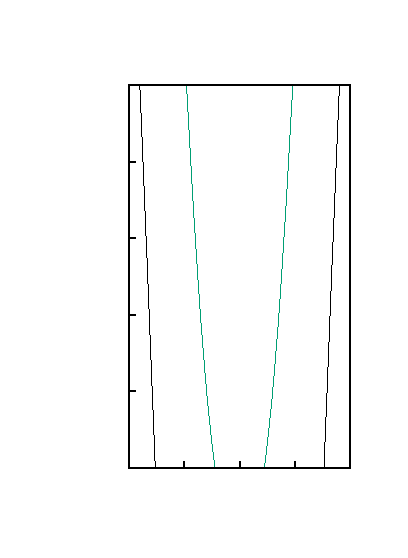
\includegraphics[width={180.00bp},height={252.00bp}]{Cborophene_band-revised}}%
    \gplfronttext
  \end{picture}%
\endgroup
\end{latin}}
    \resizebox{0.32\textwidth}{!}{% GNUPLOT: LaTeX picture with Postscript
\begingroup
  \makeatletter
  \providecommand\color[2][]{%
    \GenericError{(gnuplot) \space\space\space\@spaces}{%
      Package color not loaded in conjunction with
      terminal option `colourtext'%
    }{See the gnuplot documentation for explanation.%
    }{Either use 'blacktext' in gnuplot or load the package
      color.sty in LaTeX.}%
    \renewcommand\color[2][]{}%
  }%
  \providecommand\includegraphics[2][]{%
    \GenericError{(gnuplot) \space\space\space\@spaces}{%
      Package graphicx or graphics not loaded%
    }{See the gnuplot documentation for explanation.%
    }{The gnuplot epslatex terminal needs graphicx.sty or graphics.sty.}%
    \renewcommand\includegraphics[2][]{}%
  }%
  \providecommand\rotatebox[2]{#2}%
  \@ifundefined{ifGPcolor}{%
    \newif\ifGPcolor
    \GPcolorfalse
  }{}%
  \@ifundefined{ifGPblacktext}{%
    \newif\ifGPblacktext
    \GPblacktexttrue
  }{}%
  % define a \g@addto@macro without @ in the name:
  \let\gplgaddtomacro\g@addto@macro
  % define empty templates for all commands taking text:
  \gdef\gplbacktext{}%
  \gdef\gplfronttext{}%
  \makeatother
  \ifGPblacktext
    % no textcolor at all
    \def\colorrgb#1{}%
    \def\colorgray#1{}%
  \else
    % gray or color?
    \ifGPcolor
      \def\colorrgb#1{\color[rgb]{#1}}%
      \def\colorgray#1{\color[gray]{#1}}%
      \expandafter\def\csname LTw\endcsname{\color{white}}%
      \expandafter\def\csname LTb\endcsname{\color{black}}%
      \expandafter\def\csname LTa\endcsname{\color{black}}%
      \expandafter\def\csname LT0\endcsname{\color[rgb]{1,0,0}}%
      \expandafter\def\csname LT1\endcsname{\color[rgb]{0,1,0}}%
      \expandafter\def\csname LT2\endcsname{\color[rgb]{0,0,1}}%
      \expandafter\def\csname LT3\endcsname{\color[rgb]{1,0,1}}%
      \expandafter\def\csname LT4\endcsname{\color[rgb]{0,1,1}}%
      \expandafter\def\csname LT5\endcsname{\color[rgb]{1,1,0}}%
      \expandafter\def\csname LT6\endcsname{\color[rgb]{0,0,0}}%
      \expandafter\def\csname LT7\endcsname{\color[rgb]{1,0.3,0}}%
      \expandafter\def\csname LT8\endcsname{\color[rgb]{0.5,0.5,0.5}}%
    \else
      % gray
      \def\colorrgb#1{\color{black}}%
      \def\colorgray#1{\color[gray]{#1}}%
      \expandafter\def\csname LTw\endcsname{\color{white}}%
      \expandafter\def\csname LTb\endcsname{\color{black}}%
      \expandafter\def\csname LTa\endcsname{\color{black}}%
      \expandafter\def\csname LT0\endcsname{\color{black}}%
      \expandafter\def\csname LT1\endcsname{\color{black}}%
      \expandafter\def\csname LT2\endcsname{\color{black}}%
      \expandafter\def\csname LT3\endcsname{\color{black}}%
      \expandafter\def\csname LT4\endcsname{\color{black}}%
      \expandafter\def\csname LT5\endcsname{\color{black}}%
      \expandafter\def\csname LT6\endcsname{\color{black}}%
      \expandafter\def\csname LT7\endcsname{\color{black}}%
      \expandafter\def\csname LT8\endcsname{\color{black}}%
    \fi
  \fi
    \setlength{\unitlength}{0.0500bp}%
    \ifx\gptboxheight\undefined%
      \newlength{\gptboxheight}%
      \newlength{\gptboxwidth}%
      \newsavebox{\gptboxtext}%
    \fi%
    \setlength{\fboxrule}{0.5pt}%
    \setlength{\fboxsep}{1pt}%
\begin{picture}(3600.00,5040.00)%
    \gplgaddtomacro\gplbacktext{%
      \csname LTb\endcsname%%
      \put(1450,4200){\makebox(0,0)[r]{\strut{}$C$}}%
      \put(946,704){\makebox(0,0)[r]{\strut{}$-0.8$}}%
      \put(946,1439){\makebox(0,0)[r]{\strut{}$-0.7$}}%
      \put(946,2174){\makebox(0,0)[r]{\strut{}$-0.6$}}%
      \put(946,2909){\makebox(0,0)[r]{\strut{}$-0.5$}}%
      \put(946,3644){\makebox(0,0)[r]{\strut{}$-0.4$}}%
      \put(946,4379){\makebox(0,0)[r]{\strut{}$-0.3$}}%
      \put(1078,484){\makebox(0,0){\strut{}$0$}}%
      \put(1609,484){\makebox(0,0){\strut{}$0.5$}}%
      \put(2141,484){\makebox(0,0){\strut{}$1$}}%
      \put(2672,484){\makebox(0,0){\strut{}$1.5$}}%
      \put(3203,484){\makebox(0,0){\strut{}$2$}}%
      \put(1089,2909){\makebox(0,0)[l]{\strut{}$8\uparrow$}}%
      \put(1344,1439){\makebox(0,0)[l]{\strut{}$8\downarrow$}}%
      \put(1482,2909){\makebox(0,0)[l]{\strut{}$9\uparrow$}}%
      \put(1981,2174){\makebox(0,0)[l]{\strut{}$9\downarrow$}}%
    }%
    \gplgaddtomacro\gplfronttext{%
      \csname LTb\endcsname%%
      \put(209,2541){\rotatebox{-270}{\makebox(0,0){\strut{}$E(eV)$}}}%
      \put(2140,154){\makebox(0,0){\strut{}$k_x$}}%
      \csname LTb\endcsname%%
      \put(2140,4709){\makebox(0,0){\strut{}Right}}%
    }%
    \gplbacktext
    \put(0,0){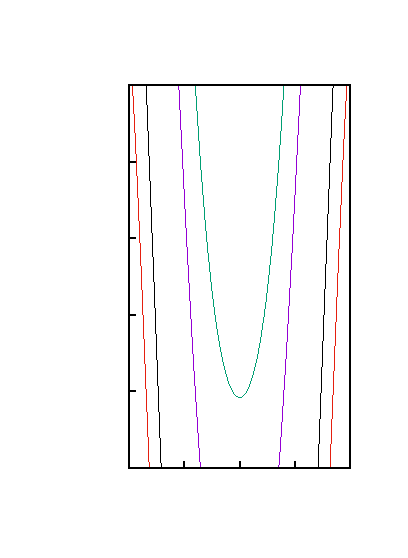
\includegraphics[width={180.00bp},height={252.00bp}]{Rborophene_band-revised}}%
    \gplfronttext
  \end{picture}%
\endgroup
}
    \resizebox{0.45\textwidth}{!}{% GNUPLOT: LaTeX picture with Postscript
\begin{latin}
\begingroup
  % Encoding inside the plot.  In the header of your document, this encoding
  % should to defined, e.g., by using
  % \usepackage[cp1252,<other encodings>]{inputenc}
  % \inputencoding{cp1252}%
  \makeatletter
  \providecommand\color[2][]{%
    \GenericError{(gnuplot) \space\space\space\@spaces}{%
      Package color not loaded in conjunction with
      terminal option `colourtext'%
    }{See the gnuplot documentation for explanation.%
    }{Either use 'blacktext' in gnuplot or load the package
      color.sty in LaTeX.}%
    \renewcommand\color[2][]{}%
  }%
  \providecommand\includegraphics[2][]{%
    \GenericError{(gnuplot) \space\space\space\@spaces}{%
      Package graphicx or graphics not loaded%
    }{See the gnuplot documentation for explanation.%
    }{The gnuplot epslatex terminal needs graphicx.sty or graphics.sty.}%
    \renewcommand\includegraphics[2][]{}%
  }%
  \providecommand\rotatebox[2]{#2}%
  \@ifundefined{ifGPcolor}{%
    \newif\ifGPcolor
    \GPcolorfalse
  }{}%
  \@ifundefined{ifGPblacktext}{%
    \newif\ifGPblacktext
    \GPblacktexttrue
  }{}%
  % define a \g@addto@macro without @ in the name:
  \let\gplgaddtomacro\g@addto@macro
  % define empty templates for all commands taking text:
  \gdef\gplbacktext{}%
  \gdef\gplfronttext{}%
  \makeatother
  \ifGPblacktext
    % no textcolor at all
    \def\colorrgb#1{}%
    \def\colorgray#1{}%
  \else
    % gray or color?
    \ifGPcolor
      \def\colorrgb#1{\color[rgb]{#1}}%
      \def\colorgray#1{\color[gray]{#1}}%
      \expandafter\def\csname LTw\endcsname{\color{white}}%
      \expandafter\def\csname LTb\endcsname{\color{black}}%
      \expandafter\def\csname LTa\endcsname{\color{black}}%
      \expandafter\def\csname LT0\endcsname{\color[rgb]{1,0,0}}%
      \expandafter\def\csname LT1\endcsname{\color[rgb]{0,1,0}}%
      \expandafter\def\csname LT2\endcsname{\color[rgb]{0,0,1}}%
      \expandafter\def\csname LT3\endcsname{\color[rgb]{1,0,1}}%
      \expandafter\def\csname LT4\endcsname{\color[rgb]{0,1,1}}%
      \expandafter\def\csname LT5\endcsname{\color[rgb]{1,1,0}}%
      \expandafter\def\csname LT6\endcsname{\color[rgb]{0,0,0}}%
      \expandafter\def\csname LT7\endcsname{\color[rgb]{1,0.3,0}}%
      \expandafter\def\csname LT8\endcsname{\color[rgb]{0.5,0.5,0.5}}%
    \else
      % gray
      \def\colorrgb#1{\color{black}}%
      \def\colorgray#1{\color[gray]{#1}}%
      \expandafter\def\csname LTw\endcsname{\color{white}}%
      \expandafter\def\csname LTb\endcsname{\color{black}}%
      \expandafter\def\csname LTa\endcsname{\color{black}}%
      \expandafter\def\csname LT0\endcsname{\color{black}}%
      \expandafter\def\csname LT1\endcsname{\color{black}}%
      \expandafter\def\csname LT2\endcsname{\color{black}}%
      \expandafter\def\csname LT3\endcsname{\color{black}}%
      \expandafter\def\csname LT4\endcsname{\color{black}}%
      \expandafter\def\csname LT5\endcsname{\color{black}}%
      \expandafter\def\csname LT6\endcsname{\color{black}}%
      \expandafter\def\csname LT7\endcsname{\color{black}}%
      \expandafter\def\csname LT8\endcsname{\color{black}}%
    \fi
  \fi
    \setlength{\unitlength}{0.0500bp}%
    \ifx\gptboxheight\undefined%
      \newlength{\gptboxheight}%
      \newlength{\gptboxwidth}%
      \newsavebox{\gptboxtext}%
    \fi%
    \setlength{\fboxrule}{0.5pt}%
    \setlength{\fboxsep}{1pt}%
\begin{picture}(7200.00,5040.00)%
    \gplgaddtomacro\gplbacktext{%
      \csname LTb\endcsname%%
      \put(1200,4200){\makebox(0,0)[r]{\strut{}$D$}}%
      \put(814,704){\makebox(0,0)[r]{\strut{}$1$}}%
      \put(814,1229){\makebox(0,0)[r]{\strut{}$1.5$}}%
      \put(814,1754){\makebox(0,0)[r]{\strut{}$2$}}%
      \put(814,2279){\makebox(0,0)[r]{\strut{}$2.5$}}%
      \put(814,2804){\makebox(0,0)[r]{\strut{}$3$}}%
      \put(814,3329){\makebox(0,0)[r]{\strut{}$3.5$}}%
      \put(814,3854){\makebox(0,0)[r]{\strut{}$4$}}%
      \put(814,4379){\makebox(0,0)[r]{\strut{}$4.5$}}%
      \put(946,484){\makebox(0,0){\strut{}$-1$}}%
      \put(2117,484){\makebox(0,0){\strut{}$-0.8$}}%
      \put(3289,484){\makebox(0,0){\strut{}$-0.6$}}%
      \put(4460,484){\makebox(0,0){\strut{}$-0.4$}}%
      \put(5632,484){\makebox(0,0){\strut{}$-0.2$}}%
      \put(6803,484){\makebox(0,0){\strut{}$0$}}%
    }%
    \gplgaddtomacro\gplfronttext{%
      \csname LTb\endcsname%%
      \put(209,2541){\rotatebox{-270}{\makebox(0,0){\strut{}$G(e^2/h)$}}}%
      \put(3874,154){\makebox(0,0){\strut{}$E(eV)$}}%
      \csname LTb\endcsname%%
      \put(2522,4206){\makebox(0,0)[r]{\strut{}$M=0$}}%
      \csname LTb\endcsname%%
      \put(2522,3986){\makebox(0,0)[r]{\strut{}$M=0.05$}}%
      \csname LTb\endcsname%%
      \put(4169,4206){\makebox(0,0)[r]{\strut{}$M=0.1$}}%
      \csname LTb\endcsname%%
      \put(4169,3986){\makebox(0,0)[r]{\strut{}$M=0.2$}}%
      \csname LTb\endcsname%%
      \put(5816,4206){\makebox(0,0)[r]{\strut{}$M=0.3$}}%
      \csname LTb\endcsname%%
      \put(3874,4709){\makebox(0,0){\strut{}Parallel}}%
    }%
    \gplbacktext
    \put(0,0){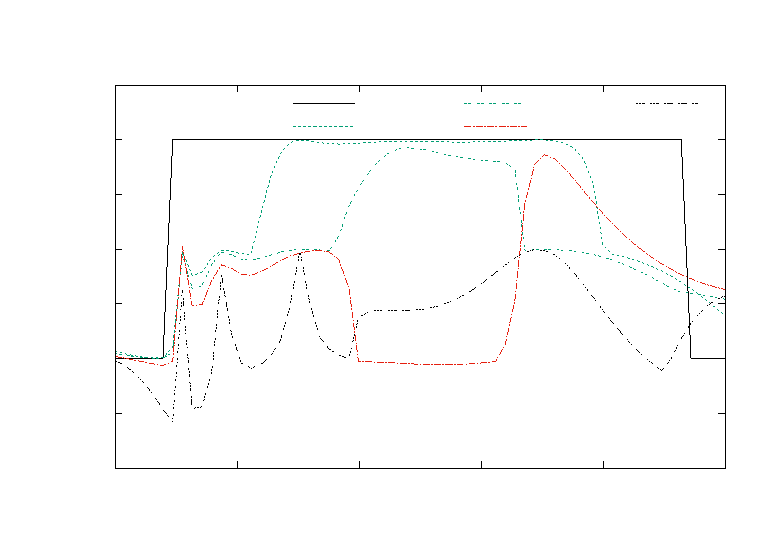
\includegraphics[width={360.00bp},height={252.00bp}]{armchair-parallel-conductance-1to0-revise}}%
    \gplfronttext
  \end{picture}%
\endgroup
\end{latin}}
    \resizebox{0.45\textwidth}{!}{\input{./figures/armchair-Antiparallel-conductance-1to0-revise.tex}}
  \end{latin}
\caption{الف, ب, ج) در الکترود سمت چپ، برای تعداد زوج اتم در سوپرسل، برای مثال، نوار شماره 8 (یا 9) با عدد اتم $8(9)$ مطابقت دارد که به دو زیر‌نوار اسپین بالا $ تقسیم ‌‌می‌‌شود. (8^\uparrow)$ و وقتی تعامل اسپین گنجانده شده است، $(8\downarrow)$ را به پایین بچرخانید: الف) در پیکربندی P، زیر‌نوارهای $(8\uparrow)$ در هر دو الکترود چپ و راست در بالای زیر‌نوارهای $(8\downarrow)$ با پاریته یکسان است و بنابراین ترابرد الکترون مجاز است. ب) در پیکربندی‌های AP، $(8\uparrow)$، در یک الکترود، بالاتر از زیر‌نوار $(8\downarrow)$ در همان الکترود قرار دارد، در حالی که در الکترود دیگر، $(8\uparrow)$ در زیر‌نوار $(8\downarrow)$ پایین تر با پاریته مخالف قرار دارد و بنابراین ترابرد الکترون مجاز نیست. د، ه) نمودار رسانایی در محدوده انرژی یکسان ساختار نواری برای پیکربندی‌های P و AP.}
\label{fig:bandconductance}
\end{figure*}

\begin{figure*}[!ht]
  \begin{latin}
    \centering
    \resizebox{0.45\textwidth}{!}{% GNUPLOT: LaTeX picture with Postscript
\begingroup
  % Encoding inside the plot.  In the header of your document, this encoding
  % should to defined, e.g., by using
  % \usepackage[cp1252,<other encodings>]{inputenc}
  % \inputencoding{cp1252}%
  \makeatletter
  \providecommand\color[2][]{%
    \GenericError{(gnuplot) \space\space\space\@spaces}{%
      Package color not loaded in conjunction with
      terminal option `colourtext'%
    }{See the gnuplot documentation for explanation.%
    }{Either use 'blacktext' in gnuplot or load the package
      color.sty in LaTeX.}%
    \renewcommand\color[2][]{}%
  }%
  \providecommand\includegraphics[2][]{%
    \GenericError{(gnuplot) \space\space\space\@spaces}{%
      Package graphicx or graphics not loaded%
    }{See the gnuplot documentation for explanation.%
    }{The gnuplot epslatex terminal needs graphicx.sty or graphics.sty.}%
    \renewcommand\includegraphics[2][]{}%
  }%
  \providecommand\rotatebox[2]{#2}%
  \@ifundefined{ifGPcolor}{%
    \newif\ifGPcolor
    \GPcolorfalse
  }{}%
  \@ifundefined{ifGPblacktext}{%
    \newif\ifGPblacktext
    \GPblacktexttrue
  }{}%
  % define a \g@addto@macro without @ in the name:
  \let\gplgaddtomacro\g@addto@macro
  % define empty templates for all commands taking text:
  \gdef\gplbacktext{}%
  \gdef\gplfronttext{}%
  \makeatother
  \ifGPblacktext
    % no textcolor at all
    \def\colorrgb#1{}%
    \def\colorgray#1{}%
  \else
    % gray or color?
    \ifGPcolor
      \def\colorrgb#1{\color[rgb]{#1}}%
      \def\colorgray#1{\color[gray]{#1}}%
      \expandafter\def\csname LTw\endcsname{\color{white}}%
      \expandafter\def\csname LTb\endcsname{\color{black}}%
      \expandafter\def\csname LTa\endcsname{\color{black}}%
      \expandafter\def\csname LT0\endcsname{\color[rgb]{1,0,0}}%
      \expandafter\def\csname LT1\endcsname{\color[rgb]{0,1,0}}%
      \expandafter\def\csname LT2\endcsname{\color[rgb]{0,0,1}}%
      \expandafter\def\csname LT3\endcsname{\color[rgb]{1,0,1}}%
      \expandafter\def\csname LT4\endcsname{\color[rgb]{0,1,1}}%
      \expandafter\def\csname LT5\endcsname{\color[rgb]{1,1,0}}%
      \expandafter\def\csname LT6\endcsname{\color[rgb]{0,0,0}}%
      \expandafter\def\csname LT7\endcsname{\color[rgb]{1,0.3,0}}%
      \expandafter\def\csname LT8\endcsname{\color[rgb]{0.5,0.5,0.5}}%
    \else
      % gray
      \def\colorrgb#1{\color{black}}%
      \def\colorgray#1{\color[gray]{#1}}%
      \expandafter\def\csname LTw\endcsname{\color{white}}%
      \expandafter\def\csname LTb\endcsname{\color{black}}%
      \expandafter\def\csname LTa\endcsname{\color{black}}%
      \expandafter\def\csname LT0\endcsname{\color{black}}%
      \expandafter\def\csname LT1\endcsname{\color{black}}%
      \expandafter\def\csname LT2\endcsname{\color{black}}%
      \expandafter\def\csname LT3\endcsname{\color{black}}%
      \expandafter\def\csname LT4\endcsname{\color{black}}%
      \expandafter\def\csname LT5\endcsname{\color{black}}%
      \expandafter\def\csname LT6\endcsname{\color{black}}%
      \expandafter\def\csname LT7\endcsname{\color{black}}%
      \expandafter\def\csname LT8\endcsname{\color{black}}%
    \fi
  \fi
    \setlength{\unitlength}{0.0500bp}%
    \ifx\gptboxheight\undefined%
      \newlength{\gptboxheight}%
      \newlength{\gptboxwidth}%
      \newsavebox{\gptboxtext}%
    \fi%
    \setlength{\fboxrule}{0.5pt}%
    \setlength{\fboxsep}{1pt}%
\begin{picture}(7200.00,5040.00)%
    \gplgaddtomacro\gplbacktext{%
      \csname LTb\endcsname%%
      \put(1400,4600){\makebox(0,0)[r]{\strut{}$A$}}%
      \put(814,1077){\makebox(0,0)[r]{\strut{}$0$}}%
      \put(814,1635){\makebox(0,0)[r]{\strut{}$0.2$}}%
      \put(814,2193){\makebox(0,0)[r]{\strut{}$0.4$}}%
      \put(814,2751){\makebox(0,0)[r]{\strut{}$0.6$}}%
      \put(814,3309){\makebox(0,0)[r]{\strut{}$0.8$}}%
      \put(814,3867){\makebox(0,0)[r]{\strut{}$1$}}%
      \put(946,857){\makebox(0,0){\strut{}$-4$}}%
      \put(1678,857){\makebox(0,0){\strut{}$-3$}}%
      \put(2410,857){\makebox(0,0){\strut{}$-2$}}%
      \put(3142,857){\makebox(0,0){\strut{}$-1$}}%
      \put(3875,857){\makebox(0,0){\strut{}$0$}}%
      \put(4607,857){\makebox(0,0){\strut{}$1$}}%
      \put(5339,857){\makebox(0,0){\strut{}$2$}}%
      \put(6071,857){\makebox(0,0){\strut{}$3$}}%
      \put(6803,857){\makebox(0,0){\strut{}$4$}}%
    }%
    \gplgaddtomacro\gplfronttext{%
      \csname LTb\endcsname%%
      \put(209,2541){\rotatebox{-270}{\makebox(0,0){\strut{}MR}}}%
      \put(3874,527){\makebox(0,0){\strut{}$E(eV)$}}%
      \csname LTb\endcsname%%
      \put(2654,4867){\makebox(0,0)[r]{\strut{}$M=0$}}%
      \csname LTb\endcsname%%
      \put(2654,4647){\makebox(0,0)[r]{\strut{}$M=0.05$}}%
      \csname LTb\endcsname%%
      \put(4301,4867){\makebox(0,0)[r]{\strut{}$M=0.1$}}%
      \csname LTb\endcsname%%
      \put(4301,4647){\makebox(0,0)[r]{\strut{}$M=0.2$}}%
      \csname LTb\endcsname%%
      \put(5948,4867){\makebox(0,0)[r]{\strut{}$M=0.3$}}%
    }%
    \gplbacktext
    \put(0,0){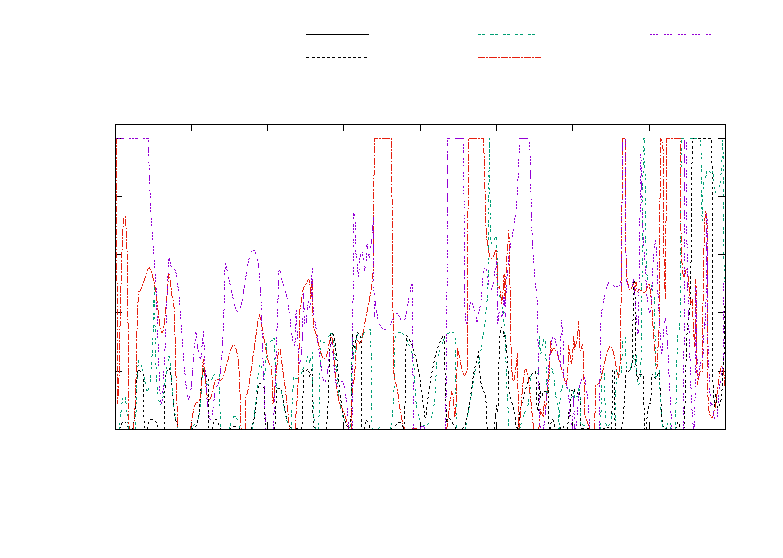
\includegraphics[width={360.00bp},height={252.00bp}]{MR-revise}}%
    \gplfronttext
  \end{picture}%
\endgroup
}
    \resizebox{0.45\textwidth}{!}{% GNUPLOT: LaTeX picture with Postscript
\begingroup
  % Encoding inside the plot.  In the header of your document, this encoding
  % should to defined, e.g., by using
  % \usepackage[cp1252,<other encodings>]{inputenc}
  % \inputencoding{cp1252}%s
  \makeatletter
  \providecommand\color[2][]{%
    \GenericError{(gnuplot) \space\space\space\@spaces}{%
      Package color not loaded in conjunction with
      terminal option `colourtext'%
    }{See the gnuplot documentation for explanation.%
    }{Either use 'blacktext' in gnuplot or load the package
      color.sty in LaTeX.}%
    \renewcommand\color[2][]{}%
  }%
  \providecommand\includegraphics[2][]{%
    \GenericError{(gnuplot) \space\space\space\@spaces}{%
      Package graphicx or graphics not loaded%
    }{See the gnuplot documentation for explanation.%
    }{The gnuplot epslatex terminal needs graphicx.sty or graphics.sty.}%
    \renewcommand\includegraphics[2][]{}%
  }%
  \providecommand\rotatebox[2]{#2}%
  \@ifundefined{ifGPcolor}{%
    \newif\ifGPcolor
    \GPcolorfalse
  }{}%
  \@ifundefined{ifGPblacktext}{%
    \newif\ifGPblacktext
    \GPblacktexttrue
  }{}%
  % define a \g@addto@macro without @ in the name:
  \let\gplgaddtomacro\g@addto@macro
  % define empty templates for all commands taking text:
  \gdef\gplbacktext{}%
  \gdef\gplfronttext{}%
  \makeatother
  \ifGPblacktext
    % no textcolor at all
    \def\colorrgb#1{}%
    \def\colorgray#1{}%
  \else
    % gray or color?
    \ifGPcolor
      \def\colorrgb#1{\color[rgb]{#1}}%
      \def\colorgray#1{\color[gray]{#1}}%
      \expandafter\def\csname LTw\endcsname{\color{white}}%
      \expandafter\def\csname LTb\endcsname{\color{black}}%
      \expandafter\def\csname LTa\endcsname{\color{black}}%
      \expandafter\def\csname LT0\endcsname{\color[rgb]{1,0,0}}%
      \expandafter\def\csname LT1\endcsname{\color[rgb]{0,1,0}}%
      \expandafter\def\csname LT2\endcsname{\color[rgb]{0,0,1}}%
      \expandafter\def\csname LT3\endcsname{\color[rgb]{1,0,1}}%
      \expandafter\def\csname LT4\endcsname{\color[rgb]{0,1,1}}%
      \expandafter\def\csname LT5\endcsname{\color[rgb]{1,1,0}}%
      \expandafter\def\csname LT6\endcsname{\color[rgb]{0,0,0}}%
      \expandafter\def\csname LT7\endcsname{\color[rgb]{1,0.3,0}}%
      \expandafter\def\csname LT8\endcsname{\color[rgb]{0.5,0.5,0.5}}%
    \else
      % gray
      \def\colorrgb#1{\color{black}}%
      \def\colorgray#1{\color[gray]{#1}}%
      \expandafter\def\csname LTw\endcsname{\color{white}}%
      \expandafter\def\csname LTb\endcsname{\color{black}}%
      \expandafter\def\csname LTa\endcsname{\color{black}}%
      \expandafter\def\csname LT0\endcsname{\color{black}}%
      \expandafter\def\csname LT1\endcsname{\color{black}}%
      \expandafter\def\csname LT2\endcsname{\color{black}}%
      \expandafter\def\csname LT3\endcsname{\color{black}}%
      \expandafter\def\csname LT4\endcsname{\color{black}}%
      \expandafter\def\csname LT5\endcsname{\color{black}}%
      \expandafter\def\csname LT6\endcsname{\color{black}}%
      \expandafter\def\csname LT7\endcsname{\color{black}}%
      \expandafter\def\csname LT8\endcsname{\color{black}}%
    \fi
  \fi
    \setlength{\unitlength}{0.0500bp}%
    \ifx\gptboxheight\undefined%
      \newlength{\gptboxheight}%
      \newlength{\gptboxwidth}%
      \newsavebox{\gptboxtext}%
    \fi%
    \setlength{\fboxrule}{0.5pt}%
    \setlength{\fboxsep}{1pt}%
\begin{picture}(7200.00,5040.00)%
    \gplgaddtomacro\gplbacktext{%
      \csname LTb\endcsname%%
      \put(1400,4600){\makebox(0,0)[r]{\strut{}$B$}}%
      \put(814,1077){\makebox(0,0)[r]{\strut{}$0$}}%
      \put(814,1635){\makebox(0,0)[r]{\strut{}$0.2$}}%
      \put(814,2193){\makebox(0,0)[r]{\strut{}$0.4$}}%
      \put(814,2751){\makebox(0,0)[r]{\strut{}$0.6$}}%
      \put(814,3309){\makebox(0,0)[r]{\strut{}$0.8$}}%
      \put(814,3867){\makebox(0,0)[r]{\strut{}$1$}}%
      \put(946,857){\makebox(0,0){\strut{}$-4$}}%
      \put(1678,857){\makebox(0,0){\strut{}$-3$}}%
      \put(2410,857){\makebox(0,0){\strut{}$-2$}}%
      \put(3142,857){\makebox(0,0){\strut{}$-1$}}%
      \put(3875,857){\makebox(0,0){\strut{}$0$}}%
      \put(4607,857){\makebox(0,0){\strut{}$1$}}%
      \put(5339,857){\makebox(0,0){\strut{}$2$}}%
      \put(6071,857){\makebox(0,0){\strut{}$3$}}%
      \put(6803,857){\makebox(0,0){\strut{}$4$}}%
    }%
    \gplgaddtomacro\gplfronttext{%
      \csname LTb\endcsname%%
      \put(209,2541){\rotatebox{-270}{\makebox(0,0){\strut{}MR}}}%
      \put(3874,527){\makebox(0,0){\strut{}$E(eV)$}}%
      \csname LTb\endcsname%%
      \put(2654,4867){\makebox(0,0)[r]{\strut{}$M=0$}}%
      \csname LTb\endcsname%%
      \put(2654,4647){\makebox(0,0)[r]{\strut{}$M=0.05$}}%
      \csname LTb\endcsname%%
      \put(4301,4867){\makebox(0,0)[r]{\strut{}$M=0.1$}}%
      \csname LTb\endcsname%%
      \put(4301,4647){\makebox(0,0)[r]{\strut{}$M=0.2$}}%
      \csname LTb\endcsname%%
      \put(5948,4867){\makebox(0,0)[r]{\strut{}$M=0.3$}}%
    }%
    \gplbacktext
    \put(0,0){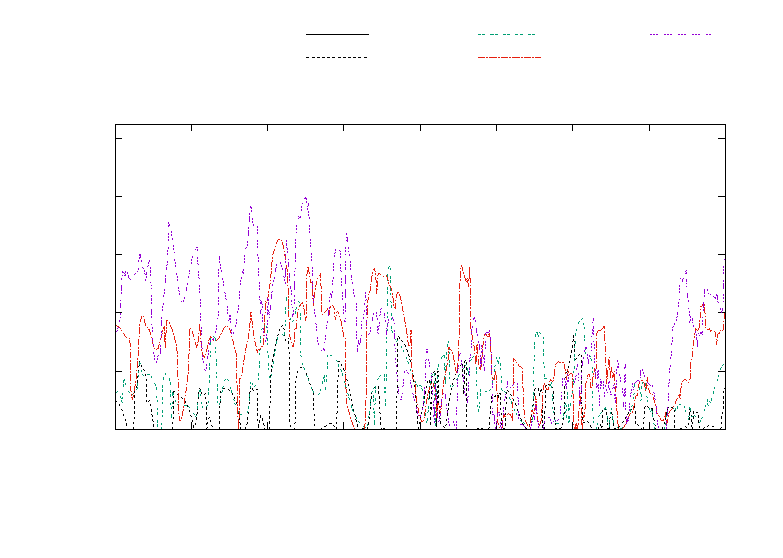
\includegraphics[width={360.00bp},height={252.00bp}]{MR_zig-revise}}%
    \gplfronttext
  \end{picture}%
\endgroup
}
  \end{latin}
\caption{مقاومت مغناطیس (MR) $\beta_{12}$-‌بورفین در آرمچیر راحتی و لبه‌های زیگزاگی.}
\label{fig:MR}
\end{figure*}

\begin{figure*}[!ht]
  \begin{latin}
    \centering
    \resizebox{0.45\textwidth}{!}{% GNUPLOT: LaTeX picture with Postscript
\begin{latin}
\begingroup
  % Encoding inside the plot.  In the header of your document, this encoding
  % should to defined, e.g., by using
  % \usepackage[cp1252,<other encodings>]{inputenc}
  % \inputencoding{cp1252}%
  \makeatletter
  \providecommand\color[2][]{%
    \GenericError{(gnuplot) \space\space\space\@spaces}{%
      Package color not loaded in conjunction with
      terminal option `colourtext'%
    }{See the gnuplot documentation for explanation.%
    }{Either use 'blacktext' in gnuplot or load the package
      color.sty in LaTeX.}%
    \renewcommand\color[2][]{}%
  }%
  \providecommand\includegraphics[2][]{%
    \GenericError{(gnuplot) \space\space\space\@spaces}{%
      Package graphicx or graphics not loaded%
    }{See the gnuplot documentation for explanation.%
    }{The gnuplot epslatex terminal needs graphicx.sty or graphics.sty.}%
    \renewcommand\includegraphics[2][]{}%
  }%
  \providecommand\rotatebox[2]{#2}%
  \@ifundefined{ifGPcolor}{%
    \newif\ifGPcolor
    \GPcolorfalse
  }{}%
  \@ifundefined{ifGPblacktext}{%
    \newif\ifGPblacktext
    \GPblacktexttrue
  }{}%
  % define a \g@addto@macro without @ in the name:
  \let\gplgaddtomacro\g@addto@macro
  % define empty templates for all commands taking text:
  \gdef\gplbacktext{}%
  \gdef\gplfronttext{}%
  \makeatother
  \ifGPblacktext
    % no textcolor at all
    \def\colorrgb#1{}%
    \def\colorgray#1{}%
  \else
    % gray or color?
    \ifGPcolor
      \def\colorrgb#1{\color[rgb]{#1}}%
      \def\colorgray#1{\color[gray]{#1}}%
      \expandafter\def\csname LTw\endcsname{\color{white}}%
      \expandafter\def\csname LTb\endcsname{\color{black}}%
      \expandafter\def\csname LTa\endcsname{\color{black}}%
      \expandafter\def\csname LT0\endcsname{\color[rgb]{1,0,0}}%
      \expandafter\def\csname LT1\endcsname{\color[rgb]{0,1,0}}%
      \expandafter\def\csname LT2\endcsname{\color[rgb]{0,0,1}}%
      \expandafter\def\csname LT3\endcsname{\color[rgb]{1,0,1}}%
      \expandafter\def\csname LT4\endcsname{\color[rgb]{0,1,1}}%
      \expandafter\def\csname LT5\endcsname{\color[rgb]{1,1,0}}%
      \expandafter\def\csname LT6\endcsname{\color[rgb]{0,0,0}}%
      \expandafter\def\csname LT7\endcsname{\color[rgb]{1,0.3,0}}%
      \expandafter\def\csname LT8\endcsname{\color[rgb]{0.5,0.5,0.5}}%
    \else
      % gray
      \def\colorrgb#1{\color{black}}%
      \def\colorgray#1{\color[gray]{#1}}%
      \expandafter\def\csname LTw\endcsname{\color{white}}%
      \expandafter\def\csname LTb\endcsname{\color{black}}%
      \expandafter\def\csname LTa\endcsname{\color{black}}%
      \expandafter\def\csname LT0\endcsname{\color{black}}%
      \expandafter\def\csname LT1\endcsname{\color{black}}%
      \expandafter\def\csname LT2\endcsname{\color{black}}%
      \expandafter\def\csname LT3\endcsname{\color{black}}%
      \expandafter\def\csname LT4\endcsname{\color{black}}%
      \expandafter\def\csname LT5\endcsname{\color{black}}%
      \expandafter\def\csname LT6\endcsname{\color{black}}%
      \expandafter\def\csname LT7\endcsname{\color{black}}%
      \expandafter\def\csname LT8\endcsname{\color{black}}%
    \fi
  \fi
    \setlength{\unitlength}{0.0500bp}%
    \ifx\gptboxheight\undefined%
      \newlength{\gptboxheight}%
      \newlength{\gptboxwidth}%
      \newsavebox{\gptboxtext}%
    \fi%
    \setlength{\fboxrule}{0.5pt}%
    \setlength{\fboxsep}{1pt}%
\begin{picture}(7200.00,5040.00)%
    \gplgaddtomacro\gplbacktext{%
      \csname LTb\endcsname%%
      \put(1300,4200){\makebox(0,0)[r]{\strut{}$A$}}%
      \put(946,704){\makebox(0,0)[r]{\strut{}$-0.3$}}%
      \put(946,1323){\makebox(0,0)[r]{\strut{}$-0.2$}}%
      \put(946,1942){\makebox(0,0)[r]{\strut{}$-0.1$}}%
      \put(946,2562){\makebox(0,0)[r]{\strut{}$0$}}%
      \put(946,3181){\makebox(0,0)[r]{\strut{}$0.1$}}%
      \put(946,3800){\makebox(0,0)[r]{\strut{}$0.2$}}%
      \put(946,4419){\makebox(0,0)[r]{\strut{}$0.3$}}%
      \put(1078,484){\makebox(0,0){\strut{}$0$}}%
      \put(2509,484){\makebox(0,0){\strut{}$0.5$}}%
      \put(3941,484){\makebox(0,0){\strut{}$1$}}%
      \put(5372,484){\makebox(0,0){\strut{}$1.5$}}%
      \put(6803,484){\makebox(0,0){\strut{}$2$}}%
    }%
    \gplgaddtomacro\gplfronttext{%
      \csname LTb\endcsname%%
      \put(209,2561){\rotatebox{-270}{\makebox(0,0){\strut{}$\tau/V$}}}%
      \put(3940,154){\makebox(0,0){\strut{}$\theta$}}%
      \csname LTb\endcsname%%
      \put(5816,4246){\makebox(0,0)[r]{\strut{}$M=0.05$}}%
      \csname LTb\endcsname%%
      \put(5816,4026){\makebox(0,0)[r]{\strut{}$M=0.10$}}%
      \csname LTb\endcsname%%
      \put(5816,3806){\makebox(0,0)[r]{\strut{}$M=0.20$}}%
      \csname LTb\endcsname%%
      \put(5816,3586){\makebox(0,0)[r]{\strut{}$M=0.30$}}%
      \csname LTb\endcsname%%
      \put(3940,4709){\makebox(0,0){\strut{}Spin Torque 2D}}%
    }%
    \gplbacktext
    \put(0,0){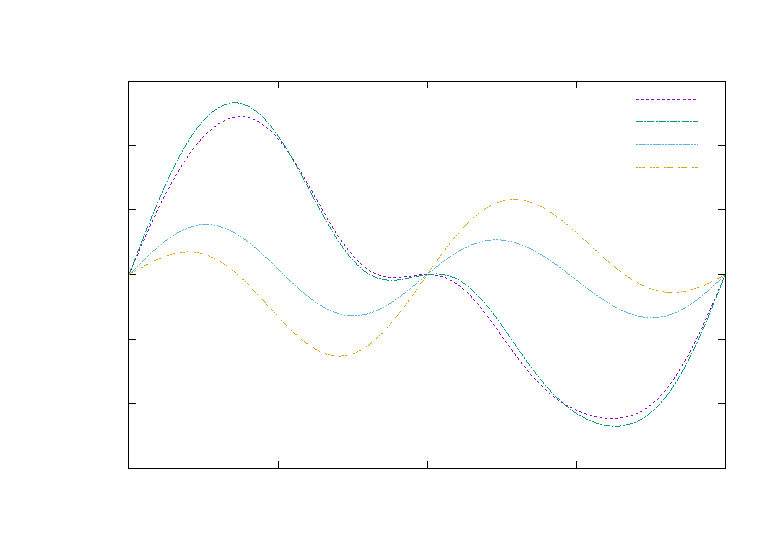
\includegraphics[width={360.00bp},height={252.00bp}]{stt}}%
    \gplfronttext
  \end{picture}%
\endgroup
\end{latin}}
    \resizebox{0.45\textwidth}{!}{% GNUPLOT: LaTeX picture with Postscript
\begingroup
  % Encoding inside the plot.  In the header of your document, this encoding
  % should to defined, e.g., by using
  % \usepackage[cp1252,<other encodings>]{inputenc}
  % \inputencoding{cp1252}%
  \makeatletter
  \providecommand\color[2][]{%
    \GenericError{(gnuplot) \space\space\space\@spaces}{%
      Package color not loaded in conjunction with
      terminal option `colourtext'%
    }{See the gnuplot documentation for explanation.%
    }{Either use 'blacktext' in gnuplot or load the package
      color.sty in LaTeX.}%
    \renewcommand\color[2][]{}%
  }%
  \providecommand\includegraphics[2][]{%
    \GenericError{(gnuplot) \space\space\space\@spaces}{%
      Package graphicx or graphics not loaded%
    }{See the gnuplot documentation for explanation.%
    }{The gnuplot epslatex terminal needs graphicx.sty or graphics.sty.}%
    \renewcommand\includegraphics[2][]{}%
  }%
  \providecommand\rotatebox[2]{#2}%
  \@ifundefined{ifGPcolor}{%
    \newif\ifGPcolor
    \GPcolorfalse
  }{}%
  \@ifundefined{ifGPblacktext}{%
    \newif\ifGPblacktext
    \GPblacktexttrue
  }{}%
  % define a \g@addto@macro without @ in the name:
  \let\gplgaddtomacro\g@addto@macro
  % define empty templates for all commands taking text:
  \gdef\gplbacktext{}%
  \gdef\gplfronttext{}%
  \makeatother
  \ifGPblacktext
    % no textcolor at all
    \def\colorrgb#1{}%
    \def\colorgray#1{}%
  \else
    % gray or color?
    \ifGPcolor
      \def\colorrgb#1{\color[rgb]{#1}}%
      \def\colorgray#1{\color[gray]{#1}}%
      \expandafter\def\csname LTw\endcsname{\color{white}}%
      \expandafter\def\csname LTb\endcsname{\color{black}}%
      \expandafter\def\csname LTa\endcsname{\color{black}}%
      \expandafter\def\csname LT0\endcsname{\color[rgb]{1,0,0}}%
      \expandafter\def\csname LT1\endcsname{\color[rgb]{0,1,0}}%
      \expandafter\def\csname LT2\endcsname{\color[rgb]{0,0,1}}%
      \expandafter\def\csname LT3\endcsname{\color[rgb]{1,0,1}}%
      \expandafter\def\csname LT4\endcsname{\color[rgb]{0,1,1}}%
      \expandafter\def\csname LT5\endcsname{\color[rgb]{1,1,0}}%
      \expandafter\def\csname LT6\endcsname{\color[rgb]{0,0,0}}%
      \expandafter\def\csname LT7\endcsname{\color[rgb]{1,0.3,0}}%
      \expandafter\def\csname LT8\endcsname{\color[rgb]{0.5,0.5,0.5}}%
    \else
      % gray
      \def\colorrgb#1{\color{black}}%
      \def\colorgray#1{\color[gray]{#1}}%
      \expandafter\def\csname LTw\endcsname{\color{white}}%
      \expandafter\def\csname LTb\endcsname{\color{black}}%
      \expandafter\def\csname LTa\endcsname{\color{black}}%
      \expandafter\def\csname LT0\endcsname{\color{black}}%
      \expandafter\def\csname LT1\endcsname{\color{black}}%
      \expandafter\def\csname LT2\endcsname{\color{black}}%
      \expandafter\def\csname LT3\endcsname{\color{black}}%
      \expandafter\def\csname LT4\endcsname{\color{black}}%
      \expandafter\def\csname LT5\endcsname{\color{black}}%
      \expandafter\def\csname LT6\endcsname{\color{black}}%
      \expandafter\def\csname LT7\endcsname{\color{black}}%
      \expandafter\def\csname LT8\endcsname{\color{black}}%
    \fi
  \fi
    \setlength{\unitlength}{0.0500bp}%
    \ifx\gptboxheight\undefined%
      \newlength{\gptboxheight}%
      \newlength{\gptboxwidth}%
      \newsavebox{\gptboxtext}%
    \fi%
    \setlength{\fboxrule}{0.5pt}%
    \setlength{\fboxsep}{1pt}%
\begin{picture}(7200.00,5040.00)%
    \gplgaddtomacro\gplbacktext{%
    }%
    \gplgaddtomacro\gplfronttext{%
      \csname LTb\endcsname%%
      \put(1300,3900){\makebox(0,0)[r]{\strut{}$B$}}%
      \put(936,674){\makebox(0,0){\strut{}$-4$}}%
      \put(1602,674){\makebox(0,0){\strut{}$-3$}}%
      \put(2268,674){\makebox(0,0){\strut{}$-2$}}%
      \put(2934,674){\makebox(0,0){\strut{}$-1$}}%
      \put(3600,674){\makebox(0,0){\strut{}$0$}}%
      \put(4266,674){\makebox(0,0){\strut{}$1$}}%
      \put(4932,674){\makebox(0,0){\strut{}$2$}}%
      \put(5598,674){\makebox(0,0){\strut{}$3$}}%
      \put(6264,674){\makebox(0,0){\strut{}$4$}}%
      \put(3600,344){\makebox(0,0){\strut{}$E(eV)$}}%
      \put(693,917){\makebox(0,0)[r]{\strut{}$-6$}}%
      \put(693,1318){\makebox(0,0)[r]{\strut{}$-4$}}%
      \put(693,1719){\makebox(0,0)[r]{\strut{}$-2$}}%
      \put(693,2120){\makebox(0,0)[r]{\strut{}$0$}}%
      \put(693,2520){\makebox(0,0)[r]{\strut{}$2$}}%
      \put(693,2920){\makebox(0,0)[r]{\strut{}$4$}}%
      \put(693,3321){\makebox(0,0)[r]{\strut{}$6$}}%
      \put(693,3722){\makebox(0,0)[r]{\strut{}$8$}}%
      \put(693,4123){\makebox(0,0)[r]{\strut{}$10$}}%
      \put(363,2520){\rotatebox{-270}{\makebox(0,0){\strut{}$\tau$}}}%
      \put(6795,917){\makebox(0,0)[l]{\strut{}$0$}}%
      \put(6795,1237){\makebox(0,0)[l]{\strut{}$0.2$}}%
      \put(6795,1558){\makebox(0,0)[l]{\strut{}$0.4$}}%
      \put(6795,1878){\makebox(0,0)[l]{\strut{}$0.6$}}%
      \put(6795,2199){\makebox(0,0)[l]{\strut{}$0.8$}}%
      \put(6795,2520){\makebox(0,0)[l]{\strut{}$1$}}%
      \put(6795,2840){\makebox(0,0)[l]{\strut{}$1.2$}}%
      \put(6795,3161){\makebox(0,0)[l]{\strut{}$1.4$}}%
      \put(6795,3481){\makebox(0,0)[l]{\strut{}$1.6$}}%
      \put(6795,3802){\makebox(0,0)[l]{\strut{}$1.8$}}%
      \put(6795,4123){\makebox(0,0)[l]{\strut{}$2$}}%
      \put(7257,2520){\rotatebox{-270}{\makebox(0,0){\strut{}$\theta$}}}%
      \put(3600,4453){\makebox(0,0){\strut{}$M=0.1$}}%
    }%
    \gplbacktext
    \put(0,0){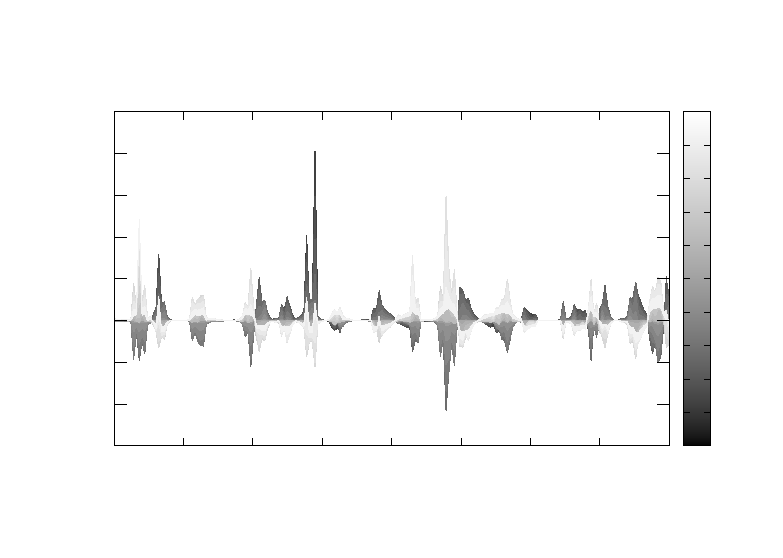
\includegraphics[width={360.00bp},height={252.00bp}]{stt-energy3d-0.1}}%
    \gplfronttext
  \end{picture}%
\endgroup
}
    \resizebox{0.45\textwidth}{!}{% GNUPLOT: LaTeX picture with Postscript
\begingroup
  % Encoding inside the plot.  In the header of your document, this encoding
  % should to defined, e.g., by using
  % \usepackage[cp1252,<other encodings>]{inputenc}
  % \inputencoding{cp1252}%
  \makeatletter
  \providecommand\color[2][]{%
    \GenericError{(gnuplot) \space\space\space\@spaces}{%
      Package color not loaded in conjunction with
      terminal option `colourtext'%
    }{See the gnuplot documentation for explanation.%
    }{Either use 'blacktext' in gnuplot or load the package
      color.sty in LaTeX.}%
    \renewcommand\color[2][]{}%
  }%
  \providecommand\includegraphics[2][]{%
    \GenericError{(gnuplot) \space\space\space\@spaces}{%
      Package graphicx or graphics not loaded%
    }{See the gnuplot documentation for explanation.%
    }{The gnuplot epslatex terminal needs graphicx.sty or graphics.sty.}%
    \renewcommand\includegraphics[2][]{}%
  }%
  \providecommand\rotatebox[2]{#2}%
  \@ifundefined{ifGPcolor}{%
    \newif\ifGPcolor
    \GPcolorfalse
  }{}%
  \@ifundefined{ifGPblacktext}{%
    \newif\ifGPblacktext
    \GPblacktexttrue
  }{}%
  % define a \g@addto@macro without @ in the name:
  \let\gplgaddtomacro\g@addto@macro
  % define empty templates for all commands taking text:
  \gdef\gplbacktext{}%
  \gdef\gplfronttext{}%
  \makeatother
  \ifGPblacktext
    % no textcolor at all
    \def\colorrgb#1{}%
    \def\colorgray#1{}%
  \else
    % gray or color?
    \ifGPcolor
      \def\colorrgb#1{\color[rgb]{#1}}%
      \def\colorgray#1{\color[gray]{#1}}%
      \expandafter\def\csname LTw\endcsname{\color{white}}%
      \expandafter\def\csname LTb\endcsname{\color{black}}%
      \expandafter\def\csname LTa\endcsname{\color{black}}%
      \expandafter\def\csname LT0\endcsname{\color[rgb]{1,0,0}}%
      \expandafter\def\csname LT1\endcsname{\color[rgb]{0,1,0}}%
      \expandafter\def\csname LT2\endcsname{\color[rgb]{0,0,1}}%
      \expandafter\def\csname LT3\endcsname{\color[rgb]{1,0,1}}%
      \expandafter\def\csname LT4\endcsname{\color[rgb]{0,1,1}}%
      \expandafter\def\csname LT5\endcsname{\color[rgb]{1,1,0}}%
      \expandafter\def\csname LT6\endcsname{\color[rgb]{0,0,0}}%
      \expandafter\def\csname LT7\endcsname{\color[rgb]{1,0.3,0}}%
      \expandafter\def\csname LT8\endcsname{\color[rgb]{0.5,0.5,0.5}}%
    \else
      % gray
      \def\colorrgb#1{\color{black}}%
      \def\colorgray#1{\color[gray]{#1}}%
      \expandafter\def\csname LTw\endcsname{\color{white}}%
      \expandafter\def\csname LTb\endcsname{\color{black}}%
      \expandafter\def\csname LTa\endcsname{\color{black}}%
      \expandafter\def\csname LT0\endcsname{\color{black}}%
      \expandafter\def\csname LT1\endcsname{\color{black}}%
      \expandafter\def\csname LT2\endcsname{\color{black}}%
      \expandafter\def\csname LT3\endcsname{\color{black}}%
      \expandafter\def\csname LT4\endcsname{\color{black}}%
      \expandafter\def\csname LT5\endcsname{\color{black}}%
      \expandafter\def\csname LT6\endcsname{\color{black}}%
      \expandafter\def\csname LT7\endcsname{\color{black}}%
      \expandafter\def\csname LT8\endcsname{\color{black}}%
    \fi
  \fi
    \setlength{\unitlength}{0.0500bp}%
    \ifx\gptboxheight\undefined%
      \newlength{\gptboxheight}%
      \newlength{\gptboxwidth}%
      \newsavebox{\gptboxtext}%
    \fi%
    \setlength{\fboxrule}{0.5pt}%
    \setlength{\fboxsep}{1pt}%
\begin{picture}(7200.00,5040.00)%
    \gplgaddtomacro\gplbacktext{%
    }%
    \gplgaddtomacro\gplfronttext{%
      \csname LTb\endcsname%%
      \put(1300,3900){\makebox(0,0)[r]{\strut{}$C$}}%
      \put(936,674){\makebox(0,0){\strut{}$-4$}}%
      \put(1602,674){\makebox(0,0){\strut{}$-3$}}%
      \put(2268,674){\makebox(0,0){\strut{}$-2$}}%
      \put(2934,674){\makebox(0,0){\strut{}$-1$}}%
      \put(3600,674){\makebox(0,0){\strut{}$0$}}%
      \put(4266,674){\makebox(0,0){\strut{}$1$}}%
      \put(4932,674){\makebox(0,0){\strut{}$2$}}%
      \put(5598,674){\makebox(0,0){\strut{}$3$}}%
      \put(6264,674){\makebox(0,0){\strut{}$4$}}%
      \put(3600,344){\makebox(0,0){\strut{}$E(eV)$}}%
      \put(693,917){\makebox(0,0)[r]{\strut{}$-4$}}%
      \put(693,1375){\makebox(0,0)[r]{\strut{}$-2$}}%
      \put(693,1833){\makebox(0,0)[r]{\strut{}$0$}}%
      \put(693,2291){\makebox(0,0)[r]{\strut{}$2$}}%
      \put(693,2749){\makebox(0,0)[r]{\strut{}$4$}}%
      \put(693,3207){\makebox(0,0)[r]{\strut{}$6$}}%
      \put(693,3665){\makebox(0,0)[r]{\strut{}$8$}}%
      \put(693,4123){\makebox(0,0)[r]{\strut{}$10$}}%
      \put(363,2520){\rotatebox{-270}{\makebox(0,0){\strut{}$\tau$}}}%
      \put(6795,917){\makebox(0,0)[l]{\strut{}$0$}}%
      \put(6795,1237){\makebox(0,0)[l]{\strut{}$0.2$}}%
      \put(6795,1558){\makebox(0,0)[l]{\strut{}$0.4$}}%
      \put(6795,1878){\makebox(0,0)[l]{\strut{}$0.6$}}%
      \put(6795,2199){\makebox(0,0)[l]{\strut{}$0.8$}}%
      \put(6795,2520){\makebox(0,0)[l]{\strut{}$1$}}%
      \put(6795,2840){\makebox(0,0)[l]{\strut{}$1.2$}}%
      \put(6795,3161){\makebox(0,0)[l]{\strut{}$1.4$}}%
      \put(6795,3481){\makebox(0,0)[l]{\strut{}$1.6$}}%
      \put(6795,3802){\makebox(0,0)[l]{\strut{}$1.8$}}%
      \put(6795,4123){\makebox(0,0)[l]{\strut{}$2$}}%
      \put(7257,2520){\rotatebox{-270}{\makebox(0,0){\strut{}$\theta$}}}%
      \put(3600,4453){\makebox(0,0){\strut{}$M=0.2$}}%
    }%
    \gplbacktext
    \put(0,0){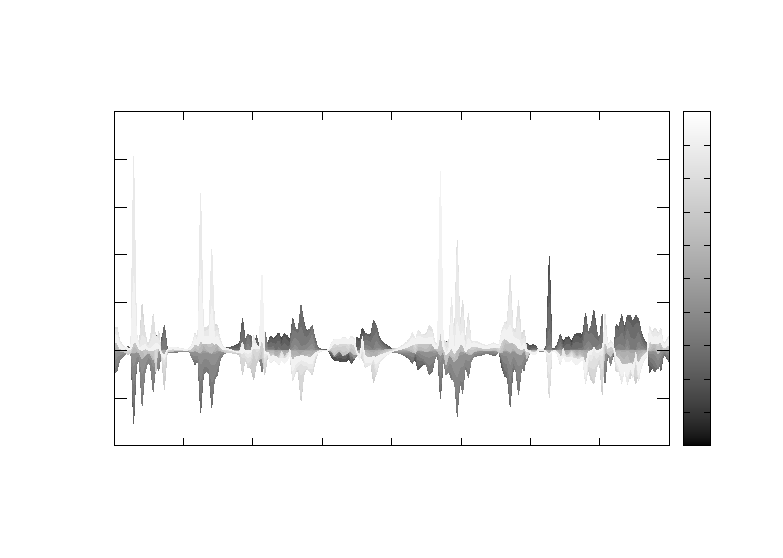
\includegraphics[width={360.00bp},height={252.00bp}]{stt-energy3d-0.2}}%
    \gplfronttext
  \end{picture}%
\endgroup
}
    \resizebox{0.45\textwidth}{!}{% GNUPLOT: LaTeX picture with Postscript
\begingroup
  % Encoding inside the plot.  In the header of your document, this encoding
  % should to defined, e.g., by using
  % \usepackage[cp1252,<other encodings>]{inputenc}
  % \inputencoding{cp1252}%
  \makeatletter
  \providecommand\color[2][]{%
    \GenericError{(gnuplot) \space\space\space\@spaces}{%
      Package color not loaded in conjunction with
      terminal option `colourtext'%
    }{See the gnuplot documentation for explanation.%
    }{Either use 'blacktext' in gnuplot or load the package
      color.sty in LaTeX.}%
    \renewcommand\color[2][]{}%
  }%
  \providecommand\includegraphics[2][]{%
    \GenericError{(gnuplot) \space\space\space\@spaces}{%
      Package graphicx or graphics not loaded%
    }{See the gnuplot documentation for explanation.%
    }{The gnuplot epslatex terminal needs graphicx.sty or graphics.sty.}%
    \renewcommand\includegraphics[2][]{}%
  }%
  \providecommand\rotatebox[2]{#2}%
  \@ifundefined{ifGPcolor}{%
    \newif\ifGPcolor
    \GPcolorfalse
  }{}%
  \@ifundefined{ifGPblacktext}{%
    \newif\ifGPblacktext
    \GPblacktexttrue
  }{}%
  % define a \g@addto@macro without @ in the name:
  \let\gplgaddtomacro\g@addto@macro
  % define empty templates for all commands taking text:
  \gdef\gplbacktext{}%
  \gdef\gplfronttext{}%
  \makeatother
  \ifGPblacktext
    % no textcolor at all
    \def\colorrgb#1{}%
    \def\colorgray#1{}%
  \else
    % gray or color?
    \ifGPcolor
      \def\colorrgb#1{\color[rgb]{#1}}%
      \def\colorgray#1{\color[gray]{#1}}%
      \expandafter\def\csname LTw\endcsname{\color{white}}%
      \expandafter\def\csname LTb\endcsname{\color{black}}%
      \expandafter\def\csname LTa\endcsname{\color{black}}%
      \expandafter\def\csname LT0\endcsname{\color[rgb]{1,0,0}}%
      \expandafter\def\csname LT1\endcsname{\color[rgb]{0,1,0}}%
      \expandafter\def\csname LT2\endcsname{\color[rgb]{0,0,1}}%
      \expandafter\def\csname LT3\endcsname{\color[rgb]{1,0,1}}%
      \expandafter\def\csname LT4\endcsname{\color[rgb]{0,1,1}}%
      \expandafter\def\csname LT5\endcsname{\color[rgb]{1,1,0}}%
      \expandafter\def\csname LT6\endcsname{\color[rgb]{0,0,0}}%
      \expandafter\def\csname LT7\endcsname{\color[rgb]{1,0.3,0}}%
      \expandafter\def\csname LT8\endcsname{\color[rgb]{0.5,0.5,0.5}}%
    \else
      % gray
      \def\colorrgb#1{\color{black}}%
      \def\colorgray#1{\color[gray]{#1}}%
      \expandafter\def\csname LTw\endcsname{\color{white}}%
      \expandafter\def\csname LTb\endcsname{\color{black}}%
      \expandafter\def\csname LTa\endcsname{\color{black}}%
      \expandafter\def\csname LT0\endcsname{\color{black}}%
      \expandafter\def\csname LT1\endcsname{\color{black}}%
      \expandafter\def\csname LT2\endcsname{\color{black}}%
      \expandafter\def\csname LT3\endcsname{\color{black}}%
      \expandafter\def\csname LT4\endcsname{\color{black}}%
      \expandafter\def\csname LT5\endcsname{\color{black}}%
      \expandafter\def\csname LT6\endcsname{\color{black}}%
      \expandafter\def\csname LT7\endcsname{\color{black}}%
      \expandafter\def\csname LT8\endcsname{\color{black}}%
    \fi
  \fi
    \setlength{\unitlength}{0.0500bp}%
    \ifx\gptboxheight\undefined%
      \newlength{\gptboxheight}%
      \newlength{\gptboxwidth}%
      \newsavebox{\gptboxtext}%
    \fi%
    \setlength{\fboxrule}{0.5pt}%
    \setlength{\fboxsep}{1pt}%
\begin{picture}(7200.00,5040.00)%
    \gplgaddtomacro\gplbacktext{%
    }%
    \gplgaddtomacro\gplfronttext{%
      \csname LTb\endcsname%%
      \put(1300,3900){\makebox(0,0)[r]{\strut{}$D$}}%
      \put(936,674){\makebox(0,0){\strut{}$-4$}}%
      \put(1602,674){\makebox(0,0){\strut{}$-3$}}%
      \put(2268,674){\makebox(0,0){\strut{}$-2$}}%
      \put(2934,674){\makebox(0,0){\strut{}$-1$}}%
      \put(3600,674){\makebox(0,0){\strut{}$0$}}%
      \put(4266,674){\makebox(0,0){\strut{}$1$}}%
      \put(4932,674){\makebox(0,0){\strut{}$2$}}%
      \put(5598,674){\makebox(0,0){\strut{}$3$}}%
      \put(6264,674){\makebox(0,0){\strut{}$4$}}%
      \put(3600,344){\makebox(0,0){\strut{}$E(eV)$}}%
      \put(693,917){\makebox(0,0)[r]{\strut{}$-6$}}%
      \put(693,1375){\makebox(0,0)[r]{\strut{}$-4$}}%
      \put(693,1833){\makebox(0,0)[r]{\strut{}$-2$}}%
      \put(693,2291){\makebox(0,0)[r]{\strut{}$0$}}%
      \put(693,2749){\makebox(0,0)[r]{\strut{}$2$}}%
      \put(693,3207){\makebox(0,0)[r]{\strut{}$4$}}%
      \put(693,3665){\makebox(0,0)[r]{\strut{}$6$}}%
      \put(693,4123){\makebox(0,0)[r]{\strut{}$8$}}%
      \put(363,2520){\rotatebox{-270}{\makebox(0,0){\strut{}$\tau$}}}%
      \put(6795,917){\makebox(0,0)[l]{\strut{}$0$}}%
      \put(6795,1237){\makebox(0,0)[l]{\strut{}$0.2$}}%
      \put(6795,1558){\makebox(0,0)[l]{\strut{}$0.4$}}%
      \put(6795,1878){\makebox(0,0)[l]{\strut{}$0.6$}}%
      \put(6795,2199){\makebox(0,0)[l]{\strut{}$0.8$}}%
      \put(6795,2520){\makebox(0,0)[l]{\strut{}$1$}}%
      \put(6795,2840){\makebox(0,0)[l]{\strut{}$1.2$}}%
      \put(6795,3161){\makebox(0,0)[l]{\strut{}$1.4$}}%
      \put(6795,3481){\makebox(0,0)[l]{\strut{}$1.6$}}%
      \put(6795,3802){\makebox(0,0)[l]{\strut{}$1.8$}}%
      \put(6795,4123){\makebox(0,0)[l]{\strut{}$2$}}%
      \put(7257,2520){\rotatebox{-270}{\makebox(0,0){\strut{}$\theta$}}}%
      \put(3600,4453){\makebox(0,0){\strut{}$M=0.3$}}%
    }%
    \gplbacktext
    \put(0,0){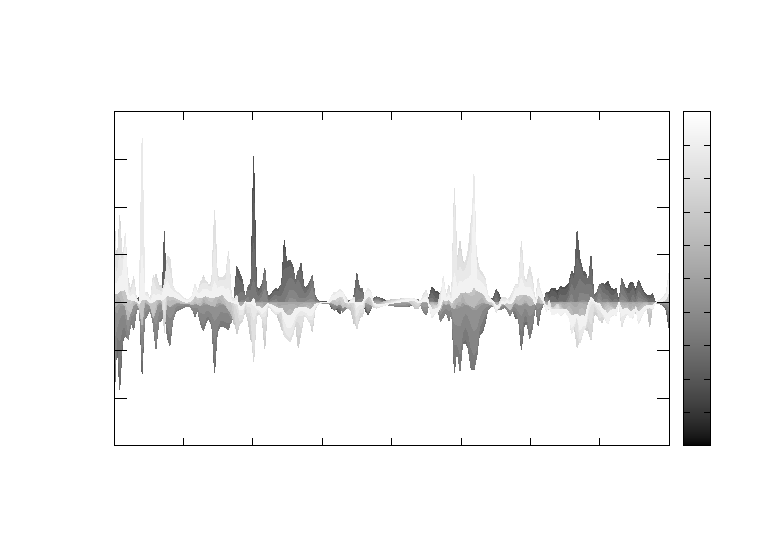
\includegraphics[width={360.00bp},height={252.00bp}]{stt-energy3d-0.3.eps}}%
    \gplfronttext
  \end{picture}%
\endgroup
}
  \end{latin}
    \caption{الف) گشتاور اسپینی از ‌بورفین با لبه آرمچیر، با عرض سلول 4 واحد، برای متغیر مغناطیسی الکترودها با توجه به درجه نسبی در جهت \lr{z} در \lr{E = 0 eV} ترسیم شده است. ب، ج، د) گشتاور اسپینی با مغناطش \lr{0.1، 0.2، 0.3 eV} نسبت به انرژی در تمام محدوده زوایای نسبی.}
    \label{fig:stt}
\end{figure*}


\section{اسپین‌ترونیک}
\gls{spintronic} معمولاً به پدیده‌هایی اطلاق ‌می‌‌شود که در آن اسپین الکترون‌ها در یک محیط حالت جامد نقش تعیین‌کننده را ایفا ‌می‌‌کند. به معنای محدودتر \gls{spintronic} یک ز‌مینه تحقیقاتی نوظهور در الکترونیک است. دستگاه‌های \gls{spintronic} بر اساس کنترل اسپین الکترون با کنترل الکتریکی و نوری اسپین یا مغناطیس هستند. در حالی که \gls{spintronic} فلزی قبلاً جایگاه خود را در صنعت رایانه پیدا کرده است. سیستم‌های مقاومت مغناطیسی غول‌پیکر به عنوان هدهای خواندن دیسک استفاده ‌می‌‌کنند، \gls{spintronic} نیمه‌رسانا هنوز پتانسیل کامل خود را نشان نداده است. اساسی‌ترین برهمکنش وابسته به اسپین در نیمه‌هادی‌های غیر مغناطیسی، جفت شدن اسپین-مدار است. بسته به تقارن‌های کریستالی مواد، و همچنین ویژگی‌های ساختاری هتروساختارها مبتنی بر نیمه‌رسانا، جفت‌شدگی مداری اسپین شکل‌های عملکردی متفاوتی به خود ‌می‌‌گیرد و ز‌مین بازی خوبی از همیلتونی‌های مدار اسپینی موثر ایجاد ‌می‌‌کند.‌ها‌میلتونی‌های مؤثر برای مرتبط‌ترین کلاس‌های مواد و ناهمساختارها در اینجا از توضیحات ساختار نوار الکترونیکی واقعی مشتق شده‌اند. 

اکثر سیستم‌های دستگاه‌های نیمه‌هادی هنوز مفاهیم نظری هستند و منتظر نمایش‌های تجربی هستند. مروری بر منتخب پیشنهادی، و چند دستگاه نشان‌داده‌شده، با شرح دقیق دو کلاس مهم ارائه ‌می‌‌شود: ساختارهای تونلی تشدید مغناطیسی و دیودها و ترانزیستورهای مغناطیسی دوقطبی.

\section{رسانش کوانتو‌‌می‌‌اسپین}

در بوروفین $\beta_{12}$ فقط چند مورد محاسبات دریچه اسپینی برای ساختار \gls{CIP} انجام شده است. خلأ این محاسبات مختلف، از جمله رسانندگی \gls{P} و \gls{AP} و \gls{MR} و \gls{STT}، در ساختار \lr{CPP} دریچه اسپینی برای $\beta_{12}$‌ بورفین احساس ‌می‌شود.این رساله به بررسی تحلیل نظری ترابرد وابسته به اسپین و ترابرد گشتاور اسپین برای  ساختار اتصال فرومغناطیس/نرمال/فرومغناطیس مبتنی بر ‌بورفین ‌می‌‌پردازد.  این مطالعه بر روی نانوریبان‌های ‌بورفین (\gls{BNR})ها به عنوان مبنایی برای محاسبات عددی دریچه اسپینی برای رسانندگی در هر دو پیکربندی که بردارهای مغناطیسی الکترودها موازی یا پاد‌موازی با یکدیگر هستند (به ترتیب پیکربندی‌های \gls{P} و \gls{AP})، مقاومت مغناطیسی (\gls{MR}) تمرکز ‌می‌کند. و گشتاور ترابرد اسپین (\gls{STT}). رویکردهای فرمالیسم \gls{Landauer} و تابع گرین غیرتعادلی (\gls{NEGF}) برای استخراج جریان‌های تونل زنی وابسته به اسپین در محل اتصال تونل مغناطیسی (\gls{MTJ}) استفاده ‌‌می‌‌شود. در اینجا ابتدا رسانایی ‌بورفین برای هر دو پیکربندی \gls{P} و \gls{AP} محاسبه ‌می‌شود و رسانایی صفر در برخی انرژی‌ها در پیکربندی \gls{AP} و رسانایی غیر صفر در پیکربندی \gls{P} مشاهده ‌می‌شود. این ویژگی حالت‌های روشن و خاموش را برای استفاده در کلید ایجاد ‌‌می‌‌کند. ترکیب پراکندگی وابسته به اسپین و فیلتر انتخاب نوار ممکن است دلیل رسانایی صفر را با استفاده از پاریته زیر‌نوارها در پیکربندی \gls{AP} را توضیح دهد.نتایج محاسبات برای \gls{BNR} زیگزاگ نشان ‌می‌دهد که رسانایی همیشه بزرگتر از $e^2/h$ برای پیکربندی \gls{P} مغناطیس‌های الکترود است. برای پیکربندی \gls{AP}، رسانایی در محدوده انرژی خاص صفر ‌‌می‌‌شود. یک فلات \gls{MR} کامل برای اتصال در غیاب بی نظ‌‌می‌‌ یافت ‌‌می‌‌شود، که ثابت ‌‌می‌‌کند کاندیدای عالی دریچه اسپینی است.تغییرات گشتاور ترابرد اسپین با انرژی فر‌‌می‌‌ و زاویه نسبی بین دو مغناطش الکترود در شدت‌های مغناطیسی فرومغناطیسی مختلف بررسی شده است. تغییرات \gls{STT} با انرژی فر‌‌می‌‌ و زاویه نسبی بین دو مغناطش الکترود، برای قدرت‌های مختلف مغناطش فرومغناطیسی مورد مطالعه قرار گرفته است. محاسبات نشان ‌‌می‌‌دهد که ولتاژ بایاس \gls{STT} در واحد $(e/4\pi)$، به عنوان تابعی از انرژی فر‌می‌، به طور قابل توجهی در نزدیکی انرژی نقطه دیراک کاهش ‌‌می‌‌یابد. علاوه بر این، یک الگوی نوسانی سینوسی را ‌‌می‌‌توان در \gls{STT} در ولتاژ بایاس واحد \lr{V} در مقابل زاویه بین دو مغناطش الکترود تشخیص داد که با افزایش \lr{M} تشدید ‌‌می‌‌شود. در نهایت، به منظور درک صحیح سیستم، \lr{G} به عنوان تابعی از زاویه نسبی بین دو مغناطش الکترود، و همچنین در اطراف انرژی نقطه دیراک بررسی ‌می‌شود.ولتاژ بایاس \gls{STT} ‌بورفین دارای خواص منحصر به فردی از جمله چگالی کم و سختی بالا، مقاومت در برابر حرارت و رسانایی الکتریکی است که آن را به یک نامزد ا‌میدوارکننده برای اسپین ترونیک تبدیل ‌‌می‌‌کند. این مقاله تجزیه و تحلیل جامعی از خواص ‌بورفین وابسته به اسپین و کاربردهای بالقوه آن در \gls{spintronic} ارائه ‌‌می‌‌دهد.

\section{دریچه‌اسپینی:}
یکی از پیشرفت‌های مهم در دو دهه اخیر، دریچه اسپینی  است، دستگاهی با دو اتصال مغناطیسی (شکل \ref{fig:spinvalve}) اگر در یک جهت مغناطیسی شوند (پیکربندی موازی، \gls{P})، مقاومت حاصل از مغناطیسی شدن آنها کمتر است. در جهت مخالف (پیکربندی پاد‌موازی، \gls{AP}). از زمان اولین نمایش خود در سال 1988، به سرعت به عنوان یک دستگاه خواندن برای درک اطلاعات ذخیره شده در یک حافظه مغناطیسی کاربرد پیدا کرد و این کشف با جایزه نوبل در سال 2007 شناخته شد.
\begin{figure*}[!ht]
  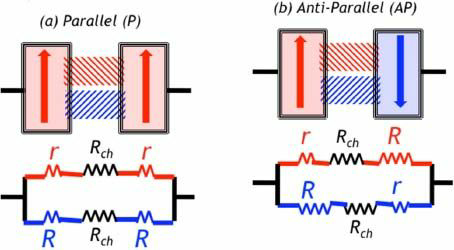
\includegraphics[width=1\linewidth]{./figures/spinvalve.png}
  \caption{دریچه اسپینی: (الف) پیکربندی موازی (P). (ب) پیکربندی پاد‌موازی (AP).}
  \label{fig:spinvalve}
\end{figure*}
تا اینجا ما فقط به اسپین به عنوان بخشی از "ضریب تبهگنی ، (\lr{g})" اشاره کرده‌ایم، ایده این است که حالت‌های الکترونیکی همیشه به صورت جفت ‌می‌‌آیند که یکی مربوط به هر اسپین است. همانطور که در شکل\ref{fig:spinvalve} انجام دادیم، ‌می‌‌توانیم اینها را «بالا» و «پایین» یا «چپ» و «راست» یا حتی «قرمز» و «آبی» بنا‌میم. توجه داشته باشید که این دو اسپین از نظر مکانی از هم جدا نیستند، حتی اگر کانال قرمز و آبی را برای وضوح از هم جدا کرد.

معمولاً دو کانال یکسان هستند و ‌‌می‌‌توانیم رسانایی ناشی از یک را محاسبه کنیم و به یاد داشته باشیم که در دو ضرب کنیم. اما در دستگاه‌های دریچه اسپین،اتصال‌ها مغناطیده هستند که با دو کانال اسپین برخورد متفاوتی ‌می‌‌کنند و عملکرد یک دریچه اسپینی با فرض اینکه که هر کانال اسپینی مقاومت رابط  متفاوتی، بسته به مغناطش اتصال، دارد،که یا موازی (اسپین اکثریت) یا پاد‌موازی (اسپین اقلیت) با مغناطش اتصال‌ها است.

اگر مقاومت رابط را برای اسپین‌های اکثریت r و برای اسپین‌های اقلیت $R \;(r < R)$ فرض کنیم، ‌‌می‌‌توانیم نمایش‌های مدار ساده‌ای را برای پیکربندی‌های \gls{P} و \gls{AP} همانطور که نشان داده شده است ترسیم کنیم، با $R_{ch}$ نشان دهنده مقاومت کانال است. سپس تئوری مدارهای ابتدایی مقاومت پیکربندی موازی را به ما ‌‌می‌‌دهد

همانطور که در شکل\ref{fig:model} نشان داده شده است، یک نانوروبان ‌بورفین غیر مغناطیسی (\gls{BNR}) با دو الکترود (به عنوان ناحیه مرکزی) که بین دو نانوروبان ‌بورفین \gls{FM} نیمه نامتناهی (به عنوان دو الکترود) قرار گرفته است، یک دستگاه \gls{spin valve} را تشکیل ‌‌می‌‌دهد. شایان ذکر است که حامل‌های بار ‌بورفین به طور کلی قطبش اسپینی نیستند و خاصیت مغناطیسی توسط یک بستر فرومغناطیسی عایق (با رشد ‌بورفین بر روی عایق \gls{FM}) به الکترودهای ‌بورفین تزریق ‌‌می‌‌شود. از آنجایی که استفاده از ‌میدان مغناطیسی ‌‌می‌‌تواند برای شکستن تقارن معکوس زمانی مورد استفاده قرار گیرد، ‌میدان تبادل ایجاد شده از طریق اثر مجاورت ناشی از یک بستر عایق فرومغناطیسی، باعث ‌‌می‌‌شود که زمان معکوس یا تقارن اسپین شکسته شود. بر خلاف روشهای جایگزین برای شکستن \lr{TRS}، مانند دوپینگ 79،80 اتم فلزات واسطه و حجم‌دهی  اتمی‌‌ 81،82، این تکنیک یک دستکاری برهمکنش کوتاه برد خارجی است که تأثیری بر تحرک الکترون در کاربردهای الکترونیکی ندارد. 

% اگر ناحیه هسته دارای طول \lr{L} و دارای \lr{N} اتم در عرض باشد، این ناحیه دارای $5 N (2L + 1)$ اتم است. مجموع‌ها‌می‌لتونی سیستم \gls{spin valve} به صورت زیر بدست ‌‌می‌‌آید:

% \begin{equation}
%   H= H_L + H_R + H_c + H_T,
% \end{equation}
% که
% \begin{equation}
% H_{L}=\sum\limits_{i\in L,\sigma }{\left( E_{L}+\sigma M_{L} \right)} a_{i\sigma }^{\dagger} a_{i\sigma }-\sum\limits_{i,i+\alpha \in L,\sigma}{\left( t_{\alpha } a_{i\sigma}^{\dagger} a_{i+\alpha \ \sigma }+H.c.\right)},
% \end{equation}
% \begin{equation}
% \begin{split}
% H_{R}=\sum_{i\in R,\sigma}{\left( E_{R}+\sigma M_{R} cos\phi M_{R}\sin \phi\right)} a_{i\sigma}^{\dagger} a_{i\sigma } \\
% -\sum_{i\in R,\sigma} t_{\alpha } a_{i\sigma}^{\dagger} a_{i+\alpha\sigma}+H.c.,
% \end{split}
% \end{equation}
% \begin{equation}
% H_{C}=\sum_{i\in \ C,\sigma }{{{E}_{C}}}a_{i\sigma }^{\dagger}{{a}_{i\sigma }}-\sum_{i,i+\alpha \in \ C,\sigma }{({{t}_{\alpha }}\ a_{i}^{\dagger }{{a}_{i+\alpha }}+H.c.)},
% \end{equation}
% \begin{equation}
% H_{T}=-\sum_{i\in \ C,i+\alpha \in L,R,\sigma}{{{t}_{\alpha }}}\ a_{i\sigma }^{\dagger }{{a}_{i+\alpha \ \sigma }}+H.c.,
% \end{equation}

% جایی که $E_L$، $E_R$ و $E_C$ به ترتیب انرژیهای موجود در نانوروبانهای ‌بورفین در الکترودهای چپ و راست و ناحیه مرکزی هستند که ‌می‌توانند با ولتاژ گیت تنظیم شوند، بسته به محل نقطه شبکه، همانطور که در جدول\ref{tbl:hoppingtable} نشان داده شده است.

\begin{equation}
  \begin{aligned}
  & P:{{\left[ \frac{1}{2r+{{R}_{ch}}}+\frac{1}{2R+{{R}_{ch}}} \right]}^{-1}} \\ 
 & AP:\frac{r+R+{{R}_{ch}}}{2}  
  \end{aligned}
\end{equation}

\begin{figure*}
  \centering
  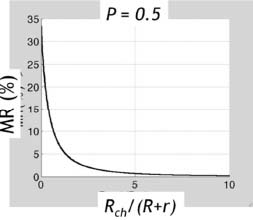
\includegraphics{./figures/MR-theory.png}
  \caption{تغییر در مقاومت مغناطیسی (\gls{MR}) به عنوان تابعی از مقاومت کانال نرمال شده است.}
  \label{fig:MRtheory}
\end{figure*}
ماهیت دستگاه دریچه اسپینی تفاوت بین $R_P$ و $R_{AP}$ .است 
% و ما انتظار داریم زمانی که مقاومت کانال ناچیز است و همه چیز تحت سلطه رابط‌ها است، این موضوع بیشتر برجسته باشد. شکل\ref{fig:MRtheory} تغییر مقاومت مغناطیسی (\gls{MR}، تعریف شده در زیر) را به عنوان تابعی از مقاومت کانال (در هر اسپین) $R_{ch}$ نرمال شده به $r+R$ با فرض $P=0.5$ نشان ‌می‌‌دهد. توجه داشته باشید که وقتی $R_{ch}$ نرمال شده بیش از مثلاً $~5$ افزایش یابد، \gls{MR} به سرعت از بین ‌‌می‌‌رود.

استفاده از مواد دوبعدی، گرافین و سیلیسین، به عنوان پایه برای شیرهای اسپینی بسیار مورد توجه قرار گرفته است. ‌بورفین به عنوان یکی دیگر از مواد دوبعدی با خواص جدیدش کمتر برای این منظور مورد مطالعه قرار گرفته است. در این رساله از ‌بورفین نیز برای همین منظور استفاده خواهیم کرد. با توجه به کاربردهای عملی متعدد در دستگاه‌هایی مانند کلید‌ها، هد‌هارد دیسک‌ها و \gls{MRAM}ها و همچنین \lr{STT-MRAM}‌ها و اهمیت پارامترهایی مانند رسانایی (موازی و پاد‌موازی)، \gls{MR} و \gls{STT} در طراحی یک \gls{spin valve}، مطالعه این خواص در ‌بورفین مورد توجه قرار خواهد گرفت. نتیجه محاسبات عددی برای \gls{CPP} برای پیکربندی‌های موازی (\gls{P})  و پاد‌موازی (\gls{AP})  متشکل از یک نانوروبان با عرض چهار سلول واحد در شکل\ref{fig:model} نشان داده شده است. در تمام محاسبات، الکترودهای چپ و راست به عنوان یک کانال ‌بورفین با مغناطیسی برابر، به صورت $M_L = M_R = M$ در نظر گرفته ‌‌می‌‌شوند. خاصیت مغناطیسی توسط یک بستر فرومغناطیسی عایق (با رشد ‌بورفین بر روی عایق \lr{FM}) به الکترودهای ‌بورفین تزریق ‌‌می‌‌شود. زاویه $\theta$ جهت گیری کلی مغناطش الکترودهای راست و چپ را نسبت به یکدیگر تعیین ‌‌می‌‌کند، در حالی که حالت خاص $\theta = 0 (\pi)$ به ترتیب مغناطش موازی (یا پاد‌موازی) الکترودهای چپ و راست را نشان ‌‌می‌‌دهد.

محاسبات ما نشان ‌‌می‌‌دهد که برخلاف \gls{ZBNR}‌ها، \gls{ABNR}ها رفتار نیمه‌هادی یا فلزی را بسته به عرض روبان $W$ از خود نشان ‌‌می‌‌دهند، به طوری که برای عرض‌های بزرگتر از مقدار بحرانی \AA $W_c = 11.08$، \cite{nikanEffectsEdgeDefects2022} رسانایی غیر صفر را ‌‌می‌‌توان یافت، در حالی که سیستم مانند یک نیمه‌هادی برای عرض‌های کوچکتر از $W_c$ رفتار ‌‌می‌‌کند. حالت‌های لبه را ‌‌می‌‌توان در شکاف انرژی نیمه‌هادی‌ها و همچنین شکاف نوار جایگزیده‌هادی‌ها مشاهده کرد. در نتیجه، حتی اگر معمولاً از نیمه‌هادی‌ها استفاده ‌‌می‌‌شود، حالت‌های صفر را ‌‌می‌‌توان در عرض‌های مشخص شده مناسب ایجاد کرد. اعمال ‌میدان مغناطیسی تبادل درون صفحه‌ای باعث ‌‌می‌‌شود‌ها‌میلتونین اسپین قطبی شده با عملگر اسپین \lr{S} جابجایی نداشته باشد و در این حالت اسپین الکترون دیگر ثابت حرکتی در سیستم نخواهد بود. این بدان معناست که حالت اسپین ممکن است در جهت انتقال تغییر کند. در واقع، در نتیجه برهمکنش اسپین الکترون با ‌میدان مغناطیسی تبادل درون صفحه، چرخش اسپین رخ ‌می‌دهد، به عنوان مثال، الکترونی که با حالت اسپین بالا وارد کانال ‌می‌شود ممکن است کانال را به صورت اسپین پایین ترک کند. 

هنگا‌‌می‌‌ که یک ‌میدان مغناطیسی به دلیل وجود یک زیرلایه عایق فرومغناطیسی روی الکترودها اعمال ‌‌می‌‌شود، یک ‌میدان مغناطیسی خارج از صفحه به شیرهای اسپین وارد ‌‌می‌‌شود. با توجه به بررسی‌های ما، در این مورد، رسانایی نسبت به الکترودهای غیر مغناطیسی تغییراتی را نشان ‌‌می‌‌دهد. تجزیه و تحلیل دقیق این تغییرات برای درک آنها و دانستن منشأ آنها یک مسئله که الکترودی برای طراحی شیرهای اسپین قابل اجرا و بهره برداری کامل از پتانسیل آنها است. 

در نتیجه تغییر خواص مغناطیسی الکترودها از حالت غیر مغناطیسی به مغناطیسی شده، تغییر در تعداد و عرض فلات‌ها ایجاد ‌‌می‌‌شود. با این حال، با افزایش مغناطش در الکترودها، انحراف از ساختار پله مانند به وضوح مشاهده ‌‌می‌‌شود. دلیل این امر را ‌‌می‌‌توان بر اساس خروج برخی از سطوح انرژی از پنجره انرژی ترابرد به دلیل جدا شدن سطوح انرژی در الکترودها به همراه حفظ پاریته زیرنوار انرژی به عنوان یکی از مکانیسم‌های دیگر مؤثر بر ترابرد بیان کرد. جداسازی اسپین ناشی از \gls{اثر زیمن}، ساختار نوار را تغییر ‌می‌‌دهد و در یک پنجره انرژی، تعداد زیر‌نوارها در هر دو حالت الکترودهای مغناطیسی و غیر مغناطیسی تغییر ‌می‌‌کند. در ادامه، انحرافات رسانایی در الکترودهای مغناطیسی شده را در مقایسه با غیر مغناطیسی شده توضیح ‌‌می‌‌دهیم که نمودارها رسانایی برای مغناطیس‌های مختلف $M$ را نشان ‌‌می‌‌دهند و آنها را با حالت $M = 0$ مقایسه ‌‌می‌‌کنند.

یکی از تغییرات از الکترودهای غیر مغناطیسی به حالت مغناطیسی، تغییر در تعداد و عرض صفحات در نمودار رسانندگی است که با افزایش مغناطیسی رخ ‌‌می‌‌دهد. فلات‌ها در نمودار ترابرد در محدوده انرژی دیده ‌‌می‌‌شوند که تعداد زیر‌نوارهای درگیر در فرآیند ترابرد ثابت است و زمانی که تعداد زیر‌نوارها در هر انرژی تغییر ‌‌می‌‌کند، رسانایی نیز تغییر ‌‌می‌‌کند. بنابراین، عرض پلاتوها در نمودار رسانایی به تفاوت بین زیر‌نوارهای انرژی بستگی دارد. با توجه به پایه دو  اتمی‌‌ موادی مانند گرافین، سیلیسن و غیره، فرورفتگی زیر‌نوارها حتی زمانی که تعامل تبادلی در نظر گرفته شود، رخ نمی‌‌دهد. دو نوع فاصله بین نواری دیده ‌‌می‌‌شود. اولی فاصله بین دو زیر‌نوار اسپینی با تراز مخالف یکسان است که برابر با $2M$ است و دیگری فاصله بین نوار اسپینی \lr{N - 1} و زیر‌نوار اسپینی \lr{N}ا‌مین است. در ‌بورفین، به دلیل وجود یک اتم اضافی که در مرکز شش ضلعی قرار دارد، سطح انرژی ناشی از برهمکنش تبادلی تورفتگی وجود دارد. به همین دلیل، تنوع فاصله بین زیر‌نوارها بسیار بیشتر از قبل است که با تنوع عرض پلاتوها همراه است و در رسانش شکل\ref{fig:conductance}(ب) نیز تایید شده است. بنابراین، برهمکنش مبادله به دلیل تغییری که در فاصله بین نوار ایجاد ‌‌می‌‌کند، الگوی رسانایی گام مانند را بیشتر تغییر ‌‌می‌‌دهد. 

یکی از اولین انحرافاتی که در الکترودهای مغناطیسی نشان داده شده در شکل\ref{fig:conductance}(الف,ب) در مقایسه با حالت غیر مغناطیسی یافت ‌‌می‌‌شود، وجود مراحل یا نوسانات در رسانایی با مقادیر کوچکتر از $G_0 (G_0 = e^2/h)$ در هر پیکربندی است. . علت این پدیده عدم تطابق بین پاریته زیر‌نوارهای کانال و پاریته زیر‌نوارهای الکترودهایی است که مقدار تونل آنها در مقایسه با حالت غیر مغناطیسی کمتر از یک $G_0$ است. این بدان معنی است که علاوه بر تعداد زیر‌نوارها در آن پنجره انرژی، پاریته زیر‌نوارها نیز در فرآیندهای تونل زنی و ترابرد الکترون بسیار مهم است. این متعاقبا باعث ایجاد فلات‌هایی با مقادیر فرد (که ‌‌می‌‌توان گفت دارای خواص نیمه فلزی هستند) یا مقادیر نیمه صحیح ‌‌می‌‌شود. البته برخلاف گرافین، این نوع تونل زنی الکترونی که در گرافین فقط در $E_F\le M$ دیده ‌‌می‌‌شود، در ‌بورفین در سراسر طیف انرژی دیده ‌‌می‌‌شود.
در غیاب هر گونه تعاملی که نرخ تونل زنی را کاهش دهد، با توجه به سهم  $G_0$ با توجه به هر زیر‌نوار در پنجره انرژی (همانطور که در مورد P مشاهده ‌‌می‌‌شود)، وجود هر فلات با ارتفاع $2G_0$ در نمودار هدایت، ‌میزان کل تونل زنی در پنجره انرژی را نشان ‌‌می‌‌دهد. در مورد \gls{AP}، سرعت کامل تونلزنی در دو موقعیت اتفاق نمی‌افتد:

1. وقتی دو زیر‌نوار مرتبط با دو الکترود پاریته مخالف دارند، علیرغم عدم وجود شکاف انرژی در ساختار نوار، رسانش صفر خواهد بود. در پیکربندی \gls{AP}، شماره گذاری نوارهای انرژی در الکترودهای چپ و راست با یکدیگر متفاوت است و پاریته نوارهای فرعی نیز مخالف است. یعنی زیر‌نوارهایی با اعداد یکسان در دو الکترود دارای پاریته مخالف هستند. در این صورت بر اساس قاعده انتخاب پاریته، تونل زنی ممنوع خواهد بود، یعنی در طول فرآیند تونل زنی، الکترون با پاریته زوج در الکترود چپ نمی‌‌تواند به الکترون با پاریته فرد در الکترود سمت راست تبدیل شود و بنابراین با وجود عدم وجود شکاف نوار، رسانایی صفر خواهد بود. (برای چنین الکترونی، حتی اگر شکاف نواری صفر باشد، رسانش باز هم صفر خواهد بود.) 

تعداد زیر‌نوارها به تعداد اتم‌های ابرسلول بستگی دارد و در غیاب ‌میدان مغناطیسی، دارای اسپین دوگانه هستند. انحطاط در الکترودها، زمانی که بستر مغناطیسی یک ‌میدان مغناطیسی به صفحه اعمال ‌‌می‌‌کند، تقسیم سطوح انرژی رخ ‌‌می‌‌دهد. بنابراین تعداد زیر‌نوارها دو برابر ‌‌می‌‌شود. از سوی دیگر، ‌‌می‌‌دانیم که زیر‌نوارها دارای تقارن پاریته به دلیل ساختار متقارن ماتریس $H_k$ هستند که به تعداد آنها بستگی دارد. یعنی زیر‌نوارهای 0، 2، 4 و . . . زوج هستند و زیر‌نوارهای 1، 3، 5 و . . . نیز عجیب و غریب هستند. وقتی زیر‌نوارها تقسیم ‌‌می‌‌شوند، این شماره گذاری دوباره از ابتدا انجام ‌‌می‌‌شود. بنابراین، در پیکربندی \gls{AP}، به عنوان مثال، زیر‌نوار 8 به دو نوار 8 به بالا و 8 پایین تقسیم ‌‌می‌‌شود که ترتیب آنها در الکترود مخالف برعکس است. با توجه به شماره گذاری مجدد به پاریته، زیر‌نوارهای با تعداد یکسان در دو الکترود با مغناطش مخالف، پاریته مخالف خواهند داشت و بنابراین در این حالت تونل سازی صورت نمی‌‌گیرد زیرا هر زمان که اسپین‌های زیر‌نوار در دو الکترود مخالف یکدیگر باشند، تونل زنی الکترونی ممنوع است. به یکدیگر. این بدان معناست که یک الکترون با پاریته زوج در الکترود چپ، در طول فرآیند تونلزنی، الکترون پاریته فرد را در الکترود سمت راست ایجاد نمی‌کند، که منجر به رسانایی صفر ‌می‌شود، حتی در صورت عدم وجود شکاف نواری در آن محدوده انرژی. 

2. در شرایطی که عدم تطابق پاریته در زیر‌نوارهای بین الکترودها و کانال مرکزی رخ ‌‌می‌‌دهد. در این حالت سهم تونل سازی در هر زیر‌نوار کمتر از $G_0$ و در نتیجه رسانایی کمتر از $2 G_0$ خواهد بود. مثلاً محدوده انرژی $-1 eV$ تا $0.0 eV$ برای $M = 0.3 eV$ در شکل\ref{fig:bandconductance}(ه). در برخی از انرژی‌ها در محدوده $-0.60 eV$ تا $-0.38 eV$، همانطور که در شکل\ref{fig:conductance}(الف) مشاهده ‌‌می‌‌شود، رسانایی برای $M = 0.2 eV$ صفر ‌‌می‌‌شود، با توجه به اینکه نمودار ساختار نواری هیچ شکاف نواری در این محدوده ندارد، همانطور که در شکل\ref{fig:bandconductance}(الف,ب,ج) مشاهده ‌‌می‌‌شود، دلیل رسانایی صفر را ‌‌می‌‌توان توضیح داد. بر اساس قوانین انتخاب پاریته در تونل زنی، در واقع، به طور دقیق تر، در این حالت، هماهنگی بین تعداد زیر‌نوارهای این پنجره انرژی و پاریته آنها به گونه‌ای است که این صفرهای رسانایی ایجاد ‌‌می‌‌شوند، اما لزوماً همه صفرهای رسانایی ایجاد نمی‌‌شوند. از این هماهنگی حاصل ‌‌می‌‌شود و این پنجره انرژی یک مثال است.

همچنین در یک \gls{ABNR} با پیکربندی \gls{P} حاوی چهار سلول واحد در عرض (شبیه به پیکربندی \gls{AP})، عرض فلات کاهش ‌‌می‌‌یابد و ساختار رسانایی پله مانند حفظ ‌‌می‌‌شود. رسانایی صفر در انرژی‌های $-0.6 eV$ و$0.38 eV$ و$0.63 eV$ تا $0.83 eV$ (برای $M = 0.2 eV$)، $0.35 eV$ تا $0.56 eV$ (برای $M = 0.3 eV$) دیگر رخ نمی‌‌دهد. همانطور که مشاهده ‌‌می‌‌شود، علیرغم شرایط مشابه در پیکربندی‌های \gls{P} و \gls{AP} شکل\ref{fig:bandconductance}(د,ه)(مانند نوع لبه‌ها، پنجره‌های انرژی و مغناطیس شدن الکترودها)، دلیل رسانایی غیر صفر در پیکربندی \gls{P} این است که برخلاف پیکربندی \gls{AP}، قانون انتخاب پاریته حفظ ‌‌می‌‌شود. 

البته، هنوز هم ‌‌می‌‌توان رفتار نیمه فلزی را برای این پیکربندی در انرژی‌های حدود $0.3 eV$ (با مغناطیسی $M = 0.3 eV$) و $-0.6 eV$ (با مغناطیسی $M = 0.2 eV$) در نظر گرفت. نوسانات کوچک در رسانایی شکل 2.c,d ناشی از عدم تطابق پاریته توابع موج عرضی در الکترودها و کانال است. در این حالت، ترابرد الکترون انجام ‌می‌شود، اما با سرعت کمتری نسبت به حالتی که پاریته دو نوار فرعی در الکترود و کانال یکسان است (که در مورد ما یک $G_0$ است).

نانوروبان‌های ‌بورفین زیگزاگ عموماً خواص رسانایی بیشتری از خود نشان ‌می‌دهند که با بررسی ساختار نواری آنها و مقایسه آن با نانوروبانهای ‌بورفین آرمچیر راحتی قابل مشاهده است. اگرچه نوسانات رسانایی را در اینجا نیز ‌‌می‌‌توان مشاهده کرد که ناشی از عدم تطابق پاریته حالات در الکترودها و کانال است، رسانایی با افزایش مغناطیس تغییرات زیادی را نشان ن‌‌می‌‌دهد. همچنین رسانایی صفر ظاهر نمی‌‌شود. تفاوت بین پیکربندی‌های \gls{P} و \gls{AP} در ‌بورفین زیگزاگ بسیار کمتر از ‌بورفین آرمچیر است، که متعاقباً باید به این نتیجه برسد که ‌بورفین زیگزاگ در دستگاه \gls{spin valve} ارزش کمتری خواهد داشت. بررسی \gls{MR} یک معیار مهم برای امکان استفاده از یک دستگاه به عنوان یک \gls{spin valve} مناسب فراهم ‌‌می‌‌کند. این بدان معناست که اگر یک دستگاه علاوه بر داشتن تغییرات قابل توجهی در رسانایی بین پیکربندیهای \gls{P} و \gls{AP} دارای مقاومت مغناطیسی بالایی باشد، ‌می‌تواند کاندیدای بالقوه خوبی برای یک دستگاه \gls{spin valve} باشد.

\section{مغناطومقاومت:}
اثر \gls{MR} را ‌‌می‌‌توان با استفاده از یک دستگاه \gls{spin valve} 12 تجزیه و تحلیل کرد. بسته به اینکه کانال ساندویچ شده در \gls{spin valve} فلزی یا عایق است، پدیده مقاومت مغناطیسی (\gls{GMR}) و مقاومت مغناطیسی تونل (\gls{TMR}) را ‌‌می‌‌توان مشاهده کرد. 13. علاوه بر توصیف فیزیک پشت رفتار \gls{MR}، بررسی نظری \gls{MR} همچنین نقش پارامترهای مختلف موثر در رفتار \gls{MR} \cite{harikumarNonEquilibriumGreenFunction2020} را مطالعه ‌می‌کند.

با توجه به تعریف \gls{MR}، بدیهی است که مقدار آن برای $M = 0 eV$ باید صفر باشد، زیرا در این حالت، هیچ تفاوتی بین تنظیمات \gls{AP} و \gls{P} وجود ندارد. در واقع مقادیر غیر صفر \lr{M} دو پیکربندی ذکر شده را از یکدیگر متمایز ‌‌می‌‌کند. همانطور که در شکل\ref{fig:MR}(الف) مشاهده ‌‌می‌‌شود، زمانی که $M = 0.05 eV$، یک ساختار فلات کامل را ‌‌می‌‌توان مشاهده کرد. در این مورد، پیکربندی پادموازی یک نارسانا با رسانایی صفر است، در حالی که پیکربندی موازی خواص رسانایی خوبی را با مقدار $G_0$ نشان ‌می‌دهد. 

ما ‌‌می‌‌دانیم که وقتی فلات‌های 100\% در نمودار \gls{MR} وجود دارد، رسانایی در \gls{AP} صفر ‌‌می‌‌شود و رسانایی برای پیکربندی \gls{P} به اندازه کافی بزرگ است، که از شکل\ref{fig:MR}(ب) مشخص است، که حدود یک $G_0$ است. در مقایسه با گرافین و سیلیسین، قله‌های \gls{MR} در ‌بورفین بسیار نامنظم تر و کمتر شبیه هیستوگرام هستند، همانطور که در شکل\ref{fig:MR}(الف) نشان داده شده است. برای $M = 0.05\; eV$، یک فلات 100٪ (فلات کامل) در انرژی $3.8\; eV$ رخ ‌‌می‌‌دهد که در آن عرض فلات با افزایش \lr{M} به $0.1\; eV$ افزایش ‌‌می‌‌یابد. که با دانش ما در مورد تغییر عرض فلات با \lr{M} مطابقت دارد.
همانطور که در شکل\ref{fig:conductance}(a) مشاهده ‌‌می‌‌شود، تعداد پنجره‌های انرژی با رسانایی صفر در پیکربندی \gls{AP} در $M = 0.2\; eV$ و $M = 0.3\; eV$ بسیار بیشتر است، و بنابراین تعداد فلات‌های 100\% نیز بیشتر است. 

برخلاف گرافین و سایر مواد دوبعدی، که فلات‌های 100 درصد (فلات کامل) در اطراف انرژی نقطه دیراک $E_F = 0\; eV$ قرار دارند، در ‌بورفین، فلات‌های 100 درصد در تمام انرژی‌ها رخ ‌‌می‌‌دهند و شکل هیستوگرام پایین تری را نشان ‌‌می‌‌دهند. این پدیده را ‌‌می‌‌توان یک مزیت برای ‌بورفین در نظر گرفت زیرا کاربرد مقاومت مغناطیسی گرافین در کلیدینگ به انرژی خاص (انرژی نقطه دیراک) محدود ‌‌می‌‌شود، در حالی که چنین محدودیتی برای ‌بورفین وجود ندارد. یعنی انتخاب‌های بیشتری در محدوده انرژی برای تنظیم سایر پارامترهای لازم برای ساخت دستگاه‌ها وجود دارد و ما محدود به انرژی خاصی نیستیم.

تغییر 100\% عرض فلات در ‌بورفین در درجه اول به دلیل رسانایی \gls{AP} صفر است، که متعاقباً بر اساس فاصله زیر‌نوارها و قانون انتخاب پاریته، همانطور که در بخش‌های قبلی بیان شد، به دست ‌‌می‌‌آید. از آنجایی که رسانایی دارای صفرهایی با عرض بزرگتر است (یعنی رسانایی در محدوده انرژی بزرگتر صفر است)، همان عرض انرژی با رسانایی صفر در نمودار \gls{MR} با فلات‌ها با مقدار یک $e^2/h$ منعکس ‌‌می‌‌شود. بنابراین، توصیف عرض فلات نمودار \gls{MR} کاملاً به دو عامل تعیین کننده صفرهای رسانایی بستگی دارد. 

علت دره‌ها در نمودار \gls{MR} به فاصله کمتر بین زیر‌نوارها در هر مغناطیس نسبت داده ‌‌می‌‌شود که منجر به نزدیک بودن رسانش در دو پیکربندی به یکدیگر ‌‌می‌‌شود. در نتیجه، ‌‌می‌‌توان نتیجه گرفت که رسانایی در آن نقاط تا حدودی مستقل از جهت گیری الکترودها است.
\section{ترابرد گشتاور اسپینی}
گشتاور ترابرد اسپین (\gls{STT}) به دلیل استفاده از اسپین الکترون در فناوری ذخیره سازی و حسگرها توجه بسیاری از محققین را به خود جلب کرده است. رالف و استایلز به صورت نظری فیزیک \gls{STT} را در دستگاه‌های مغناطیسی ارائه کردند. \gls{STT} با استفاده از مدل پخش اسپین  \cite{abertFieldandDampinglikeSpintransfer2017} و \gls{Zhang} و همکاران مکانیسم کلید مغناطیسی را با گنجاندن برهمکنش مبادله \cite{zhangMechanismsSpinpolarizedCurrentdriven2002} مورد بررسی قرار داد. 

با توجه به امکان استفاده از شیرهای اسپین در دستگاه‌های الکتریکی، مغناطیسی و اسپینی، مواد دوبعدی \lr{(2D)} در سال‌های بیشتر و بیشتر مورد توجه قرار گرفته اند. متغیرهای ساختاری متعددی، مانند اندازه پوسته، ضخامت، شکل لبه، عیوب ذاتی، اتمهای انتهایی لبه، و سایر متغیرهای، ‌می‌توانند بر ویژگی‌های یک ماده تأثیر بگذارند. قابلیت تبدیل مواد با لایه دوبعدی به نانوروبان‌ها، علاقه تحقیقاتی را برانگیخته است، زیرا این مواد به دلیل خواص مغناطیسی منحصر به فرد در ساختار الکترونیکی خود، پتانسیل تبدیل شدن به مواد الکترونیکی جدید را دارند. استفاده از نانو نوارها در الکترونیک اسپین یک موضوع تحقیقاتی رایج است. 

به دلیل ویژگی‌های استثنایی وابسته به اسپین، از جمله زمان واهلش اسپین فوق‌العاده طولانی و طول انتشار اسپین، جفتشدن مدار اسپینی راشبا \lr{(SOC)}، قفل شدن دره اسپینی، و اثر‌هال اسپین کوانتو‌می‌، مواد دوبعدی مانند گرافین \cite{novoselovElectricFieldEffect2004}، فسفر سیاه \lr{(BP)} \cite{liuPhosphoreneUnexplored2d2014}، دی کالکوژنیدهای فلزات واسطه \lr{(TMDCs)} \cite{wangElectronicsOptoelectronicsTwodimensional2012}، و سیلیسین \cite{guzman-verriElectronicStructureSiliconbased2007} یک پلتفرم عالی برای تحقیقات \gls{spintronic} ایجاد کرده اند.

\gls{Brey} و \gls{Fertig} \cite{breyMagnetoresistanceGraphenebasedSpin2007} \gls{MR} یک اتصال فرومغناطیس/نرمال/فرومغناطیس را در حد عرض بی نهایت با استفاده از مفهوم اتصال محکم بررسی کردند. از آنجایی که رسانایی به طور ضعیف تحت تأثیر جهت‌گیری‌های مغناطیسی نسبی سیم‌های \gls{FM} قرار ‌‌می‌‌گیرد، آنها دریافتند که \gls{MR} نسبتاً کم است. یک دستگاه قابل مقایسه با دو الکترود \gls{FM} توسط دینگ و همکاران مورد بررسی قرار گرفت. \cite{dingMagneticElectronicProperties2009} با استفاده از مدل پیوسته. 

بررسی تزریق اسپین به گرافین \cite{choSpinTransportPrecession2007, ohishiGiantMagnetoresistanceGraphene2007}، مقاومت مغناطیسی (\gls{MR}) \cite{wangQuantumTransportMassless2008}، گشتاور ترابرد اسپین ناشی از جریان \lr{(CISTT)} \cite{zhouMagnetotransportCurrentinducedSpin2010}، و تأثیر فیلتر اسپینی در دستگاههای مختلف مبتنی بر گرافین \cite{kangMagneticFieldDependence2011, shengElectronicTransportProperties2010} و غیره، نشان داده است. همچنین در تحقیقات مورد توجه بسیاری قرار گرفت. ترابرد وابسته به اسپین، مانند \gls{STT}، عمدتاً در مواد دوبعدی مانند گرافین، سیلیسین و سیلاگرافین در انتشارات قبلی \cite{maherSpindependentTransportSpin2022} مورد بررسی قرار گرفته است. 

‌بورفین، به عنوان یک لایه منفرد از اتم‌های بور، اخیراً به دلیل خواص منحصر به فردش، از جمله چگالی کم و سختی بالا، مقاومت در برابر حرارت (نقطه ذوب به طور قابل توجهی بالاتر از سیلیسن است) و رسانایی الکتریکی مورد توجه قرار گرفته است. 

‌بورفین به طور موثر بر روی بسترهای نقره، مس، نیکل و طلا سنتز شده است. برخی از خواص استثنایی آن، از جمله خواص مغناطیسی جدید الکتریکی، نوری، ترمودینا‌میکی، مکانیکی، و خاصیت ابررسانایی، قبلا مورد مطالعه قرار گرفته اند. اتم بور با اتم کربن در جدول تناوبی عناصر قابل مقایسه است. با این حال، بور دارای کلاس توپولوژیکی متفاوتی نسبت به کربن است به دلیل جفت شدن مدار اسپین پایین \lr{(SOC)} و الکترون‌های ظرفیت کمتر. در مورد گرافین، سیلیسن و سیلوگراف، محاسبات تقریباً کاملی برای ترابرد اسپین\cite{zhouSymmetrydependentSpinchargeTransport2015, maherSpindependentTransportSpin2022, chenElectronicTransportGraphenebased2010} انجام شده است. علاوه بر رسانایی در پیکربندیهای \gls{P} و \gls{AP} و همچنین زوایای نسبی دلخواه مغناطیس‌سازی الکترودها، محاسبات برای \gls{MR} و \gls{STT} در دستگاه شیر اسپین با ساختار \lr{CPP} نیز انجام شده و نتایج ارائه شده‌اند. 

ساختارهای مختلف مبتنی بر بور، از جمله خوشه‌ها، قفس‌های فولرن، نانولوله‌ها و ساختارهای دوبعدی \cite{wuTwoDimensionalBoronMonolayer2012, penevPolymorphismTwoDimensionalBoron2012, zhaiObservationAllboronFullerene2014}، که به‌عنوان نانوساختارهای $\alpha,\beta,\chi,\sigma$ طبقه‌بندی ‌می‌شوند، که $\beta_{12}$ و $\chi_{3}$ در حال حاضر به صورت تجربی سنتز شده‌اند، کشف شده‌اند. \cite{mannixSynthesisBorophenesAnisotropic2015, fengDirectEvidenceMetallic2016}. $\beta_{12}$ ‌بورفین، مانند گرافین و سیلیسین، دارای مخروط‌های دیراک با $p_z$ به عنوان یک مدار مهم است که مسئول خواص غیرمعمول الکترونیکی و ترابرد مواد \cite{tangNovelPrecursorsBoron2007} است. علاوه بر این، در توسعه صنعت الکترونیک، ‌بورفین تماس موثری با بسیاری از نیمه‌هادی‌های دوبعدی برقرار ‌‌می‌‌کند، مقاومت تماس را کاهش ‌‌می‌‌دهد و عملکرد ترانزیستورهای دوبعدی آینده را بهبود ‌‌می‌‌بخشد.

نسل بعدی شیرهای اسپینی، شیرهای اصلاح شده مبتنی بر گشتاور ترابرد اسپین (\gls{STT}) هستند که به دلیل پتانسیل آن در حافظه غیرفرار با مصرف برق نشتی نزدیک به صفر و ارائه فرصتهایی برای تک‌میل یا جایگزینی منطق بولین مبتنی بر \gls{CMOS}، ا‌میدوارکننده است. ، و از این رو، سزاوار بررسی و توجه بیشتر است. اگر مغناطش با زاویه‌ای به سمت چپ منحرف شود، الکترون‌های قطبی اسپینی که از چپ به الکترود \gls{FM} راست جریان دارند، ممکن است گشتاوری به نام گشتاور ترابرد اسپین (\gls{STT}) توالکترود کنند. به طور کلی \gls{STT} یک بردار است که ‌‌می‌‌تواند با استفاده از ولتاژهای بایاس کوچک به اجزای درون صفحه و خارج از صفحه تقسیم شود. مورد دوم بسیار کوچک است و ‌‌می‌‌توان آن را نادیده گرفت. 

تغییر گشتاور با $\theta$، همانطور که در شکل\ref{fig:stt}(الف) نشان داده شده است، ‌‌می‌‌تواند با یک تقریب خوب با مدلی شامل دو‌هارمونیک اول ارائه شده در زیر، با پارامترهای نشان داده شده در جدول\ref{tbl:fitting} برازش نمودار \lr{STT-$\theta$} با تابع $a\sin(\theta)+b\sin(2\theta)+c$ تنظیم ‌می‌‌شود. علاوه بر این، با افزایش $M$، $\tau_{x}/V$ نیز افزایش ‌می‌یابد، که تأیید ‌می‌کند که $\tau_{x}/V$ متناسب با قطبش \gls{FM}‌ها است.

همانطور که پیشبینی شد، گشتاور یک رفتار نوسان مانند از خود نشان ‌می‌دهد که مطابق با شبیه‌سازی‌های عددی قبلی برای گرافین \cite{maherSpindependentTransportSpin2022}، \cite{phamElectronicMagneticProperties2020}سیلیسین \cite{cheraghchiEdgeStatesTheir2012} و نقطه کوانتو‌‌می‌‌ است. این به این دلیل است که \gls{STT} با $M_R \times (M_L \times M_R)$ متناسب است و منجر به یک $\sin\theta$ ‌می‌شود. عامل. از این رو، گشتاور با تراز خطی $(\theta = 0, \pi)$ دو \gls{FM} ناپدید ‌‌می‌‌شود و با $M = 0\; eV$ به طور کامل ناپدید ‌‌می‌‌شود (در اینجا نشان داده نشده است). به نظر ‌‌می‌‌رسد که رفتار نوسان مانند در واقع یک رفتار سینوسی با‌هارمونیک‌های بیشتر در ‌بورفین است، در مقابل گرافین و سیلیسین که رفتاری کاملاً سینوسی دارند. 

در این منحنی، حداکثر مقدار گشتاور اسپین در جهت نسبی $61^\circ$ زمانی که مغناطش الکترودها$0.1\;eV$ باشد به دست ‌‌می‌‌آید. از سوی دیگر، به عنوان پارامتر برای \gls{STT} در مقابل در الکترودها افزایش ‌‌می‌‌یابد، مقدار گشتاور اسپین کاهش ‌‌می‌‌یابد. همچنین یک تقارن اسپینی حول محور وجود دارد. 

نمودار \gls{STT} در مقابل انرژی فر‌‌می‌‌ و زوایای نسبی الکترودها در شکل\ref{fig:stt}(ب) ارائه شده است. همانطور که انتظار ‌‌می‌‌رود، نمودار پیک‌هایی را نشان ‌‌می‌‌دهد که متناسب با تفاوت بین ارسال‌های اسپینی و اسپینی به پایین است. هر چه این اختلاف بزرگتر باشد، قله‌های تیزتر دیده ‌‌می‌‌شود و نقاط با \gls{STT} نزدیک به صفر نشان ‌‌می‌‌دهد که تفاوت بین ترابرد اسپین بالا و پایین بسیار کم است. 

در گرافین و سیلیسن، با دور شدن فرد از $E_F = 0\; eV$، پیک‌ها تیزتر ‌می‌‌شوند، که هم به دلیل نوسانات ترابرد اسپین در نزدیکی انرژی فر‌‌می‌‌ و هم به دلیل رفتار پله مانند در مناطق دور از انرژی فر‌‌می‌‌است. اما در ‌بورفین به دلیل فرورفتگی زیر‌نوارها این امر مشاهده نمی‌‌شود. ترابرد اسپین در ‌بورفین رفتارهای نوسانی و گام مانندی را به طور همزمان در مناطق مختلف نشان ‌‌می‌‌دهد. بنابراین پیک‌های \gls{STT} که بر اساس اختلاف ترابرد اسپین‌های بالا و پایین محاسبه ‌می‌شوند، رفتار مشابهی را نشان ‌می‌دهند. علاوه بر این، قله‌های بلند و کوتاه در کل محدوده انرژی دیده ‌‌می‌‌شود. 

اگرچه ممکن است نظم در منحنی \gls{STT} گرافین در ‌بورفین دیده نشود، اما از آنجایی که یکی از کاربردهای دستگاه‌های \gls{spin valve} جداسازی اسپین‌ها است، این تنوع و پراکندگی پیک‌ها، امکانات بیشتری را برای کنترل جداسازی اسپین فراهم ‌می‌کند. 

توانایی ترابرد اطلاعات اسپین ‌می‌تواند دستگاههای \gls{spintronic} پیچیده را فعال کند، مانند گیتهای منطقی قابل تنظیم مجدد که حافظه و منطق را یکپارچه ‌می‌کنند و راه را برای پردازش اطلاعات اسپینی هموار ‌می‌کنند. هر چند پارامترهای زیادی مانند تزریق و تشخیص و طول انتشار اسپین باید به طور همزمان قابل توجه و بهبود باشند تا در طراحی و ساخت دستگاه‌های پیچیده \gls{spintronic} موثر باشند، وجود انرژی‌هایی که در آن اسپین‌های بالا و پایین دارای طیف‌های مختلف انرژی هستند شرط لازم است. برای عملکرد دستگاه \cite{zhouSpindependentTransportCurrentinduced2016, seneorSpintronicsGraphene2012}. 

بنابراین وجود پیک‌های بیشتر در یک محدوده انرژی در نمودار \gls{STT} نشان دهنده انرژی‌هایی است که در آن اسپین‌های بالا و پایین از یکدیگر جدا ‌‌می‌‌شوند. همانطور که گفتیم برای استفاده از یک سیستم در ساخت و طراحی دستگاه‌های \gls{spintronic} باید شرایط زیادی تعیین شود که هر کدام ممکن است به انرژی بستگی داشته باشد. بنابراین، وجود پیکهایی که نشاندهنده جداسازی اسپین در انرژیهای مختلف است، ‌می‌تواند در کنترل سیستم برای انتخاب بهینهترین نقطه انرژی به منظور گسترش مطالعه یا طراحی ساخت دستگاههای \gls{spintronic} استفاده شود.

\begin{table}[t]
  \caption{ پارامتر برازش برای \gls{STT} در مقابل $\theta$}
  % \begin{latin}
    \centering
      \label{tbl:fitting}
      \begin{tabular}{cccc}
        \toprule
        M(eV) & a & b & c \\
        \midrule
        0.3 & 0.0649309- & 0.0726612 & 2.52642e-05 \\
        0.2 & 0.00900465 & 0.0655489 & 3.70375e-05- \\
        0.2 & 0.205575 & 0.0879828 & 0.00388147- \\
        0.05 & 0.200799 & 0.0728197 & 0.00673132- \\
        \bottomrule
      \end{tabular}
    % \end{latin}
  \end{table}
% \section{رسانش کوانتو‌‌می‌‌ در صفحات بروفین}
% \subsection{اصول و فرضيات:
% } یک مخروط دیراک در ساختار نواری ‌بورفین هیدروژنه (بوروفان) بین نقاط گاما و ایکس دیده ‌می‌‌شود، در مرجع[41].با مقایسه معادله دیراک برای ذرات با اسپین نیمه صحیح و‌ها‌میلتونی موثر بی جرم دو نوار انرژی صفحه که در انرژی‌های پایین معتبر است. همیلتونین مربوط به مخروط دیراک واقع در $k_d = (0.64،0،0 ±)^{-1}$\AA با معادله زیر آورده شده است:
% $$
% H_D = v_x \sigma_x p_x + v_y \sigma_y p_y + v_t I p_x
% $$

% جایی که $\sigma_x$ و $\sigma_y$ ماتریس‌های پاؤلی هستند و $I$ ماتریس یکانی به بعد 2 است. این عبارت یک مخروط دیراک \lr{2D} ناهمسانگرد کلی را تعریف ‌‌می‌‌کند ، که با سه ثابت $v_x$ ، $v_y$ , $v_t$ توصیف ‌‌می‌‌شود ، که به معنای سرعت در $x$ و $y$ است جهت و درجه شیب به ترتیب. قطری‌سازی این نتایج همیلتونین در پراکندگی انرژی است
% $$
% \epsilon(k_x,k_y) = (k_x - k_y) \pm \sqrt{(kx_ -k_y)^2 v_x^2 + k_y^2 v_y^2}
% $$

% طوری که $v_x = 19.58\times 10^5$ \lr{m / s} ، $v_y = 6.32\times 10^5$ \lr{m / s} ، $v_t = -5.06\times 10^5$ \lr{m / s}. یک نمودار کانتور از مخروط ناهمسانگرد دیراک در شکل 4 نشان داده شده است. سرعت در جهات $x$ مثبت و منفی به ترتیب توسط $v_x + | v_t | = 24.64 \times 10^5$  \lr{m / s} و $v_x - | v_t | = 14.52 \times 10^5$ متر در ثانیه $v_x + | v_t | ، v_x - | c_t|$ ، و $v_y$ برابر با $2.95$ ،$ 1.74$ و $0.76$ برابر سرعت فر‌‌می‌‌ گرافین هستند ($v_f =8.36\times 10^5$ \lr{m/s} ).[41]

% روش ماتریس انتقال مورد بررسی قرار گرفته است [45] در این تحقیق تلاش خواهیم کرد که نتایج استفاده از روش تابع گرین غیر تعادلی که در بخش پایانی به آن اشاره شده است را برای این سیستم بررسی نماییم. ‌‌می‌‌توانیم با استفاده از مدل تنگ بست با اضافه کردن اثرات مختلف به همیلتونی از طریق الگوریتم محاسباتی لوپز-سانشو اثر آن را روی ترابرد بررسی نماییم.
% \index{مثال}
% بررسی ترابرد دره‌ای در صفحات بروفین:
% در یک جامد بلوری ، رابطه بین انرژی الکترون و حرکت بلوری آن توسط ساختار نوار الکترونیکی ماده اداره ‌‌می‌‌شود. حداقل جایگزیده در نوار هدایت یا حداکثر جایگزیده در نوار ظرفیت به عنوان یک دره شناخته ‌‌می‌‌شود. علاوه بر شارژ و اسپین ، یک الکترون دارای درجه آزادی دره نیز ‌‌می‌‌باشد که دره‌ای را که الکترون اشغال ‌‌می‌‌کند مشخص ‌‌می‌‌کند. امکان استفاده از درجه آزادی دره برای ذخیره سازی و حمل اطلاعات (مشابه اسپین در اسپین‌ترونیک) منجر به کاربردهای الکترونیکی مفهو‌‌می‌‌‌‌ می‌‌شود که به عنوان \lr{valleytronics} [52-53]شناخته ‌‌می‌‌شوند. یک سیستم ماده ولیترونیک ایده آل دارای یک ساختار نوار متشکل از دو (یا بیشتر) دره تبهگن اما نابرابر (نقاط اکسترمم طیف انرژی جایگزیده) است که ‌‌می‌‌تواند برای رمزگذاری ، پردازش و ذخیره اطلاعات به‌کار گرفته شود.

% ایده بکارگیری درجه آزادی دره الکترونی چیز جدیدی نیست. به عنوان مثال ، کاملاً شناخته شده است که ‌‌می‌‌توان از کرنش برای تنظیم انرژی دره‌ها استفاده کرد ، که یک روش گسترده در صنعت الکترونیک نیمه‌هادی برای افزایش تحرکات حامل است.[54] در تحقیقات اساسی تر ، نیمه‌هادی‌های سنتی ، مانند سیلیکون و آلو‌مینیوم آرسنید \lr{(AlAs)} ، که دارای چندین دره در نوار‌های هدایت واقع در یا در نزدیکی نقاط تقارن \lr{X} در منطقه بریلوین هستند ، مورد بررسی قرار گرفته اند. کارهای اولیه بررسی درجه آزادی دره به دهه 1970 بر‌‌می‌‌گردد ، با مطالعاتی در مورد لایه‌های وارونگی در اتصال‌های سیلیکون/عایق [55؛56].

% در این مواد 2 بعدی شش ضلعی ، مانند گرافین و تک لایه گروه \lr{VI} که فلزی را ساندویچ کرده است.(\gls{TMD}‌ها) (به عنوان مثال \ce{MoS2} ، \ce{MoSe2} ، \ce{WS2} و \ce{WSe2}) ، ویژگی‌های الکترونیکی لبه نوار تحت سلطه دو دره ناموزون هستندکه در نقاط \lr{+K} و \lr{-K} در لبه‌های منطقه بریلوئن  قرار دارند.(شکل 4). این دره‌ها را ‌‌می‌‌توان با یک شبه اسپین دودویی نشان داد که مانند سیستم \lr{spin-1/2} رفتار ‌‌می‌‌کند. الکترونهای موجود در \lr{+K} ‌‌می‌‌توانند به عنوان شبه ذره اسپین بالا ، و الکترونهای موجود در دره \lr{-K} ‌‌می‌‌توانند به عنوان دراسپین پایین برچسب گذاری شوند. بنابراین ، در یک سیستم دوپینگ ، یک توزیع جمعیت حامل قطبی در یک دره \lr{+K} یا \lr{K} ‌‌می‌‌تواند اطلاعات باینری را ذخیره کند.

% اعمال ‌میدان الکتریکی در بخش باریک شکل فوق تراز فر‌‌می‌‌ را در این بازه جابجا ‌‌می‌‌کند. در اینصورت نمودار نوار انرژی در سه بخش مختلف نوار به شکل زیر در ‌می‌‌آید:

% در مرجع مذکور نشان داده شده است که با بالا بردن تراز فر‌‌می‌ ‌در محدوده کانال، الکترونهایی که دارای اندیس دره ی منفی هستند (دایره‌های تو خالی) به طور کامل منعکس شده و الکترونهایی که از الکترود راست خارج ‌‌می‌‌شوند پلاریزاسیون دره‌ای کامل خواهند داشت. به همین ترتیب اگر ‌میدان الکتریکی منفی اعمال کنیم تراز فر‌‌می‌‌ کانال پایین تر از تراز فر‌‌می‌‌ الکترودها قرار گرفته و مسیر الکترونهای دارای اندیس مثبت به طور کامل سد ‌می‌‌شود. (شکل 3)  لذا از این رفتار ‌می‌توان برای آشکار سازی جریان پلاریزه دره‌ای استفاده کنیم.

% اثر ولی‌ترونیک در بسیاری از مواد دوبعدی جدید به همراه اثرها و برهمکنش‌های گوناگون بررسی شده است. این مهم در بروفین هنوز به انجام نرسیده است.
% % \includepdf[pages=-]{chapters/Nikan_1.pdf}
% % \includepdf[pages=-]{chapters/Nikan_2.pdf}
